%% LyX 2.3.7 created this file.  For more info, see http://www.lyx.org/.
%% Do not edit unless you really know what you are doing.
\documentclass[oneside,UTF8,dvipsnames,svgnames,x11names,hyperref,colorlinks=true]{ctexbook}
% \usepackage[T1]{fontenc} % 字体的编码, 不是 input 的编码utf-8, pdflatex only
\setcounter{secnumdepth}{3}
\setcounter{tocdepth}{3}
\usepackage{xcolor}
\usepackage{array}
\usepackage{float}
\usepackage{calc}
\usepackage{multirow}
\usepackage{amsmath}
\usepackage{amsthm}
\usepackage{amssymb}
\usepackage{graphicx}
\usepackage{esint}
\usepackage[unicode=true]
 {hyperref}

\makeatletter

%%%%%%%%%%%%%%%%%%%%%%%%%%%%%% LyX specific LaTeX commands.
%% Because html converters don't know tabularnewline
\providecommand{\tabularnewline}{\\}
%% A simple dot to overcome graphicx limitations
\newcommand{\lyxdot}{.}


%%%%%%%%%%%%%%%%%%%%%%%%%%%%%% Textclass specific LaTeX commands.
\theoremstyle{remark}
    \ifx\thechapter\undefined
      \newtheorem{rem}{\protect\remarkname}
    \else
      \newtheorem{rem}{\protect\remarkname}[chapter]
    \fi
\theoremstyle{definition}
    \ifx\thechapter\undefined
      \newtheorem{xca}{\protect\exercisename}
    \else
      \newtheorem{xca}{\protect\exercisename}[chapter]
    \fi
\theoremstyle{definition}
    \ifx\thechapter\undefined
      \newtheorem{sol}{\protect\solutionname}
    \else
      \newtheorem{sol}{\protect\solutionname}[chapter]
    \fi
\theoremstyle{definition}
    \ifx\thechapter\undefined
      \newtheorem{example}{\protect\examplename}
    \else
      \newtheorem{example}{\protect\examplename}[chapter]
    \fi

%%%%%%%%%%%%%%%%%%%%%%%%%%%%%% User specified LaTeX commands.
% \usepackage[T1]{fontenc} % 字体的编码, 不是 input 的编码utf-8, pdflatex only
%%%+++++++++++++++++++++++++++++++
\usepackage{geometry} % 整体页面设置
\geometry{a4paper} %页面大小是A4纸
\geometry{top=2cm} %设置版心顶部距离
%\geometry{textheight=22cm}  %设置版心长度
%\geometry{centering} % 水平, 竖直均居中
\geometry{textwidth=17cm}
%++++++++++++++++++++++++++++++++++++++++++++++++
\usepackage{eso-pic}
% This package makes it easy to add some picture commands to every page at ab-solute positions
\usepackage{float}%使用[H]选项将浮动题放到确定的位置
\usepackage{hyperref,graphicx,xcolor} %超链接, 图形包, 图片
%\definecolor{ocre}{RGB}{243,102,25} %定义一个颜色
% xcolor package starts from the basic facilities of the
% color package, and provides easy driver-independent access
%to several kinds of color tints, shades, tones,
%and mixes of arbitrary colors
\usepackage{fontspec}
\usepackage{esint} %使用Computer Modern字体时,esint软件包增加额外的积分符号, 例如\oiint.
\usepackage{amsmath,amsfonts} % 数学字体
\usepackage{amsbsy} %产生粗体数学符号, 通过宏\boldsymbol 使用
\usepackage{amssymb} %定义ams 字体包msam和msbm中所有数学符号的名称
\usepackage{mathrsfs} % 提供了mathscr 命令
\usepackage{amscd} % ams 画交换图
\usepackage{mathtools}% 定义配对的数学符号,在 unicode-math 之前调用
\usepackage{ytableau} % Young tableaux and diagrams
\usepackage{extarrows} %长等号, 长箭头 xlongequal
%++++++++++++++++++++++++++++++++++++++++
% 设置英文字体
\setmainfont{Latin Modern Roman}
\setsansfont{Latin Modern Sans}
\setmonofont{Latin Modern Roman}
%设置数学字体
\usepackage{unicode-math}
\setmathfont{STIX Two Math}
%开源数学字体见 http://www.gust.org.pl/projects/e-foundry/lm-math
% DejaVu Math TeX Gyre, Latin Modern Math, TeX Gyre Pagella Math, TeX Gyre Termes Math, TeX Gyre Schola Math
% TeX Gyre Bonum Math, Noto Sans Math, TeX Gyre DejaVu Math, STIX Two Math
%++++++++++++++++++++++++++++++++++++++++
\usepackage{enumerate}
\usepackage{tikz}% 费曼图及其他作图
\usetikzlibrary{cd}%commutative diagram交换图
%\usetikzlibrary{shapes.misc,animations}
%\usetikzlibrary{shapes.geometric}% tikz node 形状的库
\usepackage{physics} % 物理包
\usepackage{siunitx} % 国际单位制
%\usepackage{braket} % Dirac bra-ket notation% useful for Feynman slash notation
\usepackage{slashed} % also for slash notation: take your pick!
\usepackage{simplewick}
% a simple means of drawing Wick contractions above and below expressions.
\usepackage{makeidx}
% Standard package for creating indexes
\usepackage{multirow}
\usepackage{stackengine} % text模式 字下面加一点
\newcommand{\chudot}[1]{\stackunder[0.3ex]{#1}{\scriptsize$\bullet$}}
\usepackage{tensor}
%%%+++++++++++++++++++++++++++++++
\usepackage{listings}
\usepackage{algpseudocode} % list 算法
% 在LaTex中添加代码高亮
\usepackage{framed}
% 在对象周围添加方框, 阴影等等, 允许跨页
\definecolor{shadecolor}{rgb}{0.9,0.9,0.9}
%定义各种颜色
\definecolor{codegreen}{rgb}{0,0.6,0}
\definecolor{codegray}{rgb}{0.5,0.5,0.5}
\definecolor{codepurple}{rgb}{0.58,0,0.82}
\definecolor{backcolour}{rgb}{0.95,0.95,0.92}
%\lstdefinestyle{〈style name〉}{〈key=value list〉}
%stores the key=value list
\lstdefinestyle{codestyle1}{
    backgroundcolor=\color{backcolour},
    commentstyle=\color{codegreen},
    keywordstyle=\color{magenta},
    numberstyle=\tiny\color{codegray},
    stringstyle=\color{codepurple},
    basicstyle=\footnotesize,
    breakatwhitespace=false,
    breaklines=true,
    captionpos=b,
    keepspaces=true,
    numbers=left,
    numbersep=5pt,
    showspaces=false,
    showstringspaces=false,
    showtabs=false,
    tabsize=2
}
%------------------------ 数学符号
\usepackage{physics-ymy} % physics by ymy
\setlength{\extrarowheight}{2pt} % 给array环境添加额外间距
% \setlength{\lineskiplimit}{2pt} % 设置最小间距
% https://github.com/CTeX-org/ctex-kit/issues/723
\ExplSyntaxOn
\clist_map_inline:nn { fp, int, dim, skip, muskip }
  {
    \cs_generate_variant:cn { #1_set:Nn }  { NV }
    \cs_generate_variant:cn { #1_gset:Nn } { NV }
  }
\ExplSyntaxOff


\makeatother

\providecommand{\examplename}{例}
\providecommand{\exercisename}{练习}
\providecommand{\remarkname}{注}
\providecommand{\solutionname}{解答}

\begin{document}
\title{FiniteEM 金建铭}
\author{Young}
\maketitle

\chapter{基本电磁场理论p4/1}

\section{麦克斯韦方程组}

\subsection{一般微分形式}

\begin{align}
 & \nabla\times\sbf E=-\frac{\partial\sbf B}{\partial t}\quad\text{法拉第定律}\label{eq:1.1}\\
 & \nabla\times\sbf H=\sbf J+\frac{\partial\sbf D}{\partial t}\quad\text{安培定律}\label{eq:1.2}\\
 & \nabla\cdot\sbf D=\rho\quad\text{高斯定律}\label{eq:1.3}\\
 & \nabla\cdot\sbf B=0\quad\text{磁场高斯定律}\label{eq:1.4}
\end{align}
电荷连续性方程
\begin{equation}
\nabla\cdot\sbf J=-\frac{\partial\rho}{\partial t}\label{eq:1.5}
\end{equation}

方程(\ref{eq:1.1})\textasciitilde (\ref{eq:1.5})式中只有三个是独立的。

\subsection{静电场和静磁场}

\begin{align}
 & \nabla\times\sbf E=0\label{eq:1.6}\\
 & \nabla\times\sbf H=\sbf J\label{eq:1.7}\\
 & \nabla\cdot\sbf J=0\label{eq:1.8}
\end{align}
而(\ref{eq:1.3})和(\ref{eq:1.4})保持不变。

\subsection{时谐场}

当麦克斯韦方程组中的场量是单频的谐振函数时,我们得到时谐场。用复相位因子表示法,(\ref{eq:1.1}),(\ref{eq:1.2})和(\ref{eq:1.5})可写成简单形式
\begin{align}
 & \nabla\times\sbf E=-j\omega\sbf B\label{eq:1.9}\\
 & \nabla\times\sbf H=\sbf J+j\omega\sbf D\label{eq:1.10}\\
 & \nabla\cdot\sbf J=-j\omega\rho\label{eq:1.11}
\end{align}
时间约定$e^{j\omega t}$,并被消去,$\omega$是角频率。

\subsection{本构关系}

\begin{align}
 & \sbf D=\varepsilon\sbf E\label{eq:1.12}\\
 & \sbf B=\mu\sbf H\label{eq:1.13}\\
 & \sbf J=\sigma\sbf E\label{eq:1.14}
\end{align}
式中,
\begin{itemize}
\item 本构参数 $\varepsilon$,$\mu$和$\sigma$分别表示媒介的介电常数($\mathrm{F/m}$),磁导率($\mathrm{H/m}$)和电导率($\mathrm{S/m}$)。
\item 对各向异性媒介,这些参数是张量。对各向同性媒介,它们是标量。
\item 对非均匀媒介,它们是位置的函数;对均匀媒介,它们不随位置变化。
\end{itemize}

\section{标量势和矢量势}

\subsection{静电场的标量势}

\begin{align*}
 & \nabla\cdot\sbf D=\rho\\
 & \nabla\times\sbf E=0
\end{align*}
\begin{equation}
E=-\nabla\Phi\label{eq:1.15}
\end{equation}
\begin{equation}
-\nabla\cdot(\varepsilon\nabla\Phi)=\rho\label{eq:1.16}
\end{equation}
这是$\Phi$的二阶微分方程。(\ref{eq:1.16})式是著名的泊松(Poisson)方程。
\[
\nabla^{2}=\partial_{x}^{2}+\partial_{y}^{2}+\partial_{z}^{2}
\]


\subsection{静磁场的矢量势}

\begin{align*}
 & \nabla\cdot\sbf B=0\\
 & \nabla\times\sbf H=\sbf J
\end{align*}

\begin{equation}
\sbf B=\nabla\times\sbf A\label{eq:1.17}
\end{equation}
\begin{equation}
\nabla\times(\frac{1}{\mu}\nabla\times\sbf A)=\sbf J\label{eq:1.18}
\end{equation}
然而这个方程不能唯一地确定$\sbf A$,因为如果$\sbf A$是(\ref{eq:1.18})式的一个解,那么不管$f$的具体形式如何,任意函数$\sbf A'=\sbf A+\nabla f$也是(\ref{eq:1.18})式的解。因此为了唯一确定$\sbf A$,必须对$\sbf A$的散度强加一个条件,这种条件被称为规范条件。此条件的一种自然选择为(库仑规范)
\begin{equation}
\nabla\cdot\sbf A=0\label{eq:1.19}
\end{equation}

上述的讨论仅适用于静态场。在时谐场情况下,也可用类似于上面的方式引进标量势和矢量势来表示电场和磁场。但是因为本书中处理时谐场问题时直接用电场和磁场,所以在此不讨论时谐场中的矢量势和标量势。
\begin{rem}
note。一阶旋度
\[
\nabla\times\sbf A=(\partial_{y}A_{z}-\partial_{z}A_{y},\,{\color{blue}\partial_{z}A_{x}-\partial_{x}A_{z}},\,\partial_{x}A_{y}-\partial_{y}A_{x})
\]
二阶旋度有恒等式
\[
\nabla\times(\nabla\times\sbf A)=\nabla(\nabla\cdot\sbf A)-(\nabla\cdot\nabla)\,\sbf A
\]
例如在$x$方向上,$\sbf A$的散度在$x$方向上的梯度 减去 $A_{x}$的梯度的散度。

写成分量即
\begin{align*}
\nabla\times(\nabla\times\sbf A)= & \partial_{x}\left(\partial_{y}A_{y}+\partial_{z}A_{z}\right)-\left(\partial_{y}^{2}+\partial_{z}^{2}\right)A_{x}\\
 & +\partial_{y}\left(\partial_{x}A_{x}+\partial_{z}A_{z}\right)-\left(\partial_{x}^{2}+\partial_{z}^{2}\right)A_{y}\\
 & +\partial_{z}\left(\partial_{x}A_{x}+\partial_{y}A_{y}\right)-\left(\partial_{x}^{2}+\partial_{y}^{2}\right)A_{z}
\end{align*}

令$\sbf A\to\sbf A+\nabla f$,其中$f$为任意标量函数。则$f$部分的方程是,
\begin{align*}
 & \nabla\left(\nabla^{2}f\right)-\nabla^{2}\nabla f\\
\Rightarrow\quad & \partial_{i}\partial_{k}\partial_{k}f-\partial_{k}\partial_{k}\partial_{i}f=0
\end{align*}
即$\sbf A+\nabla f$也满足(\ref{eq:1.18})。
\end{rem}

\section{波动方程}

推导只包含一个场量的控制微分方程。

\subsection{矢量波动方程}

\begin{equation}
\nabla\times\left(\frac{1}{\mu_{r}}\nabla\times\sbf E\right)-\omega^{2}\varepsilon_{r}\sbf E=-j\omega\sbf J\label{eq:1.20}
\end{equation}
\begin{equation}
\nabla\times\left(\frac{1}{\varepsilon_{r}}\nabla\times\sbf H\right)-\omega^{2}\mu_{r}\sbf H=\nabla\times(\frac{1}{\varepsilon_{r}}\sbf J)\label{eq:1.21}
\end{equation}
$\sbf J$是外加电流或源电流,$\varepsilon_{r}(=\varepsilon-j\sigma/\omega)$是感应电流($\sigma\sbf E$)和位移电流($j\omega\sbf D$)的综合贡献;然而为简单起见,我们以后仍用$\varepsilon$表示$\varepsilon_{r}$。(\ref{eq:1.20})和(\ref{eq:1.21})式被称为非齐次矢量波动方程。

\subsection{标量波动方程}

\begin{equation}
\left[\partial_{x}\left(\frac{1}{\mu_{r}}\partial_{x}\right)+\partial_{y}\left(\frac{1}{\mu_{r}}\partial_{y}\right)+k_{0}^{2}\varepsilon_{r}\right]E_{z}=jk_{0}\,Z_{0}\,J_{z}\label{eq:1.22}
\end{equation}
以及
\begin{equation}
\left[\partial_{x}\left(\frac{1}{\varepsilon_{r}}\partial_{x}\right)+\partial_{y}\left(\frac{1}{\varepsilon_{r}}\partial_{y}\right)+k_{0}^{2}\mu_{r}\right]H_{z}=-\partial_{x}\left(\frac{1}{\varepsilon_{r}}J_{y}\right)+\partial_{y}\left(\frac{1}{\varepsilon_{r}}J_{x}\right)\label{eq:1.23}
\end{equation}
式中,$\varepsilon_{r}=\varepsilon/\varepsilon_{0}$和$\mu_{r}=\mu/\mu_{0}$分别表示相对介电常数和相对磁导率,在此假设它们是位置的复标量函数;$k_{0}=\omega\sqrt{\varepsilon_{0}\mu_{0}}$
是自由空间波数;$Z_{0}=\sqrt{\mu_{0}/\varepsilon_{0}}$ 是自由空间的特征阻抗。电常数 $\varepsilon_{0}=8.854\times10^{-12}\,\mathrm{F/m}$,磁常数$\mu_{0}=4\pi\times10^{-7}\,\mathrm{H/m}$
分别为自由空间的介电常数和磁导率。(\ref{eq:1.22})和(\ref{eq:1.23})式类型得到方程叫做非齐次标量波动方程。

\section{边界条件}

\subsection{两媒介间的界面}

\begin{align}
\hat{\sbf n}\times\sbf E_{1} & =\hat{\sbf n}\times\sbf E_{2}\label{eq:1.24}\\
\hat{\sbf n}\cdot\sbf D_{1} & =\hat{\sbf n}\cdot\sbf D_{2}\label{eq:1.25}
\end{align}
同样,对于磁场有
\begin{align}
\hat{\sbf n}\times\sbf H_{1} & =\hat{\sbf n}\times\sbf H_{2}\label{eq:1.26}\\
\hat{\sbf n}\cdot\sbf B_{1} & =\hat{\sbf n}\cdot\sbf B_{2}\label{eq:1.27}
\end{align}
这里$\hat{\sbf n}$是垂直于界面的单位矢量,由媒质$2$指向媒质1,上面四个方程也可成为场的连续性条件。在这四个边界条件中,只有两个是独立的,一个是(\ref{eq:1.24})或(\ref{eq:1.27}),一个是(\ref{eq:1.25})或(\ref{eq:1.26})。

面电流密度($\sbf J_{s}$),面电荷密度($\rho_{s}$)

\begin{align}
 & \hat{\sbf n}\cdot(\sbf D_{1}-\sbf D_{2})=\rho_{s}\label{eq:1.28}\\
 & \hat{\sbf n}\times(\sbf H_{1}-\sbf H_{2})=\sbf J_{s}\label{eq:1.29}
\end{align}


\subsection{理想导体面}

\begin{equation}
\hat{\sbf n}\times\sbf E=0\label{eq:1.30}
\end{equation}

\begin{equation}
\hat{\sbf n}\cdot\sbf B=0\label{eq:1.31}
\end{equation}
式中$\sbf E$和$\sbf B$都是导体外部的场,$\hat{\sbf n}$是导体的外法向单位矢量。在这种情况下,边界始终有面电流
$\sbf J_{s}=\hat{\sbf n}\times\sbf H$ 和面电荷 $\rho_{s}=\hat{\sbf n}\cdot\sbf D$。
\begin{rem}
note。导体面上,$\sbf H$只有切向分量。$n,H,J_{s}$ 组成右手系,
\[
\left(\hat{\sbf n},\quad\hat{\sbf H},\quad\sbf J_{s}\right)
\]
\end{rem}

\subsection{非理想导电面}

$\sbf E$的\textbf{横投影} 等于 $\sbf H$的 叉矢量。

\begin{equation}
\sbf E-\left(\hat{\sbf n}\cdot\sbf E\right)\hat{\sbf n}=\eta\,Z_{0}\,\hat{\sbf n}\times\sbf H\label{eq:1.32}
\end{equation}
或者 $\sbf E$ 的叉矢量等于 $\sbf H$ 的横投影。
\begin{equation}
\hat{\sbf n}\times\sbf E=-\eta\,Z_{0}\,\left[\sbf H-\left(\hat{\sbf n}\cdot\sbf H\right)\hat{\sbf n}\right]\label{eq:1.33}
\end{equation}
其中$\eta=\sqrt{\mu_{r2}/\varepsilon_{r2}}$为媒介$2$的归一化特征阻抗。方程(\ref{eq:1.32})或(\ref{eq:1.33})称为阻抗边界条件。在二维情形下,当
$\sbf E=\hat{\sbf z}E_{z}$时,可以写成
\begin{equation}
\frac{\partial\sbf E_{z}}{\partial n}=j\,k_{0}\,\frac{\mu_{r1}}{\eta}E_{z}\label{eq:1.34}
\end{equation}
当$\sbf H=\hat{\sbf z}H_{z}$时,可以写成
\begin{equation}
\frac{\partial H_{z}}{\partial n}=j\,k_{0}\,\varepsilon_{r1}\,\eta\,H_{z}\label{eq:1.35}
\end{equation}
通常,第一种情形称为$E_{z}$极化;第二种情形称为$H_{z}$极化。

\section{辐射条件}

当区域的外边界延伸至无穷远时,此区域被称为“无约束的”或“开放的”区域。同样为了得到问题的唯一解,在外边界处也必须确定一个条件,这种条件被称为辐射条件。

\subsection{索末菲辐射条件}

假设

\begin{equation}
\lim_{r\to\infty}r\left[\nabla\times\left(\begin{array}{c}
\sbf E\\
\sbf H
\end{array}\right)+j\,k_{0}\hat{\sbf r}\times\left(\begin{array}{c}
\sbf E\\
\sbf H
\end{array}\right)\right]=0\label{eq:1.36}
\end{equation}
式中,$r=\sqrt{x^{2}+y^{2}+z^{2}}$。通常称方程(\ref{eq:1.36})式为一般三维场的索末菲(Sommerfield)辐射条件。对于二维场,索末菲辐射条件变成
\begin{equation}
\lim_{\rho\to\infty}\sqrt{\rho}\left[\partial_{\rho}\left(\begin{array}{c}
E_{z}\\
H_{z}
\end{array}\right)+j\,k_{0}\left(\begin{array}{c}
E_{z}\\
H_{z}
\end{array}\right)\right]=0\label{eq:1.37}
\end{equation}
式中$\rho=\sqrt{x^{2}+y^{2}}$。

\subsection{吸收边界条件}

sd
\begin{equation}
B_{m}\left(\begin{array}{c}
E_{z}\\
H_{z}
\end{array}\right)=\order{\rho^{-2m-1/2}},\quad m=1,2,3,\cdots\label{eq:1.38}
\end{equation}
\begin{align*}
 & B_{1}=\partial_{\rho}+j\,k_{0}+\frac{1}{2\rho}\\
 & B_{2}=\partial_{\rho}+j\,k_{0}+\frac{1}{2\rho}-\frac{1}{8\rho(1+j\,k_{0}\rho)}-\frac{1}{2\rho(1+j\,k_{0}\rho)}\partial_{\varphi}^{2}
\end{align*}


\chapter{有限元方法介绍}

\section{边值问题的经典方法}

\subsection{Galerkin 方法, 2.1.3,page 24}

Galerkin 方法属于 加权残差方法一族(weighted residual methods)。如同名字,它通过对微分方程的残差作加权和,求寻求它的解。
\begin{equation}
r=\mathcal{L}\tilde{\phi}-f\neq0.\label{eq:2.13}
\end{equation}
$\tilde{\phi}$最好的近似解,将使 $\Omega$ 上所有点的残差$r$最小。在这种方式下,加权残差方法施加的条件是
\begin{equation}
R_{i}=\int_{\Omega}w_{i}r\dd{\Omega}=0\label{2.14}
\end{equation}
其中 $R_{i}$ 表示加权残差积分,$w_{i}$ 是选定的权重函数。

\subsection{Galerkin 方法的解, 2.2.3, p 26}

\section{一个简单的例子}

\section{有限元方法的基本步骤}

边值问题的有限元分析应包括下列基本步骤:
\begin{enumerate}
\item 区域的离散或子域划分;
\item 插值函数的选择
\item 方程组的建立
\item 方程组的求解。
\end{enumerate}

\subsection{区域离散}

全域被划分成许多小区域,用 $\Omega^{e}\left(e=1,2,3,\cdots,M\right)$表示,这里 $M$
表示子域总数,这些子域通常被称为单元。

基本单元:
\begin{itemize}
\item 一维:线性单元
\item 二维:三角形单元
\item 三维:四面体单元
\end{itemize}
在多数有限元解中,问题是用与单元有关的 \textcolor{blue}{结点上的未知函数 $\Phi$} 表达的。例如线性单元有两个结点,每端点一个;线性三角形单元有三个结点,各顶点上一个。一个结点的完整描述应该包括:它的坐标值,局部编码,全局编码。局部编码表示它在单元中的位置,全局编码表示它在整个系统中的位置。

有限元公式通常得到带状矩阵,其带宽由一个单元中两个结点的全局编码之差的最大值决定。通过适当的结点编码使得带宽最小,可以减少计算机的存储量和运算时间。

\subsection{插值函数的选择}

\begin{equation}
\tilde{\Phi}^{e}=\sum_{j=1}^{n}N_{j}^{e}\Phi_{j}^{e}=\left\{ N^{e}\right\} ^{T}\left\{ \Phi^{e}\right\} =\left\{ \Phi^{e}\right\} ^{T}\left\{ N^{e}\right\} \label{eq:jm2.51}
\end{equation}

\begin{itemize}
\item $n$是单元中的结点数;$\Phi_{j}^{e}$ 是单元中 $j$ 结点的$\Phi$值;$N_{j}^{e}$ 是插值函数,通常也称为展开函数或基函数。
\item $N_{j}^{e}$ 的最高阶被称为单元的阶。例如,若 $N_{j}^{e}$ 是线性函数,则单元 $e$ 是线性单元。
\item 函数$N_{j}^{e}$ 的重要特征是:\textcolor{blue}{它们只有在单元 $e$ 内才不为零,而在单元 $e$
外均为零。}
\end{itemize}

\subsection{方程组公式的建立}

\subsubsection{Ritz 方法的求解公式}

\subsubsection{Galerkin 方法的求解公式}

有两类边界条件经常出现:一是狄利克雷(Dirichlet)边界条件,像 eq2.23 那样,它给出了边界处的 $\Phi$值;
\[
\left.\Phi\right|_{x=0}=0,\quad\left.\Phi\right|_{x=1}=1.
\]
另一类是齐次诺伊曼(Neumann)边界条件,它要求边界处 $\Phi$ 的法向导数为零。第一类边界是必要(essential)边界条件,它必须显式地强加在计算中;第二类边界条件通常在求解过程中隐含的自动满足,因此通常被称为
自然边界条件(natural boundary condition)。

可以看出一般有三个步骤:
\begin{itemize}
\item 首先应用 Ritz 或 Galerkin 方法写出单元方程 2.55 or 2.69 式。
\item 其次,将单元方程对所有单元求和,得到方程组,这个过程叫做组合。
\item 最后,应用边界条件来得到方程组地最终形式。
\end{itemize}
\begin{rem}
注意:在计算机实现此计算的过程中,这三个步骤通常不是分立的,相反,他们相互交织在一起。单元矩阵的生成和边界条件的强加通常发生在组合过程中。
\end{rem}

\subsection{方程组的求解}

\section{有限元公式的另一种表示}

\begin{equation}
\tilde{\Phi}=\sum_{e=1}^{M}\sum_{j=1}^{n}N_{j}^{e}\Phi_{j}^{e}.\label{eq:2.74}
\end{equation}
应用局部和全局编码间的关系,我们至少在原理上可将 (\ref{eq:2.74})重新写成
\begin{equation}
\tilde{\Phi}=\sum_{j=1}^{N}N_{j}^{g}\Phi_{j}\label{eq:2.75}
\end{equation}

\begin{itemize}
\item 式中 $N$ 表示结点总数;$N_{j}^{g}$ 表示 $\Phi_{j}$ 的展开函数,这里用商标 $g$ 强调有关下标
$j$ 是全局编码。
\item 显然,只有在与结点$j$ 相连的单元中,$N_{j}^{g}$ 才不为零。
\item 需要把 $N_{j}^{e}$ 展开到全域上,需要通过索引矩阵,将局部编码转换到全局编码。
\end{itemize}
本节公式和上节公式的主要差别在于应用局部和全局编码关系的阶段不同。在商界的公式推导中,他应用在组合过程中;而在本节公式的推导中,它应用在求给定结点的
$N_{j}^{g}$ 的过程中。

\chapter{一维有限元分析}

\section{边值问题}

\section{变分公式}

\section{有限元分析}

\subsection{离散化和插值}

\subsection{用 Ritz 方法建立公式}

\subsubsection{狄利克雷边界条件的强加}

所以,我们只需在 $x=0$ 处加上狄利克雷边界条件:$\left.\Phi\right|_{x=0}p$。只要用 $\Phi_{1}=p$
代替从 $\partial F/\partial\Phi_{1}=0$ 得出的第一个方程,即可简单实现边界条件的强加,或等价地令
\begin{equation}
K_{11}=1,\quad b_{1}=p,\quad K_{1j}=0,\quad j=2,\cdots3,\cdots4,\cdots N\label{eq:3.60}
\end{equation}
这样替换后,上述例子中的新方程组变为
\begin{equation}
\left[\begin{array}{cccc}
1 & 0 & 0 & 0\\
K_{21} & K_{22} & K_{23} & K_{24}\\
K_{31} & K_{32} & K_{33} & K_{34}\\
K_{41} & K_{42} & K_{43} & K_{44}
\end{array}\right]\left\{ \begin{array}{c}
\Phi_{1}\\
\Phi_{2}\\
\Phi_{3}\\
\Phi_{4}
\end{array}\right\} =\left\{ \begin{array}{c}
p\\
b_{2}\\
b_{3}\\
b_{4}
\end{array}\right\} \label{eq:3.61}
\end{equation}
这种新方程组显然不再具有对称性。然而对称性可以减小计算机的内存需求和运行时间,为了恢复对称性,我们可以进一步修正(\ref{eq:3.61})式为:
\begin{equation}
\left[\begin{array}{cccc}
1 & 0 & 0 & 0\\
0 & K_{22} & K_{23} & K_{24}\\
0 & K_{32} & K_{33} & K_{34}\\
0 & K_{42} & K_{43} & K_{44}
\end{array}\right]\left\{ \begin{array}{c}
\Phi_{1}\\
\Phi_{2}\\
\Phi_{3}\\
\Phi_{4}
\end{array}\right\} =\left\{ \begin{array}{c}
p\\
b_{2}-K_{21}p\\
b_{3}-K_{31}p\\
b_{4}-K_{41}p
\end{array}\right\} \label{eq:3.62}
\end{equation}
实际上就是方程组的移项。从数值角度看,这等价于令
\begin{equation}
b_{i}=b_{i}-K_{i1}p,\quad K_{i1}=0,\quad i=2,\cdots3,\cdots4,\cdots N\label{eq:3.63}
\end{equation}
可以看出,(\ref{eq:3.62}) 中确实已恢复了对称性,而方程组的解并不受影响,方程组也可以写成
\begin{equation}
\left[\begin{array}{ccc}
K_{22} & K_{23} & K_{24}\\
K_{32} & K_{33} & K_{34}\\
K_{42} & K_{43} & K_{44}
\end{array}\right]\left\{ \begin{array}{c}
\Phi_{2}\\
\Phi_{3}\\
\Phi_{4}
\end{array}\right\} =\left\{ \begin{array}{c}
b_{2}-K_{21}p\\
b_{3}-K_{31}p\\
b_{4}-K_{41}p
\end{array}\right\} \label{eq:3.64}
\end{equation}
这就是说,能够处理较小的方程组来得到相同的解。尤其在三维情况下,这种优点非常明显,因为这样可以消除许多方程。

\noindent\begin{minipage}[t]{1\columnwidth}%
ref JMJin P104:一般情况下,假设 $\Gamma_{1}$ 上有 $N_{1}$ 个结点,把结点它们的 全局编号
存储在矢量$\mathcal{B}(i)$中;把给定的边界值存储在矢量 $p(i)$ 中。对线性方程组 施加第一类边界条件 的操作如下:
\begin{itemize}
\item 对涉及边界结点的方程,即$K_{ij}$的第$\mathcal{B}(i)$行($K_{ij}$对称,所以也相当于列),处理成
平庸方程 $1*\Phi_{\mathcal{B}(i)}=p(i)$
\[
b_{\mathcal{B}(i)}=p\left(i\right),\quad K_{\mathcal{B}(i),\mathcal{B}(i)}=1,\quad K_{\mathcal{B}(i),j}=0,\quad\text{for}\quad j\neq\mathcal{B}(i).
\]
\item 对其他不属于边界结点的方程进行移项,恢复对称性;把本行中 \textcolor{blue}{所有边界结点项} 移到右边的 $b$
上:
\[
b_{j}\to b_{j}-K_{j,\mathcal{B}(i)}p_{i}\left(i\right),\quad K_{j,\mathcal{B}(i)}=0\quad\text{for}\quad j\neq\mathcal{B}(i)
\]
其中 $i=1,2,3,\cdots,N_{1}$。
\end{itemize}
%
\end{minipage}

\subsection{用 Galerkin 方法建立公式}

\subsection{方程组的求解}

\section{金属衬底介质片对平面波的反射}

\section{光滑凸形阻抗柱的散射}

\section{高阶单元}

线性单元(一阶形函数单元)的优点在于公式简单和方程组的带窄。主要缺点是精度差,对于一定的单元或结点数,解的收敛较慢。增加单元/结点数可以提高精度,但将牺牲计算时间和内存。

获得较高精度而不增加结点数的另一种方法是应用高阶插值函数或给高阶单元。这种方法已被证明是非常有效的。高阶单元的主要缺点是:
\begin{enumerate}
\item 公式复杂;
\item 方程组的带宽增加。
\end{enumerate}

\subsection{二次单元}

高斯–勒让德求积(Gauss–Legendre quadrature)公式:
\begin{equation}
\int_{-1}^{1}P\left(\xi\right)\dd{\xi}=\sum_{i=1}^{n}W_{i}P\left(\xi_{i}\right)\label{eq:3.123}
\end{equation}
可容易且精确地积分求出 3.120 和 3.121 式。式中 $\xi_{i}$ 表示取样点, $W_{i}$ 是相关加权数。
\begin{rem}
(\ref{eq:3.123}) 的一个重要性质在于:如果多项式 $P\left(\xi\right)$的次数 $\le p$,那么若
$n\ge\left(p+1\right)/2$,则可精确求出积分。因此对 3.120 和 3.121 中的积分,用 $n=3$
即可得到精确结果,除非 $\beta$ 在单元内剧烈变化。
\end{rem}

\subsection{三次单元}

我们可验证它们确实是所需的,具有 $N_{j}^{e}\left(x_{i}^{e}\right)=\delta_{ij}$ 的函数。我们能用这种方法写出任意阶的插值函数。这种形式的多项式被称为
拉格朗日(Lagrange)插值多项式。

\chapter{二维有限元分析}

\label{chap:4}

page 57

\section{边值问题}

\[
\sbf\nabla\left(\alpha\cdot\sbf\nabla\phi\right)+\beta\phi=f,\quad\left(x,y\right)\in\Omega.
\]
在二维情况下,边值问题即为
\begin{equation}
\frac{\partial}{\partial x}\left(\alpha_{x}\frac{\partial\phi}{\partial x}\right)+\frac{\partial}{\partial y}\left(\alpha_{y}\frac{\partial\phi}{\partial y}\right)+\beta\phi=f,\quad\left(x,y\right)\in\Omega.\label{eq:4.1}
\end{equation}
其中 $\phi$ 是未知函数,参数$\alpha_{x}$$\alpha_{y}$$\beta$与待求区域的物理性质有关;$f$是源或者激励函数(excitation
function)。通常的二维 Laplace 方程,Poisson 方程,或 Helmholtz 方程可以看作(\ref{eq:4.1})的特殊形式。

需要考虑的边界条件为
\begin{equation}
\phi=p\quad\text{on}\quad\Gamma_{1}\quad\text{essential}\label{eq:4.2}
\end{equation}
and 
\begin{equation}
\left(\alpha_{x}\frac{\partial\phi}{\partial x}\hat{x}+\alpha_{y}\frac{\partial\phi}{\partial y}\hat{y}\right)\cdot\hat{n}+\gamma\phi=q\quad\text{on}\quad\Gamma_{2}\quad\text{natural}\label{eq:4.3}
\end{equation}
\[
\left(\hat{\sbf r}\cdot\sbf\alpha\nabla\phi\right)\cdot\sbf n+\gamma\phi=q
\]
其中 $\Gamma\left(=\Gamma_{1}+\Gamma_{2}\right)$标记回路,它闭合区域 $\Omega$。

当 $\gamma=q=0$,称为 homogeneous Neumann 边界条件。
\[
\left(\alpha_{x}\frac{\partial\phi}{\partial x}\hat{x}+\alpha_{y}\frac{\partial\phi}{\partial y}\hat{y}\right)\cdot\hat{n}=0
\]


\section{Variational formulation}

\section{有限元分析}

\subsection{区域离散}

\subsection{单元插值}

\begin{equation}
\phi^{e}\left(x,y\right)=\sum_{j=1}^{3}N_{j}^{e}\left(x,y\right)\phi_{j}^{e}\label{eq:4.23}
\end{equation}

\begin{equation}
N_{j}^{e}\left(x,y\right)=\frac{1}{2\Delta^{e}}\left(a_{j}^{e}+b_{j}^{e}x+c_{j}^{e}y\right),\quad j=1,2,3\label{eq:4.24}
\end{equation}
$L_{j}^{e}$是线性三角形单元的插值函数。其中
\begin{align}
 & a_{1}^{e}=x_{2}^{e}y_{3}^{e}-y_{2}^{e}x_{3}^{e}; &  & b_{1}^{e}=y_{2}^{e}-y_{3}^{e}; &  & c_{1}^{e}=x_{3}^{e}-x_{2}^{e}\nonumber \\
 & a_{2}^{e}=x_{3}^{e}y_{1}^{e}-y_{3}^{e}x_{1}^{e}; &  & b_{2}^{e}=y_{3}^{e}-y_{1}^{e}; &  & c_{2}^{e}=x_{1}^{e}-x_{3}^{e}\label{eq:4.24-1}\\
 & a_{3}^{e}=x_{1}^{e}y_{2}^{e}-y_{1}^{e}x_{2}^{e}; &  & b_{3}^{e}=y_{1}^{e}-y_{2}^{e}; &  & c_{3}^{e}=x_{2}^{e}-x_{1}^{e}\nonumber 
\end{align}
以及
\[
\Delta^{e}=\frac{1}{2}\left|\begin{array}{ccc}
1 & x_{1}^{e} & y_{1}^{e}\\
1 & x_{2}^{e} & y_{2}^{e}\\
1 & x_{3}^{e} & y_{3}^{e}
\end{array}\right|=\frac{1}{2}\left(b_{1}^{e}c_{2}^{e}-b_{2}^{e}c_{1}^{e}\right)=\text{第}e\text{个单元的面积}.
\]
容易证明,插值函数具有性质
\begin{equation}
N_{i}^{e}\left(x_{i}^{e},y_{j}^{e}\right)=\delta_{ij}=\begin{cases}
1 & i=j\\
0 & i\neq j.
\end{cases}\label{eq:4.25}
\end{equation}
因此在节点$i$上,(\ref{eq:4.23})中的$\phi^{e}$回到它的节点值 $\phi_{i}^{e}$。

\noindent\fbox{\begin{minipage}[t]{1\columnwidth - 2\fboxsep - 2\fboxrule}%
\[
\left|\begin{array}{ccc}
1 & x_{1}^{e} & y_{1}^{e}\\
1 & x_{2}^{e} & y_{2}^{e}\\
1 & x_{3}^{e} & y_{3}^{e}
\end{array}\right|=\left|\begin{array}{ccc}
1 & x_{1}^{e} & y_{1}^{e}\\
0 & x_{2}^{e}-x_{1}^{e} & y_{2}^{e}-y_{1}^{e}\\
0 & x_{3}^{e}-x_{1}^{e} & y_{3}^{e}-y_{1}^{e}
\end{array}\right|
\]
此行列式可以理解成 $z$方向长度为$1$的矢量,与 $x-y$ 平面上两个矢量的混合积,所以结果给出三角形的面积。%
\end{minipage}}
\begin{rem}
上述表达式的另一种形式为:考虑三角单元中的一点$P:\left(x,y\right)$,与节点$2$和$3$定义的三角形的面积
\begin{align}
\Delta_{1} & =\frac{1}{2}\left|\begin{array}{ccc}
1 & x & y\\
1 & x_{2}^{e} & y_{2}^{e}\\
1 & x_{3}^{e} & y_{3}^{e}
\end{array}\right|\nonumber \\
 & =\frac{1}{2}\left[\left(x_{2}^{e}y_{3}^{e}-x_{3}^{e}y_{2}^{e}\right)+x\left(y_{2}^{e}-y_{3}^{e}\right)+y\left(x_{3}^{e}-x_{2}^{e}\right)\right].\label{eq:4.155-1}
\end{align}
使用前文(\ref{eq:4.24-1}) 定义的 $a_{j}^{e}$,$b_{j}^{e}$和$c_{j}^{e}$,$\Delta_{1}$可以写成
\begin{equation}
\Delta_{1}=\frac{1}{2}\left(a_{1}^{e}+b_{1}^{e}x+c_{1}^{e}y\right).\label{eq:4.156-1}
\end{equation}
与(\ref{eq:4.24})比较,容易看出
\begin{align*}
 & L_{1}^{e}=\frac{\Delta_{1}}{\Delta^{e}}=\frac{1}{2\Delta^{e}}\left(a_{1}^{e}+b_{1}^{e}x+c_{1}^{e}y\right),\\
 & L_{2}^{e}=\frac{\Delta_{2}}{\Delta^{e}}=\frac{1}{2\Delta^{e}}\left(a_{2}^{e}+b_{2}^{e}x+c_{2}^{e}y\right),\\
 & L_{3}^{e}=\frac{\Delta_{3}}{\Delta^{e}}=\frac{1}{2\Delta^{e}}\left(a_{3}^{e}+b_{3}^{e}x+c_{3}^{e}y\right).
\end{align*}
\end{rem}

\subsection{Ritz 方法的公式 p57}

\subsubsection{单元方程推导}

矩阵 $\left[K^{e}\right]$ 的元素为

\begin{equation}
K_{ij}^{e}=\iint_{\Omega^{e}}\left(\alpha_{x}\frac{\partial N_{i}^{e}}{\partial x}\frac{\partial N_{j}^{e}}{\partial x}+\alpha_{y}\frac{\partial N_{i}^{e}}{\partial y}\frac{\partial N_{j}^{e}}{\partial y}+\beta N_{i}^{e}N_{j}^{e}\right)\dd{x}\dd{y},\quad i,j=1,2,3\label{eq:4.30}
\end{equation}
而矢量 $\left\{ b^{e}\right\} $则表示为
\begin{equation}
b_{i}^{e}=\iint_{\Omega^{e}}fN_{i}^{e}\dd{x}\dd{y},\quad i,j=1,2,3\label{eq:4.31}
\end{equation}
显然 $\left[K^{e}\right]$ 是对称矩阵。现在假设系数 $\alpha_{x}$,$\alpha_{y}$,$\beta$和源函数$f$在每个单元是常数,分别表示为
$\alpha_{x}^{e}$,$\alpha_{y}^{e}$,$\beta^{e}$和 $f^{e}$,则(\ref{eq:4.30})和(\ref{eq:4.31})可以解析计算。特别地,注意到公式{[}1{]}
\begin{equation}
\iint_{\Omega^{e}}\left(N_{1}^{e}\right)^{l}\left(N_{2}^{e}\right)^{m}\left(N_{3}^{e}\right)^{n}\dd{x}\dd{y}=\frac{l!m!n!}{\left(l+m+n+2\right)!}2\Delta^{e}.\label{eq:4.32}
\end{equation}
(\ref{eq:4.30})和(\ref{eq:4.31})变成
\begin{align}
K_{ij}^{e} & =\frac{1}{4\Delta^{e}}\left(\alpha_{x}^{e}b_{i}^{e}b_{j}^{e}+\alpha_{y}^{e}c_{i}^{e}c_{j}^{e}\right)+\frac{\Delta^{e}}{12}\beta^{e}\left(1+\delta_{ij}\right)\label{eq:4.33}\\
b_{i}^{e} & =\frac{\Delta^{e}}{3}f^{e}.\label{4.34}
\end{align}
(对于对角元,即$l\text{ or }m\text{ or }n\text{ or }2$,可以用 $\delta_{ij}$
表示)。

另一方面,如果 $\alpha_{x}$,$\alpha_{y}$,$\beta$和 $f$ 在单元内不是常数,我们还是可以使用上面的结果,只需把
$\alpha_{x}^{e}$,$\alpha_{y}^{e}$,$\beta^{e}$和 $f^{e}$替换成单元上的平均值。也可以数值计算
$K_{ij}^{e}$ 和 $b_{i}^{e}$,通常单元已经划分的足够小从而不必用数值方法,使用前一种方法就足够了。

\subsubsection{方程组的组合}

\begin{table}[H]
\begin{tabular}{|c|c|c|c|}
\hline 
$e$单元 & $n(1,e)$ & $n(2,e)$ & $n(3,e)$\tabularnewline
\hline 
\hline 
$1$ & $2$ & $4$ & $1$\tabularnewline
\hline 
$2$ & $5$ & $4$ & $2$\tabularnewline
\hline 
$3$ & $3$ & $5$ & $2$\tabularnewline
\hline 
$4$ & $5$ & $6$ & $4$\tabularnewline
\hline 
\end{tabular}

\caption{单元编号$+$节点局域编号$\to$全局编号的查询表\label{tab:jm4.21}}
\end{table}
\includegraphics[scale=0.5]{inset/FEMEM-4\lyxdot 2}

这相当于将 $\left[K^{(1)}\right]$(单元矩阵) 的每个元素加到 $[K]$(全局矩阵)的适当元素上。为此我们首先考虑
$K_{11}^{(1)}$,各数字的含义是:
\[
K_{\text{节点局域编号,节点局域编号}}^{(\text{单元号})}
\]
参考(\ref{tab:jm4.21}) 给出的联系数组,我们发现 $n(\text{节点}1,\text{单元}1)=2$,即
单元 $1$ 的 节点$1$ 对应的全局编号是 $2$;
\[
\text{局域编号:}K_{11}^{(1)}\quad\Rightarrow\quad\text{全局编号:}K_{22}
\]
所以,我们将 $K_{11}^{(1)}$ 加到 $K_{22}$ 上。接着考虑 $K_{12}^{(1)}$,再参考 (\ref{tab:jm4.21})
式,我们发现 $n(2,1)$=4,因此将 $K_{12}^{(1)}$ 加到 $K_{24}$ 上。显然这种过程的一般规则是将
$K_{ij}^{e}$ 加到 $K_{{\color{blue}n(i,e)},n(j,e)}$上,${\color{blue}n(i,e)}$
表示索引转换矩阵。

按照这种步骤,将 $[K^{(1)}]$ 的九个矩阵元素加到 $[K]$ 上后,得到
\begin{equation}
[K]=\left[\begin{array}{cccccc}
K_{33}^{(1)} & K_{31}^{(1)} & 0 & K_{32}^{(1)} & 0 & 0\\
K_{13}^{(1)} & K_{11}^{(1)} & 0 & K_{12}^{(1)} & 0 & 0\\
0 & 0 & 0 & 0 & 0 & 0\\
K_{23}^{(1)} & K_{21}^{(1)} & 0 & K_{22}^{(1)} & 0 & 0\\
0 & 0 & 0 & 0 & 0 & 0\\
0 & 0 & 0 & 0 & 0 & 0
\end{array}\right]\label{eq:jm4.38}
\end{equation}

最后,将 $[K^{(4)}]$ 加到 $[K]$ 上后,得到
\begin{equation}
[K]=\left[\begin{array}{cccccc}
K_{33}^{(1)} & K_{31}^{(1)} & 0 & K_{32}^{(1)} & 0 & 0\\
K_{13}^{(1)} & K_{11}^{(1)}+K_{33}^{(2)}+K_{33}^{(3)} & K_{31}^{(3)} & K_{12}^{(1)}+K_{32}^{(2)} & K_{31}^{(2)}+K_{32}^{(3)} & 0\\
0 & K_{13}^{(3)} & K_{11}^{(3)} & 0 & K_{12}^{(3)} & 0\\
K_{23}^{(1)} & K_{21}^{(1)}+K_{23}^{(2)} & 0 & K_{22}^{(1)}+K_{22}^{(2)}+K_{33}^{(4)} & K_{21}^{(2)}+K_{31}^{(4)} & K_{32}^{(4)}\\
0 & K_{13}^{(2)}+K_{23}^{(3)} & K_{21}^{(3)} & K_{12}^{(2)}+K_{13}^{(4)} & K_{11}^{(2)}+K_{22}^{(3)}+K_{11}^{(4)} & K_{12}^{(4)}\\
0 & 0 & 0 & K_{23}^{(4)} & K_{21}^{(4)} & K_{22}^{(4)}
\end{array}\right]\label{eq:4.40b}
\end{equation}
我们鼓励读者完成上述过程,并验证(\ref{eq:jm4.38})\textasciitilde (\ref{eq:4.40b})式。按照同样的步骤,将每个$b_{i}^{e}$加到$b_{n(i,e)}$上,我们能组成$\{b\}$,最终结果为
\begin{equation}
\{b\}=\left\{ \begin{array}{c}
b_{3}^{(1)}\\
b_{1}^{(1)}+b_{3}^{(2)}+b_{3}^{(3)}\\
b_{1}^{(3)}\\
b_{2}^{(1)}+b_{2}^{(2)}+b_{3}^{(4)}\\
b_{1}^{(2)}+b_{2}^{(3)}+b_{1}^{(4)}\\
b_{2}^{(4)}
\end{array}\right\} \label{eq:4.42}
\end{equation}
显然,对具有 $M$ 个单元和 $N$ 个结点的一般问题,也能够照此执行结合过程。
\begin{rem}
在程序上,对每个单元进行迭代时:
\end{rem}
\begin{enumerate}
\item 将计算所得 单元的局域刚度矩阵 存储在 Ke 变量中;
\item 观察 (\ref{tab:jm4.21}) 易知,每个单元需要一个长度为 $N$(单元节点总数) 的数组,存放全局编号,对应程序中的变量
LV。
\item 使用 SparseMat<double>::InsertSymMatrix(LV,Ke) 进行组装。
\item 索引转换矩阵${\color{blue}n(i,e)}$的信息,可以从 网格文件 mesh.dat 中拿到。例如对于 Tri3 (线性三角形)单元,Tri3单元列表形如:
\[
\begin{array}{cccc}
0 & \{0 & 5 & 6\}\\
1 & \{1 & 4 & 8\}\\
2 & \{2 & 8 & 7\}\\
3 & \{5 & 8 & 2\}
\end{array}
\]
左边一列是单元编号,即${\color{blue}n(i,e)}$ 中的$e$;右边的第$1,2,3$(即${\color{blue}n(i,e)}$
中的$i$)个编号按固定次序,分别是三角形三个顶点的全局编号,即${\color{blue}n(i,e)}$ 中的$n$。所以若迭代单元编号,再迭代单元的局域$i,j$指标(局域节点编号),通过
单元列表,即可求出 $n(i,e)$。
\end{enumerate}

\subsubsection{考虑第三类边界条件}

\subsubsection{狄利克雷边界条件的强加}
\begin{xca}
本练习的目的是推导(\ref{eq:4.32})。第一步,证明变换
\[
\begin{cases}
\xi=N_{1}^{e}\left(x,y\right)\\
\eta=N_{2}^{e}\left(x,y\right)
\end{cases}
\]
将 图4.3 的三角形映射到 $\xi\eta$–平面的直角三角形。第二步,证明
\[
N_{3}^{e}\left(x,y\right)=1-\xi-\eta,\quad\dd{x}\dd{y}=2\Delta^{e}\dd{\xi}\dd{\eta}.
\]
因此
\[
\iint_{\Omega^{e}}\left(N_{1}^{e}\right)^{l}\left(N_{2}^{e}\right)^{m}\left(N_{3}^{e}\right)^{n}\dd{x}\dd{y}=2\Delta^{e}\int_{0}^{1}\xi^{l}\int_{0}^{1-\xi}\eta^{m}\left(1-\xi-\eta\right)^{n}\dd{\xi}\dd{\eta}.
\]
计算此积分即得到(\ref{eq:4.32})。
\end{xca}
\begin{sol}
代入
\begin{align*}
 & N_{1}^{e}=\frac{\Delta_{1}}{\Delta^{e}}=\frac{1}{\Delta^{e}}\frac{a_{1}^{e}+b_{1}^{e}x+c_{1}^{e}y}{2}=1-\xi-\eta,\\
 & N_{2}^{e}=\frac{\Delta_{2}}{\Delta^{e}}=\frac{1}{\Delta^{e}}\frac{a_{2}^{e}+b_{2}^{e}x+c_{2}^{e}y}{2}=\xi,\\
 & N_{3}^{e}=\frac{\Delta_{3}}{\Delta^{e}}=\frac{1}{\Delta^{e}}\frac{a_{3}^{e}+b_{3}^{e}x+c_{3}^{e}y}{2}=\eta.
\end{align*}
以及坐标变换矩阵(\ref{eq:4.161})
\[
\left\{ \begin{array}{c}
1\\
x\\
y
\end{array}\right\} =\left[\begin{array}{ccc}
1 & 1 & 1\\
x_{1}^{e} & x_{2}^{e} & x_{3}^{e}\\
y_{1}^{e} & y_{2}^{e} & y_{3}^{e}
\end{array}\right]\left\{ \begin{array}{c}
1-\xi-\eta\\
\xi\\
\eta
\end{array}\right\} ,\quad\left\{ \begin{array}{c}
L_{1}^{e}\\
L_{2}^{e}\\
L_{3}^{e}
\end{array}\right\} =\frac{1}{2\Delta^{e}}\left[\begin{array}{ccc}
a_{1}^{e} & b_{1}^{e} & c_{1}^{e}\\
a_{2}^{e} & b_{2}^{e} & c_{2}^{e}\\
a_{3}^{e} & b_{3}^{e} & c_{3}^{e}
\end{array}\right]\left\{ \begin{array}{c}
1\\
x\\
y
\end{array}\right\} .
\]
得到:
\begin{align*}
x & =x_{1}^{e}\left(1-\xi-\eta\right)+x_{2}^{e}\xi+x_{3}^{e}\eta=\xi\left(x_{2}^{e}-x_{1}^{e}\right)+\eta\left(x_{3}^{e}-x_{1}^{e}\right)+x_{1}^{e}\\
y & =y_{1}^{e}\left(1-\xi-\eta\right)+y_{2}^{e}\xi+y_{3}^{e}\eta=\cdots\text{同理}
\end{align*}
考虑到前文定义的一些系数
\begin{align}
 & a_{1}^{e}=x_{2}^{e}y_{3}^{e}-y_{2}^{e}x_{3}^{e}; &  & b_{1}^{e}=y_{2}^{e}-y_{3}^{e}; &  & c_{1}^{e}=x_{3}^{e}-x_{2}^{e}\nonumber \\
 & a_{2}^{e}=x_{3}^{e}y_{1}^{e}-y_{3}^{e}x_{1}^{e}; &  & b_{2}^{e}=y_{3}^{e}-y_{1}^{e}; &  & c_{2}^{e}=x_{1}^{e}-x_{3}^{e}\label{eq:4.24-1-1}\\
 & a_{3}^{e}=x_{1}^{e}y_{2}^{e}-y_{1}^{e}x_{2}^{e}; &  & b_{3}^{e}=y_{1}^{e}-y_{2}^{e}; &  & c_{3}^{e}=x_{2}^{e}-x_{1}^{e}\nonumber 
\end{align}
从而表示为,
\[
\left[\begin{array}{c}
x\\
y
\end{array}\right]=\left[\begin{array}{c}
c_{3}^{e}\xi-c_{2}^{e}\eta+x_{1}^{e}\\
-b_{3}^{e}\xi+b_{2}^{e}\eta+y_{1}^{e}
\end{array}\right]
\]
所以 Jacobi 矩阵为
\begin{align*}
\frac{\partial\left(x,y\right)}{\partial\left(\xi,\eta\right)} & =\left[\begin{array}{cc}
c_{3}^{e} & -c_{2}^{e}\\
-b_{3}^{e} & b_{2}^{e}
\end{array}\right]=b_{2}^{e}c_{3}^{e}-b_{3}^{e}c_{2}^{e}\\
\det J & =2{\color{blue}\frac{1}{2}\left(b_{2}^{e}c_{3}^{e}-b_{3}^{e}c_{2}^{e}\right)}=2{\color{blue}\Delta^{e}}.
\end{align*}

\noindent\fbox{\begin{minipage}[t]{1\columnwidth - 2\fboxsep - 2\fboxrule}%
总结
\begin{align*}
 & \left[\begin{array}{c}
x\\
y
\end{array}\right]=\left[\begin{array}{cc}
c_{3}^{e} & -c_{2}^{e}\\
-b_{3}^{e} & b_{2}^{e}
\end{array}\right]\left[\begin{array}{c}
\xi\\
\eta
\end{array}\right]+\left[\begin{array}{c}
x_{1}^{e}\\
y_{1}^{e}
\end{array}\right],\\
 & \left[\begin{array}{c}
\xi\\
\eta
\end{array}\right]=\frac{1}{2\Delta^{e}}\left\{ \left[\begin{array}{cc}
b_{2}^{e} & c_{2}^{e}\\
b_{3}^{e} & c_{3}^{e}
\end{array}\right]\left[\begin{array}{c}
x\\
y
\end{array}\right]+\left[\begin{array}{c}
a_{2}^{e}\\
a_{3}^{e}
\end{array}\right]\right\} ,\\
 & \frac{\partial\left(x,y\right)}{\partial\left(\xi,\eta\right)}=2\Delta^{e}.
\end{align*}
%
\end{minipage}}

从 $\left(x,y\right)\to\left(\xi,\eta\right)$的坐标变换,如果代入三个顶点的坐标 :$\left(x_{1},y_{1}\right)\cdots$
,则结果为
\begin{align*}
 & \left(x_{1},y_{1}\right)\to\left(\xi=0,\eta=0\right)\\
 & \left(x_{2},y_{2}\right)\to\left(\xi=1,\eta=0\right)\\
 & \left(x_{3},y_{3}\right)\to\left(\xi=0,\eta=1\right)
\end{align*}
即二维不规则三角元经过坐标变换后,变成了标准直角三角形;直角位于坐标原点。
\end{sol}

\section{Quadratic 三角单元}

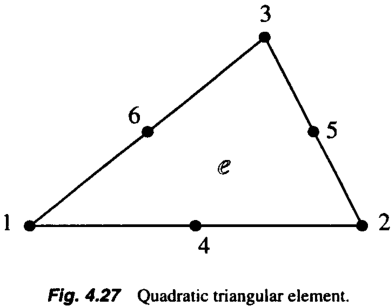
\includegraphics[scale=0.5]{inset/quadratic-triangular}

quadratic triangular element 的 elemental matrix 是 $6\times6$ 矩阵,它的元素是
\begin{align}
K_{ij} & =\iint_{\Omega^{e}}\left(\alpha_{x}\frac{\partial N_{i}^{e}}{\partial x}\frac{\partial N_{j}^{e}}{\partial x}+\alpha_{y}\frac{\partial N_{i}^{e}}{\partial y}\frac{\partial N_{j}^{e}}{\partial y}+\beta N_{i}^{e}N_{j}^{e}\right)\dd{x}\dd{y}\nonumber \\
 & i,j=1,2,3,\cdots6.\label{eq:4.151}
\end{align}
类似地,列 $\left\{ b^{e}\right\} $ 的元素为
\begin{equation}
b_{i}^{e}=\iint_{\Omega^{e}}fN_{i}^{e}\dd{x}\dd{y},\quad i,j=1,2,3,\cdots6.\label{eq:4.152}
\end{equation}


\subsection{4.7.1 Quadratic Triangular Elements}

page 83

\begin{equation}
L_{j}^{e}\left(x,y\right)=\frac{1}{2\Delta^{e}}\left(a_{j}^{e}+b_{j}^{e}x+c_{j}^{e}y\right),\quad j=1,2,3\label{eq:4.149}
\end{equation}
其中 $a_{j}^{e}$$b_{j}^{e}$$c_{j}^{e}$和 $\Delta^{e}$的定义和(4.24)中的相同。

\subsection{4.7.2 构建插值函数}

page 84

上述的方法可以用于构建任意阶单元的插值函数,然而有必要寻找一种简单的方法。下面的方法基于 Lagrangian interpolation
polynomials。再次观察(\ref{eq:4.149})中定义的 $L_{j}^{e}$。

\includegraphics[scale=0.5]{inset/FEMEM-4\lyxdot 28}

考虑三角单元中的一点$P$,由点$P$和节点$2$和$3$定义的三角形的面积为
\begin{align}
\Delta_{1} & =\frac{1}{2}\left|\begin{array}{ccc}
1 & x & y\\
1 & x_{2}^{e} & y_{2}^{e}\\
1 & x_{3}^{e} & y_{3}^{e}
\end{array}\right|\nonumber \\
 & =\frac{1}{2}\left[\left(x_{2}^{e}y_{3}^{e}-x_{3}^{e}y_{2}^{e}\right)+x\left(y_{2}^{e}-y_{3}^{e}\right)+y\left(x_{3}^{e}-x_{2}^{e}\right)\right].\label{eq:4.155}
\end{align}
使用前文(\ref{eq:4.24-1}) 定义的 $a_{j}^{e}$,$b_{j}^{e}$和$c_{j}^{e}$,$\Delta_{1}$可以写成
\begin{equation}
\Delta_{1}=\frac{1}{2}\left(a_{1}^{e}+b_{1}^{e}x+c_{1}^{e}y\right).\label{eq:4.156}
\end{equation}
与(\ref{eq:4.149})
\[
L_{j}^{e}\left(x,y\right)=\frac{1}{2\Delta^{e}}\left(a_{j}^{e}+b_{j}^{e}x+c_{j}^{e}y\right),\quad j=1,2,3
\]
比较,容易看出
\begin{equation}
L_{1}^{e}=\frac{\Delta_{1}}{\Delta^{e}}=\frac{1}{2\Delta^{e}}\left(a_{1}^{e}+b_{1}^{e}x+c_{1}^{e}y\right).\label{eq:4.157}
\end{equation}
类似地,我们发现
\begin{equation}
L_{2}^{e}=\frac{\Delta_{2}}{\Delta^{e}}=\frac{1}{2\Delta^{e}}\left(a_{2}^{e}+b_{2}^{e}x+c_{2}^{e}y\right).\label{eq:4.158}
\end{equation}
以及
\begin{equation}
L_{3}^{e}=\frac{\Delta_{3}}{\Delta^{e}}=\frac{1}{2\Delta^{e}}\left(a_{3}^{e}+b_{3}^{e}x+c_{3}^{e}y\right).\label{eq:4.159}
\end{equation}
其中$\Delta_{2}$标记由点$P$和节点$3$,节点$1$定义的三角形,$\Delta_{3}$标记由点$P$和节点$1,2$定义的三角形。由于点$P$的选取完全确定了$L_{1}^{e}$,$L_{2}^{e}$和$L_{3}^{e}$,所以也可以反过来,用后者定义一个唯一点$P$,由此也把
$\left(L_{1}^{e},L_{2}^{e},L_{3}^{e}\right)$ 称为面积坐标。在文献中,它们也被称为 \textbf{自然或单形坐标}(simplex
coordinates)。(\ref{eq:4.157})–(\ref{eq:4.159})可以紧凑地写成
\begin{equation}
\left\{ \begin{array}{c}
L_{1}^{e}\\
L_{2}^{e}\\
L_{3}^{e}
\end{array}\right\} =\frac{1}{2\Delta^{e}}\left[\begin{array}{ccc}
a_{1}^{e} & b_{1}^{e} & c_{1}^{e}\\
a_{2}^{e} & b_{2}^{e} & c_{2}^{e}\\
a_{3}^{e} & b_{3}^{e} & c_{3}^{e}
\end{array}\right]\left\{ \begin{array}{c}
1\\
x\\
y
\end{array}\right\} \label{eq:4.160}
\end{equation}
\textcolor{blue}{$L_{j}^{e}$正好是线性三角形单元的插值函数。}易得逆变换矩阵
\begin{equation}
\left\{ \begin{array}{c}
1\\
x\\
y
\end{array}\right\} =\left[\begin{array}{ccc}
1 & 1 & 1\\
x_{1}^{e} & x_{2}^{e} & x_{3}^{e}\\
y_{1}^{e} & y_{2}^{e} & y_{3}^{e}
\end{array}\right]\left\{ \begin{array}{c}
L_{1}^{e}\\
L_{2}^{e}\\
L_{3}^{e}
\end{array}\right\} .\label{eq:4.161}
\end{equation}

此坐标变换把 $\left(x,y\right)$ 平面上的任意形状三角形,变换到 $L_{i}$ 平面上的 等腰直角三角形。

\subsection{4.7.3 数值积分}

ref: The finite element method in electromagnetics; JianMing Jin;
4.7.3 page 148 (87)

此外, 可以借助数值积分方法。经常使用的数值积分方案是 Gauss quadrature,在 Sect 3.6 中讨论了一维积分的方法。对于在三角形单元上的积分,文献{[}9{]}中证明了
\begin{equation}
\iint_{\Omega^{e}}F\left(L_{1}^{e},L_{2}^{e},L_{3}^{e}\right)\dd{x}\dd{y}=\sum_{i=1}^{m}F\left(L_{1i}^{e},L_{2i}^{e},L_{3i}^{e}\right)W_{i}\Delta^{e}\label{eq:4.164}
\end{equation}
其中 $\left(L_{1i}^{e},L_{2i}^{e},L_{3i}^{e}\right)$ 表示采样点(sampling
points),$W_{i}$ 表示权重,在表 4.1中给出;$\Delta^{e}$表示$\left(x,y\right)$坐标空间中三角元的面积,来自于坐标变换的雅可比行列式。

记被积函数的 polynomial degree 为 $p$:
\begin{enumerate}
\item 若 $p\le1$,当 $m=1$ 即可积出精确值。
\item 若 $p\le2$,当 $m=3$ 即可积出精确值。
\item 若 $p\le3$,当 $m=4$ 即可积出精确值。
\item 若 $p\le4$,当 $m=7$ 即可积出精确值。
\end{enumerate}
$p$直到20,都可以应用 Gauss quadrature 规则。

\begin{table}[H]
\begin{tabular}{|c|c|c|c|c|c|c|c|}
\hline 
图 & $m$ & $p$ & $i$ & $L_{1i}^{e}$ & $L_{2i}^{e}$ & $L_{3i}^{e}$ & $W_{i}$\tabularnewline
\hline 
\hline 
\multirow{3}{*}{重心采点 $(1)$} & $1$ & $1$ & $1$ & $0.33333333$ & $0.33333333$ & $0.33333333$ & $1.00000000$\tabularnewline
\cline{2-8} \cline{3-8} \cline{4-8} \cline{5-8} \cline{6-8} \cline{7-8} \cline{8-8} 
 &  &  &  &  &  &  & \tabularnewline
\cline{2-8} \cline{3-8} \cline{4-8} \cline{5-8} \cline{6-8} \cline{7-8} \cline{8-8} 
 &  &  &  &  &  &  & \tabularnewline
\hline 
\multirow{3}{*}{边心采点 $(3)$} & $3$  & $2$ & $1$ & $0.500000000$ & $0.500000000$ & $0.00000000$ & $0.33333333$\tabularnewline
\cline{2-8} \cline{3-8} \cline{4-8} \cline{5-8} \cline{6-8} \cline{7-8} \cline{8-8} 
 &  &  & $2$ & $0.00000000$ & $0.500000000$ & $0.500000000$ & $0.33333333$\tabularnewline
\cline{2-8} \cline{3-8} \cline{4-8} \cline{5-8} \cline{6-8} \cline{7-8} \cline{8-8} 
 &  &  & $3$ & $0.500000000$ & $0.00000000$ & $0.500000000$ & $0.33333333$\tabularnewline
\hline 
\multirow{4}{*}{重心+内部 $(4)$} & $4$ & $3$ & $1$ & $0.33333333$ & $0.33333333$ & $0.33333333$ & $-0.56250000$\tabularnewline
\cline{2-8} \cline{3-8} \cline{4-8} \cline{5-8} \cline{6-8} \cline{7-8} \cline{8-8} 
 &  &  & $2$ & $0.73333333$ & $0.13333333$ & $0.13333333$ & $0.52083333$\tabularnewline
\cline{2-8} \cline{3-8} \cline{4-8} \cline{5-8} \cline{6-8} \cline{7-8} \cline{8-8} 
 &  &  & $3$ & $0.13333333$ & $0.73333333$ & $0.13333333$ & $0.52083333$\tabularnewline
\cline{2-8} \cline{3-8} \cline{4-8} \cline{5-8} \cline{6-8} \cline{7-8} \cline{8-8} 
 &  &  & $4$ & $0.13333333$ & $0.13333333$ & $0.73333333$ & $0.52083333$\tabularnewline
\hline 
\end{tabular}

\caption{三角形的 Gauss Quadrature 的采样点和权重}
\end{table}

\begin{rem}
令 $J$ 表示几何坐标对等参坐标的雅可比矩阵,$\det[J]$正比于几何区域的面积,例如对于三角形
\[
S=\frac{1}{2}\det[J]
\]
在计算程序中,这个几何常数被吸收进 权重因子 $W_{i}$ 中。因此程序中高斯积分法的形式为:
\[
\iint_{\Omega^{e}}F\left(L_{1}^{e},L_{2}^{e},L_{3}^{e}\right)\dd{x}\dd{y}=\sum_{i=1}^{m}F\left(L_{1i}^{e},L_{2i}^{e},L_{3i}^{e}\right)W_{i}^{\prime}\det[J]
\]
\end{rem}

\chapter{三维有限元分析,p99/96}

\label{chap:5}

所考虑的边值问题,可以用二阶微分方程表述
\begin{equation}
-\partial_{x}\left(\alpha_{x}\partial_{x}\phi\right)-\partial_{y}\left(\alpha_{y}\partial_{y}\phi\right)-\partial_{z}\left(\alpha_{z}\partial_{z}\phi\right)+\beta\phi=f,\quad\left(x,y,z\right)\in V\label{eq:5.1}
\end{equation}
并连同边值条件
\begin{equation}
\phi=p\quad\text{on}\quad S_{1}\label{eq:5.2}
\end{equation}
and 
\begin{equation}
\left(\alpha_{x}\partial_{x}\phi\hat{x}+\alpha_{y}\partial_{y}\phi\hat{y}+\alpha_{z}\partial_{z}\phi\hat{z}\right)\cdot\hat{n}+\gamma\phi=q\quad\text{on}\quad S_{2}\label{eq:5.3}
\end{equation}
其中 $S\left(=S_{1}+S_{2}\right)$ 标记闭合体积$V$的曲面,$\hat{n}$ 是指向外面的单位向量。

\section{边值问题}

\section{变分公式}

\section{有限元分析}

\subsection{区域离散化,Domain Discretization}

\begin{equation}
\phi^{e}\left(x,y,z\right)=\sum_{j=1}^{4}N_{j}^{e}\left(x,y,z\right)\phi_{j}^{e}\label{eq:5.10}
\end{equation}
\begin{align}
K_{ij}^{e} & =\iiint_{V}\left(\alpha_{x}\partial_{x}N_{i}^{e}\,\partial_{x}N_{j}^{e}+\alpha_{y}\partial_{y}N_{i}^{e}\,\partial_{y}N_{j}^{e}+\alpha_{z}\partial_{z}N_{i}^{e}\,\partial_{z}N_{j}^{e}\right)\dd{V}\label{eq:5.17}\\
b_{i}^{e} & =\iiint_{V}fN_{i}^{e}\dd{V}\label{eq:5.18}
\end{align}
显然 $[K^{e}]$ 是对称矩阵。

\subsection{Ritz 方法的 Formulation}

\subsection{Galerkin 方法的 Formulation}

(\ref{eq:5.1}) 对应的 residual error 是
\begin{align}
R_{i}^{e} & =\sum_{j=1}^{r}\phi_{j}^{e}\iiint_{V^{e}}\left(\alpha_{x}\partial_{x}N_{i}^{e}\,\partial_{x}N_{j}^{e}+\alpha_{y}\partial_{y}N_{i}^{e}\,\partial_{y}N_{j}^{e}+\alpha_{z}\partial_{z}N_{i}^{e}\,\partial_{z}N_{j}^{e}+\beta N_{i}^{e}N_{j}^{e}\right)\dd{V}\nonumber \\
 & -\iiint_{V^{e}}N_{i}^{e}f\dd{V}-\oint_{S^{e}}N_{i}^{e}\sbf D\cdot\hat{n}^{e}\dd{S}.\label{eq:5.42}
\end{align}
写成矩阵形式是
\begin{equation}
\left\{ R^{e}\right\} =\left[K^{e}\right]\left\{ \phi^{e}\right\} -\left\{ b^{e}\right\} -\left\{ g^{e}\right\} .\label{eq:5.43}
\end{equation}
$\left[K^{e}\right]$ 和 $\left\{ b^{e}\right\} $ 中的元素与(\ref{eq:5.17})
和 (\ref{eq:5.18}) 中的相同。

\noindent\fbox{\begin{minipage}[t]{1\columnwidth - 2\fboxsep - 2\fboxrule}%
\begin{align}
K_{ij}^{e} & =\iiint_{V}\left(\alpha_{x}\partial_{x}N_{i}^{e}\,\partial_{x}N_{j}^{e}+\alpha_{y}\partial_{y}N_{i}^{e}\,\partial_{y}N_{j}^{e}+\alpha_{z}\partial_{z}N_{i}^{e}\,\partial_{z}N_{j}^{e}\right)\dd{V}\label{eq:5.17-1}\\
b_{i}^{e} & =\iiint_{V}fN_{i}^{e}\dd{V}\label{eq:5.18-1}
\end{align}
%
\end{minipage}}

$\left\{ g^{e}\right\} $中的元素为
\begin{equation}
g_{i}^{e}=\oint_{S^{e}}N_{i}^{e}\sbf D\cdot\hat{n}^{e}\dd{S}\cdot\label{eq:5.44}
\end{equation}


\section{矩形块单元}

\section{静电问题的应用}

\section{静磁问题的应用}

\subsection{问题的描述}

\begin{equation}
\nabla\times(\frac{1}{\mu_{r}}\nabla\times\sbf A)=\mu_{0}\sbf J\label{eq:5.60}
\end{equation}


\paragraph{狄利克雷边界条件}

\begin{equation}
\hat{\sbf n}\times\sbf A=\sbf P\quad\text{在}S_{1}\text{上}\label{eq:5.61}
\end{equation}
如果在局部坐标系中为 $\sbf n=(0,0,1)$,则
\begin{equation}
{\color{blue}\hat{\sbf n}\times\sbf A=(-A_{y},A_{x})}=(P_{x},P_{y})\label{eq:5.61b}
\end{equation}
即约束$\sbf A$的切向分量 $\{A_{x},A_{y}\}$,因此将约束$\sbf A$在Edges上的环路积分 $\int\sbf A\cdot\dd{\sbf\ell}$。

\paragraph{适用于对称面的齐次诺伊曼条件}

\begin{equation}
\hat{\sbf n}\times(\nabla\times\sbf A)=0,\quad\text{在}S_{2}\text{上}\label{eq:5.62}
\end{equation}
同样在局部坐标系$\sbf n=(0,0,1)$中,
\[
\nabla\times\sbf A=(\partial_{y}A_{z}-\partial_{z}A_{y},\,{\color{blue}\partial_{z}A_{x}-\partial_{x}A_{z}},\,\partial_{x}A_{y}-\partial_{y}A_{x})
\]
则套用(\ref{eq:5.61b}),
\[
\hat{\sbf n}\times(\nabla\times\sbf A)=(-{\color{blue}\mathrm{curl}_{y}},\,\mathrm{curl}_{x})=(0,0)
\]
即约束$\sbf A$的旋度的切向分量。

\paragraph{介质分界面的连续性条件}

\begin{equation}
\hat{\sbf n}\times\sbf A^{+}=\hat{\sbf n}\times\sbf A^{-},\quad\text{在}S_{d}\text{上}\label{eq:5.63}
\end{equation}
\begin{equation}
\frac{1}{\mu_{r}^{+}}\hat{\sbf n}\times\nabla\times\sbf A^{+}=\frac{1}{\mu_{r}^{-}}\hat{\sbf n}\times\nabla\times\sbf A^{-},\quad\text{在}S_{d}\text{上}\label{eq:5.64}
\end{equation}
它们是连续性条件 $\hat{\sbf n}\cdot\sbf B^{+}=\hat{\sbf n}\cdot\sbf B^{-}$和
$\hat{\sbf n}\times\sbf H^{+}=\hat{\sbf n}\times\sbf H^{-}$的直接结果。

\subsection{变分公式}

\begin{equation}
F(\sbf A)=\frac{1}{2}\int_{V}\frac{1}{\mu_{r}}(\nabla\times\sbf A)\cdot(\nabla\times\sbf A)\dd{V}-\mu_{0}\int_{V}\sbf J\cdot\sbf A\dd{V}\label{eq:5.65}
\end{equation}

\begin{rem}
有矢量恒等式
\[
\nabla\cdot({\color{blue}\sbf a}\times\sbf b)=\sbf b\cdot\nabla\times\sbf a-\sbf a\cdot\nabla\times\sbf b
\]
代入$\sbf b={\color{red}\delta\sbf A}$,$\sbf a={\color{blue}\nabla\times\sbf A}$
得
\[
\nabla\cdot\left[({\color{blue}\nabla\times\sbf A})\times{\color{red}\delta\sbf A}\right]={\color{red}\delta\sbf A}\cdot\nabla\times({\color{blue}\nabla\times\sbf A})-({\color{blue}\nabla\times\sbf A})\cdot(\nabla\times{\color{red}\delta\sbf A})
\]
在考虑散度定理$\int_{v}\nabla\cdot\sbf f\dd{V}=\int_{S}\hat{\sbf n}\cdot\sbf f\dd{S}$
\begin{align*}
\nabla\cdot\left[({\color{blue}\nabla\times\sbf A})\times{\color{red}\delta\sbf A}\right] & \Rightarrow\sbf n\cdot\left[({\color{blue}\nabla\times\sbf A})\times{\color{red}\delta\sbf A}\right]\\
 & ={\color{red}\delta\sbf A}\cdot\left[\sbf n\times({\color{blue}\nabla\times\sbf A})\right]
\end{align*}
因此 \textbf{在积分号下} 有
\begin{align*}
\int_{V}({\color{blue}\nabla\times\sbf A})\cdot(\nabla\times{\color{red}\delta\sbf A})= & \int_{V}\left(\nabla\times{\color{blue}\nabla\times\sbf A}\right)\cdot{\color{red}\delta\sbf A}\\
 & -\int_{S_{2}}\left(\sbf n\times{\color{blue}\nabla\times\sbf A}\right)\cdot{\color{red}\delta\sbf A}
\end{align*}
\end{rem}
%
\begin{rem}
类似地,
\begin{align*}
\int_{V}({\color{blue}\nabla\times\sbf A})\cdot(\nabla\times{\color{red}\sbf A})= & \int_{V}\left(\nabla\times{\color{blue}\nabla\times\sbf A}\right)\cdot{\color{red}\sbf A}\\
 & -\int_{S_{2}}\left(\sbf n\times{\color{blue}\nabla\times\sbf A}\right)\cdot{\color{red}\sbf A}
\end{align*}
即 \textbf{curl 的模方}等于\textbf{二阶curl的投影}减去\textbf{curl切向分量的投影}。
\end{rem}
%
\begin{align*}
\delta F(\sbf A)= & \int_{V}\left[\nabla\times(\frac{1}{\mu_{r}}\nabla\times\sbf A)-\mu_{0}\sbf J\right]\cdot\delta\sbf A\dd{V}\\
 & -\int_{S_{d}}\left[\frac{1}{\mu_{r}^{+}}\left(\hat{\sbf n}\times\nabla\times\sbf A^{+}\right)-\frac{1}{\mu_{r}^{+}}\left(\hat{\sbf n}\times\nabla\times\sbf A^{-}\right)\right]\cdot\delta\sbf A\dd{S}\\
 & -\int_{S_{2}}\frac{1}{\mu_{r}}\left(\hat{\sbf n}\times\nabla\times\sbf A\right)\cdot\delta\sbf A\dd{S}
\end{align*}
其中$S_{2}$表示诺伊曼边界,$\hat{n}\times\delta\sbf A$在狄利克雷边界$S_{1}$上为零。$\delta F(\sbf A)=0$
意味着$\sbf A$必须满足 (\ref{eq:5.60}),(\ref{eq:5.62}),(\ref{eq:5.64})。
\begin{xca}
从下式

\[
R_{p\alpha}^{e}=\int_{V^{e}}N_{\alpha}^{e}\,\hat{\sbf p}\cdot\left[\nabla\times\left(\frac{1}{\mu_{r}}\nabla\times\sbf A\right)-\mu_{0}\sbf J\right]\dd{V},\quad p=x,y,z
\]
\end{xca}

\section{时谐场问题的应用p114/111}

\subsection{问题的描述}

\begin{equation}
\nabla\times\left(\frac{1}{\mu_{r}}\nabla\times\sbf E\right)-k_{0}^{2}\varepsilon_{r}\,\sbf E=-i\,k_{0}Z_{0}\sbf J\label{eq:5.101}
\end{equation}
\begin{equation}
\nabla\times\left(\frac{1}{\varepsilon_{r}}\nabla\times\sbf H\right)-k_{0}^{2}\mu_{r}\,\sbf H=\nabla\times\left(\frac{1}{\varepsilon_{r}}\sbf J\right)\label{eq:5.102}
\end{equation}
其中$Z_{0}=\sqrt{\mu_{0}/\varepsilon_{0}}$。

\paragraph{导电面上的边界条件}

\begin{equation}
\hat{\sbf n}\times\sbf E=0\label{eq:5.103}
\end{equation}
i.e.
\[
(-E_{y},E_{x})=(0,0)
\]
and
\begin{equation}
\hat{\sbf n}\times\nabla\times\sbf H=0\label{eq:5.104}
\end{equation}
\[
(-{\color{blue}\mathrm{curl}H_{y}},\,\mathrm{curl}H_{x})=(0,0)
\]

\begin{rem}
Note:
\begin{enumerate}
\item 有矢量恒等式
\begin{align*}
\varepsilon_{mni}{\color{blue}\partial_{n}}\,\varepsilon_{ijk}\partial_{j}H_{k} & =\left(\delta_{mj}\delta_{nk}-\delta_{nj}\delta_{mk}\right){\color{blue}\partial_{n}}\partial_{j}H_{k}\\
 & ={\color{blue}\partial_{k}}\partial_{m}H_{k}-{\color{blue}\partial_{n}}\partial_{n}\,H_{m}
\end{align*}
即
\[
\nabla\times(\nabla\times\sbf H)=\nabla(\nabla\cdot\sbf H)-\nabla^{2}\sbf H
\]
类似地有
\[
\sbf n\times(\nabla\times\sbf H)=(\nabla\sbf H)\cdot\sbf n-(\sbf n\cdot\nabla)\sbf H
\]
其中$\nabla\sbf H$表示并矢。如果$\sbf n$是常矢量(或者在局部)也可写成
\[
\sbf n\times(\nabla\times\sbf H)=\nabla(\sbf n\cdot\sbf H)-\sbf n\cdot(\nabla\sbf H)
\]
\item $\hat{\sbf n}\times\nabla\times\sbf H=0$ reads as,在边界上$\sbf H$的旋度的切向分量为零。如图选取合适的积分回路,令切向积分可以忽略,然后得到在边界面上$\sbf H$的法向分量处处相等。
\\
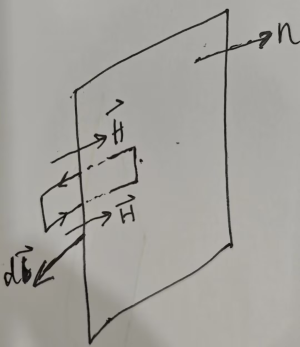
\includegraphics[scale=0.4]{inset/fig-boundary-condition-1}
\end{enumerate}
\end{rem}

\paragraph{导磁面上的对偶条件}

\begin{equation}
\hat{\sbf n}\times\nabla\times\sbf E=0\label{eq:5.105}
\end{equation}
\[
(-{\color{blue}\mathrm{curl}E_{y}},\,\mathrm{curl}E_{x})=(0,0)
\]
\begin{equation}
\hat{\sbf n}\times\sbf H=0\label{eq:5.106}
\end{equation}

\[
(-H_{y},H_{x})=(0,0)
\]


\paragraph{第三类边界条件}

\begin{align}
 & \frac{1}{\mu_{r}}\hat{\sbf n}\times\left(\nabla\times\sbf E\right)+\gamma_{e}\hat{\sbf n}\times\left(\hat{\sbf n}\times\sbf E\right)=\sbf U\label{eq:5.107}\\
 & \frac{1}{\varepsilon_{r}}\hat{\sbf n}\times\left(\nabla\times\sbf H\right)+\gamma_{h}\hat{\sbf n}\times\left(\hat{\sbf n}\times\sbf H\right)=\sbf V\label{eq:5.108}
\end{align}
$\sbf n=(0,0,1)$局部坐标下的分量形式
\[
\frac{1}{\mu_{r}}(-{\color{blue}\mathrm{curl}E_{y}},\,\mathrm{curl}E_{x})+\gamma_{e}\left(-E_{x},-E_{y}\right)=\left(U_{x},U_{y}\right)
\]
其中 $\gamma_{e}$和$\gamma_{h}$是已知参数,$\sbf U$和$\sbf V$是已知矢量。

两种不同媒质分界面上的连续性条件为
\begin{align}
 & \hat{\sbf n}\times\sbf E^{+}=\hat{\sbf n}\times\sbf E^{-}\label{eq:5.109}\\
 & \hat{\sbf n}\times\sbf H^{+}=\hat{\sbf n}\times\sbf H^{-}\label{eq:5.110}
\end{align}
也可将它们写成
\begin{align}
 & \frac{1}{\mu_{r}^{+}}\hat{\sbf n}\times(\nabla\times\sbf E^{+})=\frac{1}{\mu_{r}^{-}}\hat{\sbf n}\times(\nabla\times\sbf E^{-})\label{eq:5.111}\\
 & \frac{1}{\varepsilon_{r}^{+}}\hat{\sbf n}\times(\nabla\times\sbf H^{+})=\frac{1}{\varepsilon_{r}^{-}}\hat{\sbf n}\times(\nabla\times\sbf H^{-})\label{eq:5.112}
\end{align}

\begin{rem}
$\sbf n$的左叉乘相当于在$\sbf n$的法向上将矢量旋转$90\text{°}$。因此两次$\sbf n\times$算符相当于取切向投影的负号:
\[
\sbf n\times(\sbf n\times\sbf A)=-A_{t},
\]
\end{rem}

\subsection{变分公式}

\begin{align}
F(\sbf E)= & \frac{1}{2}\int_{V}\left[\frac{1}{\mu_{r}}\left(\nabla\times\sbf E\right)\cdot\left(\nabla\times\sbf E\right)-k_{0}^{2}\varepsilon_{r}\,\sbf E\cdot\sbf E\right]\dd{V}\nonumber \\
 & +\int_{S_{2}}\left[\frac{\gamma_{e}}{2}\left(\hat{\sbf n}\times\sbf E\right)\cdot\left(\hat{\sbf n}\times\sbf E\right)+\sbf E\cdot\sbf U\right]\dd{S}\nonumber \\
 & +i\,k_{0}Z_{0}\int_{V}\sbf E\cdot\sbf J\dd{V}\label{eq:5.113}
\end{align}
\begin{align}
F(\sbf H)= & \frac{1}{2}\int_{V}\left[\frac{1}{\varepsilon_{r}}\left(\nabla\times\sbf H\right)\cdot\left(\nabla\times\sbf H\right)-k_{0}^{2}\mu_{r}\,\sbf H\cdot\sbf H\right]\dd{V}\nonumber \\
 & +\int_{S_{2}}\left[\frac{\gamma_{h}}{2}\left(\hat{\sbf n}\times\sbf H\right)\cdot\left(\hat{\sbf n}\times\sbf H\right)+\sbf H\cdot\sbf V\right]\dd{S}\nonumber \\
 & -\int_{V}\sbf H\cdot\left(\nabla\times\frac{1}{\varepsilon_{r}}\sbf J\right)\dd{V}\label{eq:5.114}
\end{align}

类似于标量情形,上面给出的泛函对$\varepsilon_{r}$,$\mu_{r}$,$\gamma_{e}$和$\gamma_{h}$为实数或复数时均成立。如果这些参数是实数,那么,我们可以选用下列其他形式的泛函
\begin{align}
F(\sbf E)= & \frac{1}{2}\int_{V}\left[\frac{1}{\mu_{r}}\left(\nabla\times\sbf E\right)\cdot\left(\nabla\times\sbf E\right)^{*}-k_{0}^{2}\varepsilon_{r}\,\sbf E\cdot\sbf E^{*}\right]\dd{V}\nonumber \\
 & +\frac{1}{2}\int_{S_{2}}\left[\gamma_{e}\left(\hat{\sbf n}\times\sbf E\right)\cdot\left(\hat{\sbf n}\times\sbf E\right)^{*}+\sbf E^{*}\cdot\sbf U+\sbf E\cdot\sbf U^{*}\right]\dd{S}\nonumber \\
 & +i\,k_{0}Z_{0}\frac{1}{2}\int_{V}\left(\sbf E^{*}\cdot\sbf J-\sbf E\cdot\sbf J^{*}\right)\dd{V}\label{eq:5.115}
\end{align}
注意最后一项有负号,是因为前面的虚数$i$。
\begin{align}
F(\sbf H)= & \frac{1}{2}\int_{V}\left[\frac{1}{\varepsilon_{r}}\left(\nabla\times\sbf H\right)\cdot\left(\nabla\times\sbf H\right)^{*}-k_{0}^{2}\mu_{r}\,\sbf H\cdot\sbf H^{*}\right]\dd{V}\nonumber \\
 & +\frac{1}{2}\int_{S_{2}}\left[\gamma_{h}\left(\hat{\sbf n}\times\sbf H\right)\cdot\left(\hat{\sbf n}\times\sbf H\right)^{*}+\sbf H^{*}\cdot\sbf V+\sbf H\cdot\sbf V^{*}\right]\dd{S}\nonumber \\
 & -\frac{1}{2}\int_{V}\left[\sbf H^{*}\cdot\left(\nabla\times\frac{1}{\varepsilon_{r}}\sbf J\right)+\sbf H\cdot\left(\nabla\times\frac{1}{\varepsilon_{r}}\sbf J\right)^{*}\right]\dd{V}\label{eq:5.116}
\end{align}
这两个泛函均是实值的。因此它们的驻点对应于极大值或极小值;前面的两个泛函,由于它们是复数,因此不存在这样的极大值或极小值。

\subsection{边界条件和界面条件的处理}

狄利克雷边界条件,例如(\ref{eq:5.103})。
\[
\hat{\sbf n}\times\sbf E=0
\]
分量形式
\begin{equation}
n_{x}E_{y}-n_{y}E_{x}=0,\quad n_{y}E_{z}-n_{z}E_{y}=0,\quad n_{z}E_{x}-n_{x}E_{z}=0\label{eq:5.117}
\end{equation}
其中$\sbf n=n_{x}\hat{\sbf x}+n_{y}\hat{\sbf y}+n_{z}\hat{\sbf z}$。然后,选择一非零分量,例如$n_{z}$,来消除其他两个分量
\begin{equation}
\frac{E_{x}}{n_{x}}=\frac{E_{z}}{n_{z}},\quad\frac{E_{y}}{n_{y}}=\frac{E_{z}}{n_{z}},\label{eq:5.118}
\end{equation}
即可实现狄利克雷边界条件的强加。

当然,假如 $n_{x}$或$n_{y}$是非零的,也可以选择$n_{x}$或$n_{y}$来消除其它两个分量。

磁场在导电面上满足的边界条件(\ref{eq:5.104})等价于 $\hat{\sbf n}\cdot\sbf H=0$,即
\begin{equation}
n_{x}H_{x}+n_{y}H_{y}+n_{z}H_{z}=0\label{eq:5.119}
\end{equation}
\begin{equation}
H_{z}=-\frac{n_{x}}{n_{z}}H_{x}-\frac{n_{y}}{n_{z}}H_{y}\label{eq:5.120}
\end{equation}

我们需要显示强加连续性条件(\ref{eq:5.109})和(\ref{eq:5.110}),
\begin{align*}
 & \hat{\sbf n}\times\sbf E^{+}=\hat{\sbf n}\times\sbf E^{-}\\
 & \hat{\sbf n}\times\sbf H^{+}=\hat{\sbf n}\times\sbf H^{-}
\end{align*}
而将(\ref{eq:5.111})和(\ref{eq:5.112})当作自然条件来自动满足。只要给每个节点赋单一的值,即可实现连续性条件(\ref{eq:5.109})和(\ref{eq:5.110})的强加。不幸的是,在实现上述过程时,我们也强加了法向场连续性,这与下列实际边界条件矛盾,
\begin{align}
 & \hat{\sbf n}\cdot(\varepsilon_{r}^{+}\sbf E^{+})=\hat{\sbf n}\cdot(\varepsilon_{r}^{-}\sbf E^{-})\label{eq:5.121}\\
 & \hat{\sbf n}\cdot(\mu_{r}^{+}\sbf H^{+})=\hat{\sbf n}\cdot(\mu_{r}^{-}\sbf H^{-})\label{eq:5.122}
\end{align}
\textbf{基于这种推理,只要在界面附近将网格细分即可解决这种问题}。

\paragraph{强加边界条件}

\begin{equation}
\left\{ \begin{array}{c}
E_{x}^{+}\\
E_{y}^{+}\\
E_{z}^{+}
\end{array}\right\} =\left[\begin{array}{ccc}
n_{x}^{2}e+1 & n_{x}n_{y}e & n_{x}n_{z}e\\
n_{x}n_{y}e & n_{y}^{2}e+1 & n_{y}n_{z}e\\
n_{x}n_{z}e &  & n_{z}^{2}e+1
\end{array}\right]\left\{ \begin{array}{c}
E_{x}^{-}\\
E_{y}^{-}\\
E_{z}^{-}
\end{array}\right\} \label{eq:5.127}
\end{equation}
式中
\[
e=\frac{\varepsilon_{r}^{-}}{\varepsilon_{r}^{+}}-1
\]
只要用$\mu_{r}$代替$\varepsilon_{r}$,即可得到磁场$\sbf H$的类似表达式。

\paragraph{计算法向分量}

\begin{equation}
\sum_{s}\iint_{S^{s}}\hat{\sbf n^{s}}\cdot\left(\varepsilon_{r}^{+}N_{j}^{s}\,\sbf E_{i}^{+}\right)\dd{S}=\sum_{s}\iint_{S^{s}}\hat{\sbf n^{s}}\cdot\left(\varepsilon_{r}^{-}N_{j}^{s}\,\sbf E_{i}^{-}\right)\dd{S}\label{eq:5.128}
\end{equation}
$\sbf E_{i}^{+}$表示节点$i$上的电场;$S^{s}$表示第$s$个三角形的面,$\hat{\sbf n}$表示其法向,$N_{j}^{s}$表示第$s$个三角形内,局部节点编号$j$的插值函数。$i,j,s$
的关系为 $\mathrm{ns}(j,s)=i$(局部$\to$全局编号映射表)。既然$\hat{\sbf n^{s}}$在三角形平面上有唯一的定义,则它可容易地被计算出。显而易见,如果我们将节点$i$上的单位矢量$\hat{\sbf n_{i}}$定义为
\begin{equation}
\hat{\sbf n}_{i}=\frac{\sbf n}{\abs{\sbf n}},\quad\sbf n=\sum_{s}\iint_{S^{s}}\hat{\sbf n^{s}}N_{j}^{s}\dd{S}\label{eq:5.129}
\end{equation}
则(\ref{eq:5.128})可写成
\begin{equation}
\hat{\sbf n_{i}}\cdot\left(\varepsilon_{r}^{+}\,\sbf E_{r}^{+}\right)=\hat{\sbf n_{i}}\cdot\left(\varepsilon_{r}^{-}\,\sbf E_{r}^{-}\right)\label{eq:5.130}
\end{equation}
显然,单位矢量$\hat{\sbf n_{i}}$是局部加权平均,随着网格的细分,它收敛成实际光滑边界的唯一局部法向。因此可将$\hat{\sbf n_{i}}$当作节点$i$的平均法向,用它来实现(\ref{eq:5.128}),(\ref{eq:5.120})和\ref{eq:5.127}式给出的边界条件和界面条件。

\subsection{伪解问题}

$\nabla\times(\sbf E)/\mu_{r}$和$(\nabla\times\sbf H)/\varepsilon_{r}$必须是连续的。然而,我们在有限元求解过程中仅仅需要插值函数或展开函数连续,而对它们的导数则没有这种要求。这样得出的解叫作只在不太严格意义上满足控制微分方程的\textbf{弱解}。因为在弱解中
$\nabla\times(\sbf E)/\mu_{r}$和$(\nabla\times\sbf H)/\varepsilon_{r}$
不连续,所以我们不能取 (\ref{eq:5.101})和(\ref{eq:5.102})的散度来证明散度条件的满足。
\begin{align*}
 & \nabla\times\sbf E=-j\omega\sbf B\\
 & \nabla\times\sbf H=\sbf J+j\omega\sbf D
\end{align*}
更具体地说,如果对求电场感兴趣,可以先求磁场$\sbf H$,然后用麦克斯韦方程解出电场:
\begin{equation}
\sbf E=\frac{1}{j\omega\varepsilon}\left(\nabla\times\sbf H-\sbf J\right)\label{eq:5.131}
\end{equation}
这样即使$\sbf H$掺杂了伪解(非常可能)使用(\ref{eq:5.131})计算出的电场将不会包含伪解,满足散度条件。类似地,可以从电场得到磁场。
\begin{equation}
\sbf H=\frac{-1}{j\omega\mu}\nabla\times\sbf E\label{eq:5.132}
\end{equation}
上式可以保证磁场是无散的。不幸的是,因为导数运算,这样计算出的电场或磁场比直接用有限元求解的结果精度低。

\subsubsection{罚项}

\subsection{场的奇异性问题 p125/122}

\subsection{结论}

在这一节中,我们建立了三维时谐电磁场问题的有限元公式。用节点量插值的传统有限元时,我们遇到了三个主要困难。
\begin{itemize}
\item 媒质界面不连续
\item 非物理界或伪解
\item 不能模拟导体和材料的角、边缘和尖角处场的奇异性。
\end{itemize}
通过引入新型单元,不会出现困难。

\chapter{电磁学的变分原理 p128/125}

变分方法是通常用于建立有限元求解公式的两种方法之一。它的优点在于:有牢固的数理基础,其公式也有明确的物理解释。另一个优点在于:通过变分过程,我们能够清楚地说明必要边界条件和自然边界条件之间的区别,其他优点包括方便和公式优雅。

\section{标准变分原理\label{sec:6.1}}

page 128。标准变分原理复述如下:对下式微分方程定义的边值问题:
\begin{equation}
\mathcal{L}\Phi=f\label{eq:j6.1}
\end{equation}
如果算符是自伴的,即
\begin{equation}
\langle\Phi,\mathcal{L}\psi\rangle=\langle\mathcal{L}\Phi,\psi\rangle\label{eq:j6.2}
\end{equation}
 并且 $\mathcal{L}$ 是正定的,即
\begin{equation}
\langle\Phi,\mathcal{L}\Phi\rangle\begin{cases}
>0 & \Phi\neq0\\
=0 & \Phi=0
\end{cases}\label{eq:j6.3}
\end{equation}
那么,通过求下式泛函的极小值
\begin{equation}
F(\Phi)=\frac{1}{2}\langle\Phi,\mathcal{L}\Phi\rangle-\frac{1}{2}\langle\Phi,f\rangle-\frac{1}{2}\langle f,\Phi\rangle\label{eq:j6.4}
\end{equation}
即可求出(\ref{eq:j6.1})式的解。

在上面的几个式子中,$\psi$表示与$\Phi$满足相同边界条件的任意函数。\textbf{尖括号表示如下定义的内积}
\begin{equation}
\langle\Phi,\psi\rangle=\int_{\Omega}\Phi^{*}\psi\dd{\Omega}\label{eq:j6.5}
\end{equation}
式中,$\Omega$表示问题的区域,它可以是一维、二维和三维的;星号表示复共轭。为了证明这个变分原理,我们首先需要证明:
\begin{enumerate}
\item 微分方程(\ref{eq:j6.1})是当泛函$F$驻定时(即当$\delta F=0$时)的必然结果。
\item 然后,我们需要证明驻点是泛函$F$的极小值点。这等价于证明$\delta(\delta F)>0$。 
\end{enumerate}
\begin{align}
\delta F & =\frac{1}{2}\langle\delta\Phi,\mathcal{L}\Phi\rangle+\frac{1}{2}\langle\Phi,\mathcal{L}\delta\Phi\rangle-\frac{1}{2}\langle\delta\Phi,f\rangle-\frac{1}{2}\langle f,\delta\Phi\rangle\label{eq:j6.6}\\
 & =\frac{1}{2}\langle\delta\Phi,\mathcal{L}\Phi-f\rangle+\frac{1}{2}\langle\mathcal{L}\Phi-f,\delta\Phi\rangle\label{eq:j6.8}\\
 & =\ree\langle\delta\Phi,\mathcal{L}\Phi-f\rangle\label{eq:j6.9}
\end{align}
上式已使用了厄米性质 $\langle\mathcal{L}\delta\Phi,\Phi\rangle=\langle\delta\Phi,\mathcal{L}\Phi\rangle$以及内积的定义(\ref{eq:j6.5})。由于$\delta\Phi$是任意变分,所以从$\ree\langle\delta\Phi,\mathcal{L}\Phi-f\rangle=0$可以出的$\Phi$
必须满足(\ref{eq:j6.1})即 $\mathcal{L}\Phi=f$。
\begin{rem}
这里把复合微分算子$\mathcal{L}$看作类似系数矩阵的东西,把 $\Phi$ 看作自由度,因此不考虑$F(\Phi)$
对$\partial_{\mu}\phi$ 以及更高阶偏导的依赖,因为对 $\partial_{\mu}\phi$ 的依赖也已经考虑到算子$\mathcal{L}$中了,故写作$F(\phi)$。在这种框架下,欧拉–拉格朗日方程取简化形式
$\frac{\partial\mathcal{L}}{\partial\phi}=0$。

对于论点$2$,即$\delta(\delta F)>0$,再取 $\delta F$的第一变分,得到
\begin{equation}
\delta(\delta F)=\delta F(\Phi+\delta\Phi)-\delta F(\Phi)=\ree\langle\delta\Phi,\mathcal{L}\delta\Phi\rangle\label{eq:j6.11}
\end{equation}
既然$\mathcal{L}$是正定的。那么对于非零的$\delta\Phi$,可从(\ref{eq:j6.3})式得到$\delta(\delta F)>0$。因此,驻点确实是$F$的极小值点。
\end{rem}
%

\subsection{多场耦合}

考虑两个场 $\phi_{1},\phi_{2}$ 耦合的简单模型
\begin{align*}
\mathcal{F}(\phi_{i})= & \sum_{i=1,2}\frac{1}{2}\langle\phi_{i},\mathcal{L}_{i}\phi_{i}\rangle-\frac{1}{2}\langle\phi_{i},f_{i}\rangle-\frac{1}{2}\langle f_{i},\phi_{i}\rangle\\
 & +\frac{1}{2}\langle\phi_{1},\mathcal{L}_{12}\phi_{2}\rangle+\frac{1}{2}\langle\phi_{2},\mathcal{L}_{21}\phi_{1}\rangle
\end{align*}
\begin{align*}
\delta\mathcal{F}= & \sum_{i=1,2}\frac{1}{2}\langle\mathcal{L}_{i}\delta\phi_{i},\phi_{i}\rangle+\frac{1}{2}\langle\mathcal{L}_{i}\phi_{i},\delta\phi_{i}\rangle-\frac{1}{2}\langle\delta\phi_{i},f_{i}\rangle-\frac{1}{2}\langle f_{i},\delta\phi_{i}\rangle\\
 & +\frac{1}{2}{\color{blue}\langle\delta\phi_{1},\mathcal{L}_{12}\phi_{2}\rangle}+\frac{1}{2}{\color{brown}\langle\phi_{1},\mathcal{L}_{12}\delta\phi_{2}\rangle}+\frac{1}{2}{\color{blue}\langle\delta\phi_{2},\mathcal{L}_{21}\phi_{1}\rangle}+\frac{1}{2}{\color{brown}\langle\phi_{2},\mathcal{L}_{21}\delta\phi_{1}\rangle}\\
= & \frac{1}{2}\langle\delta\phi_{1},\mathcal{L}_{1}\phi_{1}-f_{1}+{\color{blue}\mathcal{L}_{12}\phi_{2}}\rangle+\frac{1}{2}\langle\mathcal{L}_{1}\phi_{1}-f_{1}+{\color{brown}\mathcal{L}_{21}\phi_{2}},\delta\phi_{1}\rangle\\
 & +\frac{1}{2}\langle\delta\phi_{2},\mathcal{L}_{2}\phi_{2}-f_{2}+{\color{blue}\mathcal{L}_{21}\phi_{1}}\rangle+\frac{1}{2}\langle\mathcal{L}_{2}\phi_{2}-f_{2}+{\color{brown}\mathcal{L}_{12}\phi_{1}},\delta\phi_{2}\rangle\\
= & \ree\langle\delta\phi_{1},\mathcal{L}_{1}\phi_{1}-f_{1}+{\color{blue}\mathcal{L}_{12}\phi_{2}}\rangle+\ree\langle\delta\phi_{2},\mathcal{L}_{2}\phi_{2}-f_{2}+{\color{blue}\mathcal{L}_{21}\phi_{1}}\rangle
\end{align*}
上面已经使用了厄米性质 $\langle\mathcal{L}\delta\phi_{i},\phi_{j}\rangle=\langle\delta\phi_{i},\mathcal{L}\phi_{j}\rangle$以及内积的定义$\langle\Phi,\psi\rangle=\int_{\Omega}\Phi\psi^{*}\dd{\Omega}$,以及
$\mathcal{L}_{12}^{*}=\mathcal{L}_{21}$。由于$\delta\phi_{i}$是任意变分,所以从$\ree\langle\cdots\rangle=0$
可以出的$\phi_{i}$ 必须满足的方程
\begin{align*}
 & \mathcal{L}_{1}\phi_{1}-f_{1}+{\color{blue}\mathcal{L}_{12}\phi_{2}}=0\\
 & \mathcal{L}_{2}\phi_{2}-f_{2}+{\color{blue}\mathcal{L}_{21}\phi_{1}}=0
\end{align*}

上面的式子可以简洁地写成矩阵的形式:
\[
F\left[\phi_{i}\right]=\frac{1}{2}\left[\begin{array}{cc}
\phi_{1} & \phi_{2}\end{array}\right]^{*}\left[\begin{array}{cc}
\mathcal{L}_{1} & \mathcal{L}_{12}\\
\mathcal{L}_{21} & \mathcal{L}_{2}
\end{array}\right]\left[\begin{array}{c}
\phi_{1}\\
\phi_{2}
\end{array}\right]-\frac{1}{2}\left[\begin{array}{cc}
\phi_{1} & \phi_{2}\end{array}\right]^{*}\left[\begin{array}{c}
f_{1}\\
f_{2}
\end{array}\right]-\frac{1}{2}\left[\begin{array}{cc}
f_{1} & f_{2}\end{array}\right]^{*}\left[\begin{array}{c}
\phi_{1}\\
\phi_{2}
\end{array}\right]
\]
\[
\left[\begin{array}{cc}
\mathcal{L}_{1} & \mathcal{L}_{12}\\
\mathcal{L}_{21} & \mathcal{L}_{2}
\end{array}\right]\left[\begin{array}{c}
\phi_{1}\\
\phi_{2}
\end{array}\right]=\left[\begin{array}{c}
f_{1}\\
f_{2}
\end{array}\right]
\]
或者
\[
F\left[\phi_{i}\right]=\frac{1}{2}\phi_{i}^{*}\mathcal{L}_{ij}\phi_{j}-\frac{1}{2}\phi_{i}^{*}f_{i}-\frac{1}{2}f_{i}^{*}\phi_{i}
\]
对应的方程为
\[
\mathcal{L}_{ij}\phi_{j}=f_{i}
\]
其中要求$\mathcal{L}$ 是厄米矩阵,$\mathcal{L}_{ji}^{*}=\mathcal{L}_{ij}$:对于对角元素,相当于要求它作用在$\phi_{i}$上是厄米的;对于非对角元素,相当于要求它对$\phi_{i}$内积是对称的。

\subsubsection{标准变分原理的例子}
\begin{example}
泊松方程
\begin{equation}
-\nabla\cdot(\varepsilon\nabla\Phi)=\rho\label{eq:j6.12}
\end{equation}
显然这个方程的算符为
\begin{equation}
\mathcal{L}=-\nabla\cdot(\varepsilon\nabla)\label{eq:j6.13}
\end{equation}

首先来验证$\mathcal{L}$满足(\ref{eq:j6.2}),即厄米条件。根据内积的定义,$\mathcal{L}$的作用是:
\begin{equation}
\langle\psi,\mathcal{L}\Phi\rangle=\int_{V}\psi^{*}[-\nabla\cdot(\varepsilon\nabla\Phi)]\dd{V}\label{eq:j6.14}
\end{equation}
使用第一标量格林定理(\ref{eq:jA.20})
\[
\int_{V}\left[a\nabla\cdot{\color{blue}(u\nabla b)}+u(\nabla a)\cdot(\nabla b)\right]\dd{V}=\oint_{S}a{\color{blue}u\frac{\partial b}{\partial n}}\dd{S}
\]
得到
\begin{equation}
\langle\psi,\mathcal{L}\Phi\rangle=\int_{V}\Phi[-\nabla\cdot(\varepsilon\nabla\psi^{*})]\dd{V}-\oint_{S}\varepsilon\left(\psi^{*}\frac{\partial\Phi}{\partial n}-\Phi\frac{\partial\psi^{*}}{\partial n}\right)\dd{S}\label{eq:j6.15}
\end{equation}
其中$\hat{\sbf n}$是$S$的外法向单位矢量。如果$\varepsilon$是实数或实函数,则上式右边第一项可写成$\langle\mathcal{L}\psi,\Phi\rangle$。第二项是面积分,如果$\Phi$和$\psi$均满足齐次狄利克雷边界条件(满足其一即可)
\begin{equation}
\Phi=0,\quad\text{在}S_{1}\text{上}\label{eq:j6.16}
\end{equation}
以及第三类齐次边界条件
\begin{equation}
\varepsilon\frac{\partial\Phi}{\partial n}+\gamma\Phi=0,\quad\text{在}S_{2}\text{上}\label{eq:j6.17}
\end{equation}
那么,(\ref{eq:j6.15})式右边第二项为零。上式中的$\varepsilon$和$\gamma$是实数,而$S_{1}+S_{2}=S$。在条件(\ref{eq:j6.16})和(\ref{eq:j6.17})式下,
(\ref{eq:j6.15})变成
\begin{equation}
\langle\psi,\mathcal{L}\Phi\rangle=\langle\mathcal{L}\psi,\Phi\rangle\label{eq:j6.18}
\end{equation}
即算符$\mathcal{L}$是自伴的条件为:
\end{example}
\begin{enumerate}
\item $\varepsilon$ 和 $\gamma$是实数;
\item 边界条件是齐次的。
\end{enumerate}
在这些条件下,将(\ref{eq:j6.13})式代入(\ref{eq:j6.14})中,即可建立泛函$F$如下:
\begin{equation}
F(\Phi)=\frac{1}{2}\int_{V}\Phi^{*}[-\nabla\cdot(\varepsilon\nabla\Phi)]\dd{V}-\frac{1}{2}\int_{V}\Phi\rho^{*}\dd{V}-\frac{1}{2}\int_{V}\rho\Phi^{*}\dd{V}\label{eq:j6.19}
\end{equation}
应用第一标量格林定理
\[
\int_{V}\left[a\nabla\cdot{\color{blue}(u\nabla b)}+u(\nabla a)\cdot(\nabla b)\right]\dd{V}=\oint_{S}a{\color{blue}u\frac{\partial b}{\partial n}}\dd{S}
\]
(\ref{eq:j6.19})式以及边界条件(\ref{eq:j6.16})和(\ref{eq:j6.17})式,上式可写成
\begin{equation}
F(\Phi)=\frac{1}{2}\int_{V}\varepsilon\abs{\nabla\Phi}^{2}\dd{V}+\frac{1}{2}\int_{S_{2}}\gamma\abs{\Phi}^{2}\dd{S}-\frac{1}{2}\int_{V}(\Phi\rho^{*}+\rho\Phi^{*})\dd{V}\label{eq:j6.20}
\end{equation}

\begin{example}
考虑下式简化情形
\begin{equation}
\langle\Phi,\mathcal{L}\Phi\rangle=\int_{V}\Phi^{*}[-\nabla\cdot(\varepsilon\nabla\Phi)]\dd{V}\label{eq:j6.21}
\end{equation}
应用第一标量格林定理,上式变成
\begin{equation}
\langle\Phi,\mathcal{L}\Phi\rangle=\int_{V}\varepsilon\nabla\Phi\cdot\nabla\Phi^{*}\dd{V}-\oint_{S}\varepsilon\Phi*\frac{\partial\Phi}{\partial n}\dd{S}\label{eq:j6.22}
\end{equation}
由于边界条件(\ref{eq:j6.16})和(\ref{eq:j6.17})式,(\ref{eq:j6.22})式变成
\begin{equation}
\langle\Phi,\mathcal{L}\Phi\rangle=\int_{V}\varepsilon\abs{\nabla\Phi}^{2}\dd{V}+\int_{S_{2}}\gamma\abs{\Phi}^{2}\dd{S}\label{eq:6.23}
\end{equation}
假设$\varepsilon$和$\gamma$非负,且它们不同时为零,显然当$\Phi\neq0$时,$\langle\Phi,\mathcal{L}\Phi\rangle>0$;当$\Phi=0$时,$\langle\mathcal{L}\Phi,\Phi\rangle=0$。因此,如果$\varepsilon$和$\gamma$是正数(非零),那么算符$\mathcal{L}$是正定的。在这个条件下,(\ref{eq:j6.12})式的解对应于(\ref{eq:j6.20})式中给出泛函的极小值。
\end{example}
%
\begin{example}
上面的过程也适用于矢量问题。在这种情形下,内积定义为
\begin{equation}
\langle\sbf a,\sbf b\rangle=\int_{V}\sbf a^{*}\cdot\sbf b\dd{V}\label{eq:j6.24}
\end{equation}
为了说明标准变分原理对矢量问题的应用及其限制,让我们考虑矢量波动方程
\begin{equation}
\nabla\times(\frac{1}{\mu_{r}}\nabla\times\sbf E)-k_{0}^{2}\sbf\varepsilon_{r}\sbf E=-jk_{0}Z_{0}\sbf J\label{eq:j6.25}
\end{equation}
其中$j$表示虚数单位。对于这种情形,算符$\mathcal{L}$可以写成
\begin{equation}
\mathcal{L}(\sbf f)=\nabla\times(\frac{1}{\mu_{r}}\nabla\times\sbf f)-k_{0}^{2}\sbf\varepsilon_{r}\sbf f\label{eq:j6.26}
\end{equation}
\end{example}

\section{修正变分原理}

从上节中给出的几个例子可以看到,为了应用标准变分原理,微分方程的算符必须是厄米的。
\begin{enumerate}
\item 对一个厄米算符,算符本身以及边界算符必须是实数或实函数。
\item 另外边界条件必须是齐次的。
\end{enumerate}
然而,在许多电磁学问题中,算符通常是复数或复函数,且边界条件也常常是非齐次的。因此去掉这两个条件十分重要,否则它们将严重限制变分方法的应用。我们在此只考虑第二个条件,将变分原理修正为能处理非齐次边界条件的变分方法。

考虑(\ref{eq:j6.1})定义的边值问题以及一组非齐次边界条件。
\begin{align*}
 & \mathcal{L}\Phi=f\\
 & \Phi=p,\quad\text{on}\quad S_{1}\\
 & \varepsilon\frac{\partial\Phi}{\partial n}+\gamma\Phi=q,\quad\text{on}\quad S_{2}
\end{align*}
式中$f$,$p$和$q$是已知参数。由前面的例子可见,这个问题是非厄米的,然而只要引进新的未知函数$\Phi'=\Phi-u$,非厄米问题即可转化成厄米问题。这里的$u$是满足给定非齐次边界条件的任意函数。结果新的函数$\Phi'$满足其次边界条件,因而问题可以变成厄米的。因此可以用标准变分原理来建立问题的泛函。将$\Phi=\Phi'+u$代入(\ref{eq:j6.1}),$\Phi'$的微分方程可以写成
\begin{equation}
\mathcal{L}\Phi'=f'\label{eq:j6.37}
\end{equation}
式中$f'=f-\mathcal{L}u$,因此(\ref{eq:j6.37})的泛函为
\begin{equation}
F(\Phi')=\frac{1}{2}\langle\Phi',\mathcal{L}\Phi'\rangle-\frac{1}{2}\langle\Phi',f'\rangle-\frac{1}{2}\langle f',\Phi'\rangle\label{eq:j6.38}
\end{equation}
即
\begin{align}
F(\Phi) & =\frac{1}{2}\langle(\Phi-u),\mathcal{L}(\Phi-u)\rangle-\frac{1}{2}\langle(\Phi-u),(f-\mathcal{L}u)\rangle\nonumber \\
 & \quad-\frac{1}{2}\langle(f-\mathcal{L}u),(\Phi-u)\rangle\label{eq:j6.39}
\end{align}
既然只对未知函数$\Phi$取变分,那么我们可以丢掉不含$\Phi$的项。因此泛函可写成
\begin{equation}
F(\Phi)=\frac{1}{2}\langle\Phi,\mathcal{L}\Phi\rangle-\frac{1}{2}\langle u,\mathcal{L}\Phi\rangle+\frac{1}{2}\langle\mathcal{L}u,\Phi\rangle-\frac{1}{2}\langle\Phi,f\rangle-\frac{1}{2}\langle f,\Phi\rangle\label{eq:j6.40}
\end{equation}
在这里并没有将 $-\frac{1}{2}\langle u,\mathcal{L}\Phi\rangle+\frac{1}{2}\langle\mathcal{L}u,\Phi\rangle$消去,因为在所考虑的非齐次边界条件下,不能武断的认为
$\mathcal{L}$ 是厄米的。

\subsection{边界条件的影响\label{subsec:bnd}}

\begin{align}
\delta F(\phi)= & \frac{1}{2}\left[{\color{blue}\langle\delta\Phi,\mathcal{L}\Phi\rangle}{\color{brown}+\langle\Phi,\mathcal{L}\delta\Phi\rangle-\langle u,\mathcal{L}\delta\Phi\rangle}{\color{red}+\langle\mathcal{L}u,\delta\Phi\rangle}{\color{blue}-\langle\delta\Phi,f\rangle}{\color{red}-\langle f,\delta\Phi\rangle}\right]\nonumber \\
 & =\frac{1}{2}\left[{\color{blue}\langle\delta\Phi,\mathcal{L}\Phi-f\rangle}{\color{brown}+\langle\Phi-u,\mathcal{L}\delta\Phi\rangle}{\color{red}+\langle\mathcal{L}u-f,\delta\Phi\rangle}\right]\label{eq:ym3}
\end{align}
由第二标量格林定理(\ref{eq:jA.20})
\[
\int_{V}\Phi^{*}\left[-\nabla\cdot(\varepsilon\nabla\Phi)\right]\dd{V}-\int_{V}\Phi\left[-\nabla\cdot(\varepsilon\nabla\Phi^{*})\right]\dd{V}=-\oint_{S}\varepsilon(\Phi^{*}\frac{\partial\Phi}{\partial n}-\Phi\frac{\partial\Phi^{*}}{\partial n})\dd{S}
\]
此表达式即$\langle\Phi,\mathcal{L}\Phi\rangle-\langle\mathcal{L}\Phi,\Phi\rangle$的余项。在边界$S_{1}$和$S_{2}$上分别讨论:
\begin{enumerate}
\item 在 $S_{1}$上,$\Phi=p$,则
\[
\Phi^{*}\frac{\partial\Phi}{\partial n}-\Phi\frac{\partial\Phi^{*}}{\partial n}=p^{*}\frac{\partial p}{\partial n}-p\frac{\partial p{}^{*}}{\partial n}
\]
若$p$是实数,显然有$\langle\Phi,\mathcal{L}\Phi\rangle=\langle\mathcal{L}\Phi,\Phi\rangle$。
\item 在$S_{2}$上,$\varepsilon\frac{\partial\Phi}{\partial n}=q-\gamma\Phi$,则
\begin{align*}
\Phi^{*}\frac{\partial\Phi}{\partial n}-\Phi\frac{\partial\Phi^{*}}{\partial n} & =\Phi^{*}(q-\gamma\Phi)-\Phi(q^{*}-\gamma\Phi^{*})\\
 & =\Phi^{*}q-\Phi q^{*}
\end{align*}
如果$\Phi$,$q$是实数,则也有$\langle\Phi,\mathcal{L}\Phi\rangle=\langle\mathcal{L}\Phi,\Phi\rangle$。
\item 前面假设了$u$和$\Phi$满足相同的边界条件,对于$\langle\Phi,\mathcal{L}u\rangle-\langle\mathcal{L}\Phi,u\rangle$的讨论是类似的,结果为
\[
\Phi^{*}(q-\gamma u)-u(q^{*}-\gamma\Phi^{*})
\]
\begin{align*}
 & \Phi^{*}\frac{\partial u}{\partial n}-u\frac{\partial\Phi^{*}}{\partial n}=p^{*}\frac{\partial p}{\partial n}-p\frac{\partial p{}^{*}}{\partial n},\quad\text{on}\;S_{1}\\
 & \Phi^{*}\frac{\partial u}{\partial n}-u\frac{\partial\Phi^{*}}{\partial n}=\Phi^{*}q-q^{*}u,\quad\text{on}\;S_{2}
\end{align*}
可以看出,在$S_{1}$上如果$p$是函数,则${\color{brown}\langle u,\mathcal{L}\delta\Phi\rangle=\langle\mathcal{L}u,\delta\Phi\rangle}$;在$S_{2}$上,即使$q$,$\Phi$,$u$都是实函数,$\Phi^{*}q-q^{*}u$
也未必为零,因而未必有${\color{brown}\langle u,\mathcal{L}\delta\Phi\rangle=\langle\mathcal{L}u,\delta\Phi\rangle}$。因此,在$S_{1}$上(\ref{eq:ym3})也许能获得简化
\begin{align*}
\delta F(\phi)= & \frac{1}{2}\left[{\color{blue}\langle\delta\Phi,\mathcal{L}\Phi-f\rangle}{\color{brown}+\langle\Phi-u,\mathcal{L}\delta\Phi\rangle}{\color{red}+\langle\mathcal{L}u-f,\delta\Phi\rangle}\right]\\
= & \frac{1}{2}\left[{\color{blue}\langle\delta\Phi,\mathcal{L}\Phi-f\rangle}{\color{brown}+\langle\mathcal{L}\Phi-\mathcal{L}u}{\color{red}+\mathcal{L}u-f},\delta\Phi\rangle\right]\\
= & \ree\langle\delta\Phi,\mathcal{L}\Phi-f\rangle
\end{align*}
但在$S_{2}$上却未必有$\delta F(\phi)=\ree\langle\delta\Phi,\mathcal{L}\Phi-f\rangle$。
\end{enumerate}
总结,$S_{1}$上的实函数第一类边界条件不会影响微分方程的成立,也就不影响有限元方程的建立;而$S_{2}$上的实函数第二类边界条件会有
non–trivial 的影响,会影响到边界$S_{2}$上方程的形式。

\subsection{应用举例}

在下面的例子中将会看出,上式右边的第二项和第三项通常可转化成边界积分或边界项,其中$u$在应用边界条件后消失。我们称上面描述的结果为
\textbf{修正变分原理},在此重述如下:给定边值问题(\ref{eq:j6.1})式,如果算符$\mathcal{L}$在齐次边界条件下是厄米的,那么其解可通过求泛函(\ref{eq:j6.40})式的驻点而得到,其中$u$是满足给定非齐次边界条件的任意函数。

现在,让我们用上节中的例子来说明修正变分原理的应用。考虑泊松方程(\ref{eq:j6.12})式所定义的问题以及下列边界条件:
\begin{align}
 & -\nabla\cdot(\varepsilon\nabla\Phi)=\rho\nonumber \\
 & \Phi=p,\quad\text{on}\quad S_{1}\label{eq:j6.41}\\
 & \varepsilon\frac{\partial\Phi}{\partial n}+\gamma\Phi=q,\quad\text{on}\quad S_{2}\label{eq:j6.42}
\end{align}
式中$p$和$q$是已知参数。正如在上节中所证明的那样,只要$\varepsilon$和$\gamma$是实数或实函数,算符$\mathcal{L}$在齐次边界条件下就是厄米的。因此将$\mathcal{L}=-\nabla\cdot(\varepsilon\nabla\cdots)$
和$f=\rho$ 代入(\ref{eq:j6.40})式,即可得到该问题的泛函$F(\Phi)$为
\begin{align}
F(\Phi)= & \frac{1}{2}\int_{V}\Phi^{*}\left[-\nabla\cdot(\varepsilon\nabla\Phi)\right]\dd{V}+\frac{1}{2}\int_{V}\left\{ u^{*}\left[\nabla\cdot(\varepsilon\nabla\Phi)\right]-\left[\nabla\cdot(\varepsilon\nabla u)\right]^{*}\Phi\right\} \dd{V}\nonumber \\
 & -\frac{1}{2}\int_{V}\left(\Phi^{*}\rho+\rho^{*}\Phi\right)\dd{V}\label{eq:j6.43}
\end{align}
式中$u$是满足(\ref{eq:j6.41})和(\ref{eq:j6.42})式的任意函数。应用第二标量格林定理(\ref{eq:jA.20})式
\[
\int_{V}\left[a\nabla\cdot{\color{blue}(u\nabla b)}-b\nabla\cdot{\color{brown}(u\nabla a)}\right]\dd{V}=\oint_{S}u({\color{blue}a\frac{\partial b}{\partial n}}{\color{brown}-b\frac{\partial a}{\partial n}})\dd{S}
\]
得到
\begin{align}
F(\Phi)= & \frac{1}{2}\int_{V}\Phi^{*}\left[-\nabla\cdot(\varepsilon\nabla\Phi)\right]\dd{V}-\frac{1}{2}\int_{V}\left(\Phi^{*}\rho+\rho^{*}\Phi\right)\dd{V}\nonumber \\
 & +\frac{1}{2}{\color{blue}\oint_{S}}\varepsilon\left(u^{*}\frac{\partial\Phi}{\partial n}-\Phi\frac{\partial u^{*}}{\partial n}\right)\dd{S}\label{eq:j6.44}
\end{align}
因为$\Phi$和$u$均满足边界条件(\ref{eq:j6.41})和(\ref{eq:j6.42})式,将它们应用于上式得到
\begin{align}
F(\Phi)= & \frac{1}{2}\int_{V}\Phi^{*}\left[-\nabla\cdot(\varepsilon\nabla\Phi)\right]\dd{V}-\frac{1}{2}\int_{V}\left(\Phi^{*}\rho+\rho^{*}\Phi\right)\dd{V}\nonumber \\
 & +\frac{1}{2}{\color{blue}\int_{S_{1}}}\varepsilon\left(p^{*}\frac{\partial\Phi}{\partial n}-p\frac{\partial u^{*}}{\partial n}\right)\dd{S}+\frac{1}{2}{\color{blue}\int_{S_{2}}}\left(qu^{*}-q^{*}\Phi\right)\dd{S}\label{eq:j6.45}
\end{align}
丢掉不包含$\Phi$的项,上式可写成
\begin{align}
F(\Phi)= & \frac{1}{2}\int_{V}\Phi^{*}\left[-\nabla\cdot(\varepsilon\nabla\Phi)\right]\dd{V}-\frac{1}{2}\int_{V}\left(\Phi^{*}\rho+\rho^{*}\Phi\right)\dd{V}\nonumber \\
 & +\frac{1}{2}{\color{blue}\int_{S_{1}}}\varepsilon p^{*}\frac{\partial\Phi}{\partial n}\dd{S}-\frac{1}{2}{\color{blue}\int_{S_{2}}}q^{*}\Phi\dd{S}\label{eq:j6.46}
\end{align}
应用(\ref{eq:jA.19})
\[
\int_{V}\left[a\nabla\cdot{\color{blue}(u\nabla b)}+u(\nabla a)\cdot(\nabla b)\right]\dd{V}=\oint_{S}a{\color{blue}u\frac{\partial b}{\partial n}}\dd{S},
\]
以及(\ref{eq:j6.41})、(\ref{eq:j6.42})的边界条件,代入中间等式
\begin{align*}
\int_{V}\Phi^{*}\left[-\nabla\cdot(\varepsilon\nabla\Phi)\right]\dd{V} & =\int_{V}\varepsilon\abs{\nabla\Phi}^{2}\dd{V}-\oint_{S_{1}+S_{2}}{\color{brown}\varepsilon\Phi^{*}\frac{\partial\Phi}{\partial n}}\dd{S}\\
\gamma\abs{\Phi}^{2}-q\Phi^{*} & =-{\color{brown}\varepsilon\Phi^{*}\frac{\partial\Phi}{\partial n}},\quad\text{on}\quad S_{2}
\end{align*}
边界项的变形为:
\begin{align*}
 & \frac{1}{2}\left[{\color{blue}\int_{S_{1}}}\varepsilon p^{*}\frac{\partial\Phi}{\partial n}\dd{S}-{\color{blue}\int_{S_{2}}}q^{*}\Phi\dd{S}\right]-\oint_{S_{1}+S_{2}}\cdots\dd{S}\\
\Rightarrow & \frac{1}{2}\left[{\color{blue}\int_{S_{1}}}\varepsilon(p^{*}-\Phi^{*})\frac{\partial\Phi}{\partial n}\dd{S}-{\color{blue}\int_{S_{2}}}q^{*}\Phi+\varepsilon\Phi^{*}\frac{\partial\Phi}{\partial n}\dd{S}\right]
\end{align*}
上式可写成对称形式
\begin{align}
\mathcal{F}(\Phi)= & \frac{1}{2}\int_{V}\varepsilon\abs{\nabla\Phi}^{2}\dd{V}-\frac{1}{2}\int_{V}\left(\Phi^{*}\rho+\rho^{*}\Phi\right)\dd{V}\nonumber \\
 & +\frac{1}{2}\int_{S_{2}}\left(\gamma\abs{\Phi}^{2}-q\Phi^{*}-q^{*}\Phi\right)\dd{S}\label{eq:j6.47}
\end{align}
其中$S_{1}$上的积分已经被消除。
\begin{rem}
当考虑的问题在实数域,即$\Phi,\rho,q,\gamma,\varepsilon$均为实函数,
\begin{align}
\mathcal{F}(\Phi)= & \frac{1}{2}\int_{V}\varepsilon(\nabla\Phi)\cdot\varepsilon(\nabla\Phi)\dd{V}-\int_{V}\Phi\rho\dd{V}\nonumber \\
 & +\int_{S_{2}}\left(\frac{1}{2}\gamma\Phi^{2}-q\Phi\right)\dd{S}\label{eq:j6.47c}
\end{align}
使用(\ref{eq:jA.19})将给出:
\begin{align}
\mathcal{F}(\Phi)= & \frac{1}{2}\int_{V}\Phi[-\nabla\cdot(\varepsilon\nabla\Phi)]\dd{V}-\int_{V}\Phi\rho\dd{V}\nonumber \\
 & +\int_{S_{2}}\left(\frac{\varepsilon}{2}\Phi\frac{\partial}{\partial n}\Phi+\frac{1}{2}\gamma\Phi^{2}-q\Phi\right)\dd{S}\label{eq:j6.47b}
\end{align}
其中$\frac{\partial}{\partial n}$理解为厄米算符,$\Phi\frac{\partial}{\partial n}\Phi$理解为二次型。这里再次列出对应的方程和边界条件:
\begin{align*}
 & -\nabla\cdot(\varepsilon\nabla\Phi)=\rho\\
 & \Phi=p,\quad\text{on}\quad S_{1}\\
 & \varepsilon\frac{\partial\Phi}{\partial n}+\gamma\Phi=q,\quad\text{on}\quad S_{2}
\end{align*}
\end{rem}

\subsection{多场耦合}

单场$\phi$的作用量$\mathcal{F}(\phi)$写作
\begin{align*}
\mathcal{F}(\phi)= & \frac{1}{2}\langle\phi',\mathcal{L}\phi'\rangle-\frac{1}{2}\langle\phi',f'\rangle-\frac{1}{2}\langle f',\phi'\rangle\\
= & \frac{1}{2}\langle\phi,\mathcal{L}\phi\rangle-\frac{1}{2}\langle u,\mathcal{L}\phi\rangle+\frac{1}{2}\langle\mathcal{L}u,\phi\rangle-\frac{1}{2}\langle\phi,f\rangle-\frac{1}{2}\langle f,\phi\rangle
\end{align*}
其中$\phi'=\phi-u$,$f'=f-\mathcal{L}u$,$u$是引入的任意函数,$u$和$\phi$均满足非齐次边界条件:
\begin{align*}
 & \Phi=p,\quad\text{on}\quad S_{1}\\
 & \varepsilon\frac{\partial\Phi}{\partial n}+\gamma\Phi=q,\quad\text{on}\quad S_{2}
\end{align*}

类似标准变分原理,将多场耦合的$\mathcal{F}(\phi)$用指标表示为

\begin{align*}
F\left[\phi_{i}\right] & =\frac{1}{2}\left(\phi_{i}-u_{i}\right)^{*}\mathcal{L}_{ij}\left(\phi_{j}-u_{j}\right)-\frac{1}{2}\left(\phi_{i}-u_{i}\right)^{*}\left(f_{i}-\mathcal{L}_{ij}u_{j}\right)-\frac{1}{2}\left(f_{i}-\mathcal{L}_{ij}u_{j}\right)^{*}\left(\phi_{i}-u_{i}\right)\\
 & =\frac{1}{2}\left[\phi_{i}^{*}\mathcal{L}_{ij}\phi_{j}{\color{blue}-u_{i}^{*}\mathcal{L}_{ij}\phi_{j}+\phi_{j}\mathcal{L}_{ji}^{*}u_{i}^{*}}-\phi_{i}^{*}f_{i}-f_{i}^{*}\phi_{i}\right]
\end{align*}
如同(\ref{subsec:bnd})那里所讨论的,由于考虑的非齐次边界条件,$u_{i}^{*}\mathcal{L}_{ij}\phi_{j}$
未必等于$\phi_{j}\mathcal{L}_{ji}^{*}u_{i}^{*}$,也就是 $\mathcal{L}_{ji}^{*}$
在此环境下未必厄米,至少前面已经证明了单场对应的对角项 $u_{i}^{*}\mathcal{L}_{ii}\phi_{i}$ 非厄米。

\section{广义变分原理}

上节给出的修正变分原理能够用来列出几乎所有无耗媒质的电磁学问题的计算公式。但是它不能用于有耗媒质,因为这些问题的有关算符是复数或复函数。正如在(\ref{sec:6.1})节中证明的那样,这些算符是非自伴(非厄米)的。本节的目的是重新定义内积,从而去掉这个限制条件。

将厄米算符限制在实算符范围内的条件直接来自于有关内积的定义(\ref{eq:j6.5})式。如果我们不用(\ref{eq:j6.5})式,而将内积重新定义为
\begin{equation}
\langle\Phi,\psi\rangle=\int_{\Omega}\Phi\psi\dd{\Omega}\label{eq:j6.55}
\end{equation}
那么限制条件立即被取消了。因此内积定义的选择在某些情况下决定了一个算符是否厄米。(\ref{eq:j6.5})式定义的内积通常被称为希尔伯特(Hilbert)空间中的内积;而(\ref{eq:j6.55})定义的内积通常叫做\textbf{对称积}。

现在的问题是:如果我们用(\ref{eq:j6.55})式定义的内积,那么(\ref{sec:6.1})节开始描述的变分原理还成立吗?答案是肯定的。为了证明,我们取(\ref{eq:j6.4})式给出泛函$F$的第一变分,得到
\begin{equation}
\delta F=\frac{1}{2}\langle\mathcal{L}\delta\Phi,\Phi\rangle+\frac{1}{2}\langle\mathcal{L}\Phi,\delta\Phi\rangle-\frac{1}{2}\langle\delta\Phi,f\rangle-\frac{1}{2}\langle f,\delta\Phi\rangle\label{eq:j6.56}
\end{equation}
因为$\mathcal{L}$在内积的新定义下是自伴的,所以上式可写成
\begin{equation}
\delta F=\langle\delta\Phi,\mathcal{L}\Phi-f\rangle\label{eq:j6.57}
\end{equation}
强加驻点条件$\delta F=0$,我们可以得到
\begin{equation}
\langle\delta\Phi,\mathcal{L}\Phi-f\rangle=0\label{eq:j6.58}
\end{equation}
因为$\delta\Phi$是任意变分,我们从上式得出结论:$\Phi$满足(\ref{eq:j6.1})式。在(\ref{eq:j6.55})的定义下,(\ref{eq:j6.4})式可写成
\begin{equation}
F(\phi)=\frac{1}{2}\langle\mathcal{L}\Phi,\Phi\rangle-\langle\Phi,f\rangle\label{eq:j6.59}
\end{equation}
对于包含非齐次边界条件的问题,修正变分原理仍保持正确,因而6.40式中给出的泛函可写成
\begin{equation}
F(\Phi)=\frac{1}{2}\langle\mathcal{L}\Phi,\Phi\rangle-\frac{1}{2}\langle\mathcal{L}\Phi,u\rangle+\frac{1}{2}\langle\Phi,\mathcal{L}u\rangle-\langle\Phi,f\rangle\label{eq:j6.60}
\end{equation}
称上式为\textbf{广义变分原理}。我们可用(\ref{eq:j6.60})式列出多数电磁学边值问题的计算公式。定义(\ref{eq:j6.55})的直接结果是:对于复数问题,用广义原理推导出的泛函是复数量;而用前面的变分原理推导出的泛函始终是实数,并且它们通常对应于一个物理量(例如功率、功和能量)。显然,对于复泛函,谈论极小值、极大值、甚至拐点都是毫无意义的。描述条件$\delta F=0$的恰当词可能是“驻定的”或“驻定性”。最后我们指出:不论用广义原理还是用前面的原理建立问题的公式,与用里兹过程得到的最终方程组都是相同的。

用内积的新定义,我们可推导出由(\ref{eq:j6.12})、(\ref{eq:j6.14})式和6.42式定义问题的泛函:
\[
F(\Phi)=\frac{1}{2}\int_{V}\varepsilon\nabla\phi\cdot\nabla\Phi\dd{V}-\int_{V}\Phi\rho\dd{V}+\int_{S_{2}}\left(\frac{\gamma}{2}\Phi^{2}-\Phi q\right)\dd{S}
\]
即使$\varepsilon$和$\gamma$是复数,上式也成立。对于矢量,相应的新内积定义为
\begin{equation}
\langle\sbf a,\sbf b\rangle=\int_{V}\sbf a\cdot\sbf b\dd{V}\label{eq:j6.61}
\end{equation}
应用这个定义,我们可推导出由(\ref{eq:j6.25})、6.48、和6.49 定义的泛函
\begin{align*}
F(\sbf E) & =\frac{1}{2}\int_{V}\left[\frac{1}{\mu_{r}}(\nabla\times\sbf E)\cdot(\nabla\times\sbf E)-k_{0}^{2}\varepsilon_{r}\sbf E\cdot\sbf E\right]\dd{V}\\
 & \quad+\frac{1}{2}\int_{S_{2}}\left[\frac{\gamma_{e}}{2}(\hat{\sbf n}\times\sbf E)\cdot(\hat{\sbf n}\times\sbf E)+\sbf E\cdot\sbf U\right]\dd{S}\\
 & \quad+jk_{0}Z_{0}\int_{V}\sbf E\cdot\sbf J\dd{V}
\end{align*}
即使$\varepsilon_{r}$、$u_{r}$和$\gamma_{e}$是复数,上式仍然成立。
\begin{xca}
证明:用广义变分原理推导出练习 6.3中定义问题的泛函为
\begin{align*}
F(\Phi) & =\frac{1}{2}\int_{V}\left[\alpha_{x}(\frac{\partial\Phi}{\partial x})^{2}+\alpha_{x}(\frac{\partial\Phi}{\partial x})^{2}+\alpha_{x}(\frac{\partial\Phi}{\partial x})^{2}+\beta\Phi^{2}\right]\dd{V}\\
 & \quad+\frac{1}{2}\int_{S_{2}}\left(\frac{\gamma}{2}\Phi^{2}-q\Phi\right)\dd{S}-\int_{V}f\Phi\dd{V}
\end{align*}
不论$\alpha_{x}$、$\alpha_{y}$、$\alpha_{z}$、$\beta$和$\gamma$是复数还是实数,上式均成立。
\end{xca}
%
\begin{xca}
证明:用广义变分原理推导出练习6.4中定义问题的泛函为
\begin{align*}
F(\sbf E) & =\frac{1}{2}\int_{V}\left[\frac{1}{\varepsilon_{r}}(\nabla\times\sbf H)\cdot(\nabla\times\sbf H)-k_{0}^{2}\mu_{r}\sbf H\cdot\sbf H\right]\dd{V}\\
 & \quad+\frac{1}{2}\int_{S_{2}}\left[\frac{\gamma_{e}}{2}(\hat{\sbf n}\times\sbf H)\cdot(\hat{\sbf n}\times\sbf H)+\sbf H\cdot\sbf V\right]\dd{S}\\
 & \quad-\int_{V}\sbf H\cdot(\nabla\times\frac{1}{\varepsilon_{r}}\sbf J)\dd{V}
\end{align*}
即使$\varepsilon_{r}$、$u_{r}$和$\gamma_{e}$是复数,上式也成立。
\end{xca}

\chapter{本征值问题–波导和腔体 p140/137}

\begin{equation}
[A]\,\{\Phi\}-\lambda\,[B]\,\{\Phi\}=\{0\}\label{eq:7.1}
\end{equation}
式中,$[A]$和$[B]$是已知矩阵,$\lambda$和$\{\Phi\}$是未知量。

\section{封闭波导的标量解}

该公式也被称为$E_{z}$–$H_{z}$公式,它是标量的。

\subsection{均匀波导}

在均匀填充波导中,存在两套不同的模式。一套模式在传播方向上没有磁场分量,被称为横磁(TM)模。相反,另一套在传播方向上没有电场分量,因而被称为横电(TE)模。假设无限长波导的轴沿$z$轴向,而且波沿$\hat{z}$方向传播,那么波导中的场可表示成
\begin{align}
\sbf E(x,y,z) & =\sbf E(x,y)\,e^{j\,(\omega t-k_{z}z)}\label{eq:7.2}\\
\sbf H(x,y,z) & =\sbf H(x,y)\,e^{j\,(\omega t-k_{z}z)}\label{eq:7.3}
\end{align}
其中$\omega$表示角频率,$k_{z}$表示传播常数。将上两式代入到无源的麦克斯韦方程组中,
\begin{align*}
 & \nabla\times\sbf E=-\partial_{t}\sbf B\\
 & \nabla\times\sbf H=\partial_{t}\sbf D
\end{align*}
得到
\begin{align}
\partial_{y}{\color{blue}E_{z}} & =-jk_{z}\,E_{y}-j\omega\mu\,H_{x}\label{eq:7.4}\\
\partial_{x}{\color{blue}E_{z}} & =-jk_{z}\,E_{x}+j\omega\mu\,H_{y}\label{eq:7.5}\\
\partial_{x}E_{y}-\partial_{y}E_{x} & =-j\omega\mu{\color{blue}H_{z}}\label{eq:7.6}\\
\partial_{y}{\color{blue}H_{z}} & =-jk_{z}H_{y}+j\omega\varepsilon E_{x}\label{eq:7.7}\\
\partial_{x}{\color{blue}H_{z}} & =-jk_{z}H_{x}-j\omega\varepsilon E_{y}\label{eq:7.8}\\
\partial_{x}H_{y}-\partial_{y}H_{x} & =j\omega\varepsilon{\color{blue}E_{z}}\label{eq:7.9}
\end{align}
如果$E_{z}$和$H_{z}$已知,那么从(\ref{eq:7.4})和(\ref{eq:7.8})式可推导出$E_{y}$和$H_{x}$;同样从(\ref{eq:7.5})和(\ref{eq:7.7})式可推导出$E_{x}$和$H_{y}$。因此电磁场的确定退化成两个分量$E_{z}$和$H_{z}$。另外从上面几个式子不难证明$E_{z}$和$H_{z}$满足齐次亥姆霍兹方程
\begin{equation}
\partial_{x}^{2}\Phi+\partial_{y}^{2}\Phi+k_{t}^{2}\Phi=0\label{eq:7.10}
\end{equation}
式中$k_{t}^{2}=\omega^{2}\mu\varepsilon-k_{z}^{2}$。对于TM情形,$\Phi=E_{z}$,因此$\Phi$在波导壁上满足齐次狄利克雷边界条件
\begin{equation}
E_{z}=0,\quad\text{TM},\text{在}\Gamma\text{上},\label{eq:7.11}
\end{equation}
但对于 TE 情形,$\Phi=H_{z}$,因此$\Phi$在波导壁上满足 齐次诺伊曼条件
\begin{equation}
\frac{\partial\Phi}{\partial n}=0,\quad\text{在}\Gamma\text{上}\label{eq:7.12}
\end{equation}
式中$\Gamma$表示波导壁的导电边界,$\hat{\sbf n}$是其单位法向。
\begin{rem}
在TE情形$E_{z}=0$。在波导管壁上,$\sbf E$只有纵向分量。若某处管壁法向为$x$,则要求$E_{y}=0$,再结合(\ref{eq:7.4}),(\ref{eq:7.8})
\begin{align*}
j\omega\varepsilon E_{y} & =-jk_{z}H_{x}-\partial_{x}{\color{blue}H_{z}}\\
0 & =-jk_{z}\,E_{y}-j\omega\mu\,H_{x}\\
E_{y} & =0
\end{align*}
因此得到 $\partial_{x}H_{z}=0$。同理,若管壁法向为$y$,也能得到 $\partial_{y}H_{z}=0$。一般形式为
\[
\frac{\partial H_{z}}{\partial n}=0
\]

在4.2节中,我们建立了该问题的等价变分问题的公式,其泛函$F$由(4.7)式给出。对这种情形,泛函可以写成特殊形式
\begin{equation}
F(\Phi)=\frac{1}{2}\iint_{\Omega}\left[\left(\partial_{x}\Phi\right)^{2}+\left(\partial_{y}\Phi\right)^{2}-k_{t}^{2}\,\Phi^{2}\right]\dd{\Omega}\label{eq:7.13}
\end{equation}
式中,$\Omega$表示波导的横截面。应用第四章中描述的有限元分析,可得到方程组
\begin{equation}
[K]\,\{\Phi\}=\{0\}\label{eq:7.14}
\end{equation}
\begin{equation}
K_{\alpha\beta}^{e}=\iint_{\Omega^{e}}\left(\partial_{x}N_{\alpha}^{e}\,\partial_{x}N_{\beta}^{e}+\partial_{y}N_{\alpha}^{e}\,\partial_{y}N_{\beta}^{e}-k_{t}^{2}\,N_{\alpha}^{e}N_{\beta}^{e}\right)\dd{\Omega}\label{eq:7.15}
\end{equation}
因为$k_{t}^{2}$是待求解的未知量。
\begin{equation}
K_{ij}^{e}=A_{ij}^{e}-k_{i}^{2}\,B_{ij}^{e}\label{eq:7.16}
\end{equation}
\begin{align}
A_{ij}^{e} & =\iint_{\Omega^{e}}\left(\partial_{x}N_{\alpha}^{e}\,\partial_{x}N_{\beta}^{e}+\partial_{y}N_{\alpha}^{e}\,\partial_{y}N_{\beta}^{e}\right)\dd{\Omega}\label{eq:7.17}\\
B_{ij}^{e} & =\iint_{\Omega^{e}}N_{\alpha}^{e}N_{\beta}^{e}\dd{\Omega}\label{eq:7.18}
\end{align}
\begin{equation}
[A]\,\{\Phi\}=k_{i}^{2}\,[B]\,\{\Phi\}\label{eq:7.19}
\end{equation}
$k_{z}^{2}=\omega^{2}\mu\varepsilon-k_{t}^{2}$可以得到传播常数$k_{z}$。
\end{rem}

\subsection{非均匀波导}

从方程(\ref{eq:1.20})和(\ref{eq:1.21})出发
\[
\nabla\times\left(\frac{1}{\mu_{r}}\nabla\times\sbf E\right)-\omega^{2}\varepsilon_{r}\sbf E=-j\omega\sbf J
\]
\[
\nabla\times\left(\frac{1}{\varepsilon_{r}}\nabla\times\sbf H\right)-\omega^{2}\mu_{r}\sbf H=\nabla\times(\frac{1}{\varepsilon_{r}}\sbf J)
\]
写出(\ref{eq:1.20})的$z$分量方程:
\[
-\partial_{x}\left(\frac{1}{\mu}\partial_{x}E_{z}\right)-\partial_{y}\left(\frac{1}{\mu}\partial_{y}E_{z}\right)-j\,k_{z}\,\partial_{x}\left(\frac{1}{\mu}E_{x}\right)-j\,k_{z}\partial_{y}\left(\frac{1}{\mu}E_{y}\right)-\omega^{2}\varepsilon E_{z}=0
\]
从(\ref{eq:7.5})和(\ref{eq:7.7}),将变量都换成$E_{z}$,$H_{z}$,得到
\begin{align}
-\partial_{x}\left(\frac{\varepsilon}{k_{t}^{2}}\partial_{x}E_{z}\right) & -\partial_{y}\left(\frac{\varepsilon}{k_{t}^{2}}\partial_{y}E_{z}\right)\nonumber \\
 & -\frac{k_{z}}{\omega}\left[\partial_{x}\left(\frac{1}{k_{t}^{2}}\partial_{y}H_{z}\right)-\partial_{y}\left(\frac{1}{k_{t}^{2}}\partial_{x}H_{z}\right)\right]-\varepsilon E_{z}=0\label{eq:7.23}
\end{align}
以及对偶方程
\begin{align}
-\partial_{x}\left(\frac{\mu}{k_{t}^{2}}\partial_{x}H_{z}\right) & -\partial_{y}\left(\frac{\mu}{k_{t}^{2}}\partial_{y}H_{z}\right)\nonumber \\
 & -\frac{k_{z}}{\omega}\left[\partial_{x}\left(\frac{1}{k_{t}^{2}}\partial_{y}E_{z}\right)-\partial_{y}\left(\frac{1}{k_{t}^{2}}\partial_{x}E_{z}\right)\right]-\mu H_{z}=0\label{eq:7.24}
\end{align}
以上$k_{t}^{2}=\omega^{2}\mu\varepsilon-k_{z}^{2}$。

因此问题变成求解在边界条件(\ref{eq:7.11})和(\ref{eq:7.12})式下的微分方程(\ref{eq:7.23})和(\ref{eq:7.24})式。如果$k_{t}$不随位置变化,则(\ref{eq:7.23})和(\ref{eq:7.24})中的耦合项为零,因此
$E_{z}$ 和 $H_{z}$ 场耦合的原因是材料属性随空间变化。

\chapter{矢量有限元}

\section{二维棱边元}

\subsection{矩阵单元}

矩阵单元虽然最简单,可以清晰地看到 矢量单元 和 矢量基函数 的特点。
\begin{figure}[H]
\begin{centering}
\includegraphics[scale=0.5]{inset-fem-JinJianMing/f8\lyxdot 1}
\par\end{centering}
\caption{图8.1矩阵棱边单元\label{fig:8.1}}
\end{figure}
考虑(\ref{fig:8.1})所示的矩阵单元,它在 $x$ 方向 和 $y$ 方向的边长分别是 $\ell_{x}^{e}$
和 $\ell_{y}^{e}$,它的中心在 $(x_{c}^{e},y_{c}^{e})$。如果单元每边被赋予一个不变的切向场分量,那么,该单元中的场可展开为:
\begin{align}
 & E_{x}^{e}=\frac{1}{\ell_{y}^{e}}\left[\left(\frac{\ell_{y}^{e}}{2}+{\color{blue}y_{c}^{e}-y}\right)E_{x1}^{e}+\left(\frac{\ell_{y}^{e}}{2}+{\color{blue}y-y_{c}^{e}}\right)\right]E_{x2}^{e}\label{eq:8.1}\\
 & E_{y}^{e}=\frac{1}{\ell_{x}^{e}}\left[\left(\frac{\ell_{x}^{e}}{2}+x_{c}^{e}-x\right)E_{x1}^{e}+\left(\frac{\ell_{x}^{e}}{2}+x-x_{c}^{e}\right)\right]E_{y2}^{e}\label{eq:8.2}
\end{align}
从表达式可以看出,$E_{x1}^{e}$表示沿棱边 $(1,2)$ 的$E_{x}$分量,类似地,$E_{x2}^{e}$是沿棱边$(4,3)$的$E_{x}$分量。 

按照(\ref{fig:8.1})中定义的棱边编号($1,2,3,4$),则 (\ref{eq:8.1}) 和 (\ref{eq:8.2})可以写成:
\begin{equation}
\sbf E^{e}=\sum_{i=1}^{4}\sbf N_{i}^{e}E_{i}^{e}\label{eq:8.3}
\end{equation}
其中 $E_{i}^{e}$表示沿第$i$ 个棱边的切向场,$N_{i}^{e}$是矢量插值函数或基函数,它们由下列式子给出:
\begin{align}
 & N_{1}^{e}=\frac{1}{\ell_{y}^{e}}\left(\frac{\ell_{y}^{e}}{2}+{\color{blue}y_{c}^{e}-y}\right)\hat{\sbf x}\label{eq:8.4}\\
 & N_{2}^{e}=\frac{1}{\ell_{y}^{e}}\left(\frac{\ell_{y}^{e}}{2}+{\color{blue}y-y_{c}^{e}}\right)\hat{\sbf x}\label{eq:8.5}\\
 & N_{3}^{e}=\frac{1}{\ell_{x}^{e}}\left(\frac{\ell_{x}^{e}}{2}+{\color{blue}x_{c}^{e}-x}\right)\hat{\sbf y}\label{eq:8.6}\\
 & N_{4}^{e}=\frac{1}{\ell_{x}^{e}}\left(\frac{\ell_{x}^{e}}{2}+{\color{blue}x-x_{c}^{e}}\right)\hat{\sbf y}\label{eq:8.7}
\end{align}
Note:
\begin{enumerate}
\item 磁矢势展开 $\sbf A=\sum_{\alpha}\sbf N_{\alpha}^{e}\,A_{i}^{e}$ 的实际自由度是
$\sbf A$ 在棱边上的积分。
\[
\alpha_{i}(v)=\int_{a_{i}}\left(v\cdot t_{i}\right)\dd{s},\quad t_{i}\text{ is 切矢量}
\]
\item 只要插值展开写成(\ref{eq:8.3})的形式;对于 share 公共边的两个单元,公共边上会有两套展开;为了保持棱边上切向场的连续性,则必然有
\textbf{$\sbf N_{i}^{e}$ 只在第 $i$ 边上有切向分量,而在其它所有边上没有切向分量}(离散正交性)。
\[
\sbf N_{i}^{e}(e_{j})=\delta_{ij}
\]
\item 这些函数的另一个特殊性质是,每个函数在单元范围内满足散度条件 $\nabla\cdot\sbf N_{i}^{e}=0$。因此在\textbf{无源区域}中,用它们来表达矢量场是理想的。
\item 而且这些函数的旋度可以很容易找到:
\begin{align*}
 & \nabla\times\sbf N_{1}^{e}=\frac{1}{\ell_{y}^{e}}\hat{\sbf z},\quad\nabla\times\sbf N_{2}^{e}=\frac{-1}{\ell_{y}^{e}}\hat{\sbf z}\\
 & \nabla\times\sbf N_{3}^{e}=-\frac{1}{\ell_{x}^{e}}\hat{\sbf z},\quad\nabla\times\sbf N_{4}^{e}=\frac{1}{\ell_{x}^{e}}\hat{\sbf z}
\end{align*}
它们显然是非零常数。
\end{enumerate}
\begin{rem}[屋顶基函数]
 顺便指出,以上矢量基函数,是为了建立场表达式中切向量的连续性而提出的。用 $\hat{\sbf z}$叉乘这些函数,我们得到另一组适量函数
$\hat{\sbf z}\times\sbf N_{i}^{e}$,它们保证了法向连续性。与 $\sbf N_{i}^{e}$
相比,函数 $\hat{\sbf z}\times\sbf N_{i}^{e}$ 有零旋度和非零散度,因而用来表达\textbf{面电流密度}是理想的。在电磁学中,这些函数被称为\textbf{屋顶基函数},被并广泛应用于积分方程的\textbf{矩量法}求解中。
\end{rem}
%
\begin{rem}
电流满足连续性方程 $\nabla\cdot\sbf J=-\frac{\partial\rho}{\partial t}$,对于稳恒电流即
$\nabla\cdot\sbf J=0$,在界面上对应
\[
\sbf n\cdot\sbf J=0,\quad\Rightarrow\quad\sbf n_{1}\cdot\sbf J_{1}-\sbf n_{1}\cdot\sbf J_{1}=0
\]
上式考虑了界面两侧的法线 $\sbf n_{2}=-\sbf n_{1}$。上述条件即要求在无电荷累积的界面上,电流的法向分量连续。
\end{rem}

\subsection{三角形单元}

如前所述,矩阵单元适用于有限类的几何结构。当处理不规则集合形状的问题时,有必要使用\textbf{三角形单元}。

三角形单元的 矢量基函数 可以从 \textbf{必要特性}导出。首先考虑 (\ref{chap:4}) 讨论的单元面积坐标 $(L_{1}^{e},L_{2}^{e},L_{3}^{e})$,它们是单元的\textbf{线性插值函数}。
\begin{figure}[H]
\begin{centering}
\includegraphics[scale=0.6]{inset-fem-JinJianMing/f8\lyxdot 2}
\par\end{centering}
\caption{三角形棱边单元\label{fig:8.2}}

\end{figure}
考虑下列矢量函数
\begin{equation}
\sbf W_{12}=L_{1}^{e}\nabla L_{2}^{e}-L_{2}^{e}\nabla L_{1}^{e}.\label{eq:8.8}
\end{equation}

\begin{enumerate}
\item \textbf{散度}$\nabla\cdot\sbf W_{12}^{e}=0$,它不依赖于$L_{i_{1}}^{e}$和
$L_{i_{2}}^{e}$的具体表达式
\begin{equation}
\nabla\cdot\sbf W_{12}=\nabla\cdot\left(L_{1}^{e}\nabla L_{2}^{e}\right)-\nabla\cdot\left(L_{2}^{e}\nabla L_{1}^{e}\right)=0\label{eq:8.9}
\end{equation}
上式使用了 $\nabla\cdot(\varphi\sbf f)=(\nabla\varphi)\cdot\sbf f+\varphi\nabla\cdot\sbf f$。而\textbf{旋度}
\[
\nabla\times\sbf W_{12}=\nabla\times\left(L_{1}^{e}\nabla L_{2}^{e}\right)-\nabla\times\left(L_{2}^{e}\nabla L_{1}^{e}\right)=2\nabla L_{1}^{e}\times\nabla L_{2}^{e}
\]
上式使用了 $\nabla\times(\varphi\sbf f)=(\nabla\varphi)\times\sbf f+\varphi\nabla\times\sbf f$。
\item 其次,设$\sbf e_{1}$是从\textbf{节点$1$指向节点$2$ }的单位矢量。因为$L_{1}^{e}$是一个线性函数,从节点$1$到节点$2$,它的值从$1$变化到$0$;$L_{2}^{e}$
类似,从 节点$2$的$1$变化到节点$1$处的$0$,所以我们有
\begin{align}
 & \sbf e_{1}\cdot\nabla L_{1}^{e}=-\frac{1}{\ell_{1}^{e}},\quad\sbf e_{1}\cdot\nabla L_{2}^{e}=\frac{1}{\ell_{1}^{e}},\nonumber \\
\Rightarrow\quad & \sbf e_{1}\cdot\sbf W_{12}=\frac{L_{1}^{e}+L_{2}^{e}}{\ell_{1}^{e}}=\frac{1}{\ell_{1}^{e}}\label{eq:8.11}
\end{align}
这里$\ell_{1}^{e}$ 表示连接节点$1$和节点$2$的棱边的长度。换句话说,\textbf{$\sbf W_{12}$沿棱边$(1,2)$有一不变的切向分量}。
\item 并且因为$L_{1}^{e}$沿棱边$(2,3)$为零,$L_{2}^{e}$沿棱边$(1,3)$为零,所以 \textbf{$\sbf W_{12}$沿这两个棱边没有切向分量}。
\end{enumerate}
因此,$\sbf W_{12}$具有作为与棱边$(1,2)$相联系的棱边场的矢量基函数所需的所有特性。如果我们定义棱边$(1,2)$为棱边$1$,则有
\begin{equation}
\sbf N_{1}^{e}=\sbf W_{12}\ell_{1}^{e}=(L_{1}^{e}\nabla L_{2}^{e}-L_{2}^{e}\nabla L_{1}^{e})\ell_{1}^{e}\label{eq:8.12}
\end{equation}
这里 $\ell_{1}^{e}$ 用来使 $\sbf N_{1}^{e}$ 归一,并使 $\sbf N_{1}^{e}$ 无量纲。类似地,能构造棱边
$(2,3)$ 和 $(3,1)$ 的适当矢量基函数为:
\begin{align}
 & \sbf N_{2}^{e}=\sbf W_{23}\ell_{2}^{e}=(L_{2}^{e}\nabla L_{3}^{e}-L_{3}^{e}\nabla L_{2}^{e})\ell_{2}^{e}\label{eq:8.13}\\
 & \sbf N_{3}^{e}=\sbf W_{31}\ell_{3}^{e}=(L_{3}^{e}\nabla L_{1}^{e}-L_{1}^{e}\nabla L_{3}^{e})\ell_{3}^{e}\label{eq:8.14}
\end{align}
因此,该单元内的矢量场可展开为
\begin{equation}
\sbf E^{e}=\sum_{i=1}^{3}\sbf N_{i}^{e}E_{i}^{e}\label{eq:8.15}
\end{equation}
这里,$E_{i}^{e}$ 表示沿着第$i$个棱边的切向场。$\sbf N_{1}^{e}$同一写成
\[
\sbf N_{i}^{e}=\left(L_{i_{1}}^{e}\nabla L_{i_{2}}^{e}-L_{i_{2}}^{e}\nabla L_{i_{1}}^{e}\right)\ell_{i}^{e}
\]
其中 $i_{1}$与 $i_{2}$ 分别为棱边$i$的\textbf{两个顶点}。$\ell_{i}^{e}$ 的绝对值等于棱边的长度,为了保证基函数方向一致,可以加上额外的正负号,并由$i_{1},i_{2}$节点的
节点全局编号顺序给出。

\begin{figure}[H]
\begin{centering}
\includegraphics[scale=0.6]{inset-fem-JinJianMing/f8\lyxdot 3}\includegraphics[scale=0.6]{inset/xl-1\lyxdot 2}
\par\end{centering}
\caption{三角形单元的矢量基函数 $(a)N_{1}^{e}$;$(b)N_{2}^{e}$;$(c)N_{3}^{e}$\label{fig:8.3}}

\end{figure}

\ref{fig:8.3} 给出了典型单元中矢量基函数的图形表示。正如前文所述,矢量基函数仅在所相关的棱边上有一个切向分量。从图形中可以猜测,如果定义一个柱坐标系$(\rho,\varphi)$
,其坐标原点在点$3$上,角坐标从$3$–$1$ 开始逆时针增加,那么 $\sbf N_{1}^{e}$ 可表示为:
\begin{equation}
\sbf N_{1}^{e}=\frac{\rho}{h_{3}^{e}}\hat{\sbf\varphi}.\label{eq:8.16}
\end{equation}
其中 $h_{3}^{e}$ 表示节点$3$与棱$1$–$2$的铅锤距离(三角形的高),$\{\rho,\varphi\}$是极坐标。其它两个函数满足类似的表达式,这个表达式可以通过坐标变换证明。

最后,与矩形单元类似,容易验证 $\hat{\sbf z}\times\sbf N_{i}^{e}$ 是满足 \textbf{法向连续性}
的基函数,它们有 \textbf{零旋度} 和 \textbf{非零散度}。在上面定义的柱坐标系中,$\hat{\sbf z}\times\sbf N_{1}^{e}$可以写为
\begin{equation}
\hat{\sbf z}\times\sbf N_{1}^{e}=-\frac{\rho}{h_{3}^{e}}\hat{\sbf\rho}.\label{eq:8.17}
\end{equation}
在电磁学中,这些矢量基函数可以用来表示 任意形状导体 的表面电流。
\begin{xca}
引用坐标变换证明 (\ref{eq:8.12}) 和 (\ref{eq:8.16}) 式等价。
\end{xca}

\subsection{四边形单元}

给定一个特定区域和单元棱边的最大长度,三角形单元比矩形单元多包含大约 $1/3$ 条边(也就是未知量)。这里引入四边形单元(quadrilateral),它可以看作变形的矩形。

首先引入一种坐标变换,它能把 $xy$平面上的四边形单元变换成 $\xi\eta$ 平面内的正方形单元。只要在四边形的四个节点上满足下面的关系,即可很容易找到这种变换
\begin{equation}
x=a+b\xi+c\eta+d\xi\eta,\quad y=a'+b'\eta+c'\eta+d'\xi\eta\label{eq:8.18}
\end{equation}

\begin{figure}[H]
\begin{centering}
\includegraphics[scale=0.6]{inset-fem-JinJianMing/f8\lyxdot 4}
\par\end{centering}
\caption{图8.4(a)$xy$平面内的四边形单元;(b)变换成$\xi\eta$平面内的正方形单元\label{fig:8.4}}

\end{figure}

将四个顶点在两种坐标系下一一对应 $(\xi,\eta)\in[-1,1]$,
\begin{align*}
 & x_{1}=a-b-c+d,\quad y_{1}=a'-b'-c'+d',\\
 & x_{2}=a+b-c-d,\quad y_{1}=a'+b'-c'-d',\\
 & x_{3}=a+b+c+d,\quad y_{1}=a'+b'+c'+d',\\
 & x_{4}=a-b+c-d,\quad y_{1}=a'-b'+c'-d'.
\end{align*}
求解出待定系数,并把它们代入 (\ref{eq:8.18}) 得:
\begin{equation}
x=\sum_{i=1}^{4}N_{i}^{e}(\xi,\eta)x_{i}^{e},\quad y=\sum_{i=1}^{4}N_{i}^{e}(\xi,\eta)y_{i}^{e},\label{eq:8.19}
\end{equation}
其中
\begin{align*}
 & N_{1}^{e}=\frac{1}{4}\left(1-\xi\right)\left(1-\eta\right)\\
 & N_{2}^{e}=\frac{1}{4}\left(1+\xi\right)\left(1-\eta\right)\\
 & N_{3}^{e}=\frac{1}{4}\left(1+\xi\right)\left(1+\eta\right)\\
 & N_{4}^{e}=\frac{1}{4}\left(1-\xi\right)\left(1+\eta\right)
\end{align*}
也可以统一写成
\[
N_{i}^{e}=\frac{1}{4}\left(1+\xi_{i}\xi\right)\left(1+\eta_{i}\xi\right)
\]
其中 $\left(\xi_{i},\eta_{i}\right)$表示第$i$个节点的坐标。从(\ref{eq:8.19})式也可以反过来,把
$\xi,\eta$ 表示成 $x,y$ 的函数,然而并不需要,因为直接用 $\xi,\eta$ 来表示基函数并执行所需的数值积分是很简单的。

现在按 (\ref{fig:8.4}) 约定棱边的编号。在棱边$1$上,$\eta=-1$,代入 (\ref{eq:8.19})得到局域关系:
\begin{equation}
x=\frac{1}{2}\left(1-\xi\right)x_{1}^{e}+\frac{1}{2}\left(1+\xi\right)x_{2}^{e}\label{eq:8.20}
\end{equation}
解出 $\xi$ 得到:
\begin{equation}
\xi=\frac{2x-x_{1}^{e}-x_{2}^{e}}{x_{2}^{e}-x_{1}^{e}}\label{eq:8.21}
\end{equation}
假设 $s$ 为 边$1$–$2$ 的归一化距离,那么 $x=(1-s)x_{1}^{e}+sx_{2}^{e}$。当它被带入到
(\ref{eq:8.21})式时,有
\[
\xi=2s-1
\]
它表示$\xi$沿棱边$1$线性变化。类似地可以证明$\xi$沿棱边$2$也线性变化。因为在棱边$3,4$ 上 $\xi$
是常数,因此求 $\nabla\xi$ 得到的矢量函数,在棱边 $1,2$ 上给出常数切向分量,在棱边 $3,4$ 上给出$0$。因此可以建立棱边$1$的矢量基函数为:
\begin{equation}
\sbf N_{1}^{e}=\frac{\ell_{1}^{e}}{4}\left(1-\eta\right)\nabla\xi\label{eq:8.22}
\end{equation}
棱边$2$的矢量基函数为
\begin{equation}
\sbf N_{2}^{e}=\frac{\ell_{2}^{e}}{4}\left(1+\eta\right)\nabla\xi\label{eq:8.23}
\end{equation}
其中$\ell_{i}^{e}$表示棱边$i$的长度。显然,这样建立的基函数满足矢量基的基本特性,即沿相关棱边有常切向分量,而沿其他棱边则无切向分量。类似地,我们可以建立沿棱边$3$的矢量基函数为
\begin{equation}
\sbf N_{3}^{e}=\frac{\ell_{3}^{e}}{4}\left(1-\xi\right)\nabla\eta\label{eq:8.24}
\end{equation}
以及棱边$4$的矢量基函数为
\begin{equation}
\sbf N_{4}^{e}=\frac{\ell_{4}^{e}}{4}\left(1+\xi\right)\nabla\eta\label{eq:8.25}
\end{equation}

上面建立的矢量基函数用图(\ref{fig:8.5})表示,以说明它们的基本特性。四边形单元的矢量基函数的主要缺点是:
\begin{enumerate}
\item 首先四边形单元通常\textbf{没有简单的解析解},而其他两种单元则有,因此总需要\textbf{数值积分}。
\item 其次不同于三角形单元和矩阵单元,四边形单元的矢量基函数\textbf{不是无散的,}$\nabla\cdot\sbf N_{\alpha}\neq0$。
\end{enumerate}
不过四边形单元基函数同样具有建立场表达式所需的\textbf{切向连续性}。所以在大多数应用中,和前面两种单元同样有用。

\begin{figure}[H]
\begin{centering}
\includegraphics[scale=0.6]{inset-fem-JinJianMing/f8\lyxdot 5a}\includegraphics[scale=0.6]{inset-fem-JinJianMing/f8\lyxdot 5b}p
\par\end{centering}
\caption{四边形单元的矢量基函数(这里仅给出 a:$\sbf N_{1}^{e}$和 b:$\sbf N_{4}^{e}$,因为其它两个基函数有相似的特性)\label{fig:8.5}}

\end{figure}


\subsection{单元矩阵的计算}

上面建立的矢量基函数,可以用于表示 矢量波动方程 中的矢量场或势,这是需要考虑与之相关的单元矩阵的计算。从矢量波动方程离散而产生的典型单元矩阵包含下面两种形式的积分:
\begin{align}
 & E_{ij}^{e}=\iint_{\Omega^{e}}\left(\nabla\times\sbf N_{i}^{e}\right)\cdot\left(\nabla\times\sbf N_{j}^{e}\right)\dd{\Omega}\label{eq:8.26}\\
 & F_{ij}^{e}=\iint_{\Omega^{e}}\sbf N_{i}^{e}\cdot\sbf N_{j}^{e}\dd{\Omega}\label{eq:8.27}
\end{align}
对矩形单元和三角形单元,这两个积分可以解析计算。但对四边形单元,必须对它们进行数值计算 。因为其形状不规则,在$xy$ 平面直接进行积分是困难的。为了避免这个困难,我们在$\xi\eta$平面上进行积分,在
$\xi\eta$平面上,该单元是正方形。为此,首先要把面元 $\dd{\Omega}$ 表示为 $\dd{\xi}\dd{\eta}$:
\[
\dd{\Omega}=\dd{x}\dd{y}=\det[J]\dd{\xi}\dd{\xi}
\]
其中 $\det[J]$ 是如下定义的行列式
\[
[J]=\left[\begin{array}{cc}
\frac{\partial x}{\partial\xi} & \frac{\partial y}{\partial\xi}\\
\frac{\partial x}{\partial\eta} & \frac{\partial y}{\partial\eta}
\end{array}\right].
\]
因此,(\ref{eq:8.26}) 和 (\ref{eq:8.27}) 两式可写成:
\begin{align}
 & E_{ij}^{e}=c\left(\nabla\times\sbf N_{i}^{e}\right)\cdot\left(\nabla\times\sbf N_{j}^{e}\right)\,\det[J]\dd{\xi}\dd{\xi}\label{eq:8.28}\\
 & F_{ij}^{e}=\int_{-1}^{1}\int_{-1}^{1}\sbf N_{i}^{e}\cdot\sbf N_{j}^{e}\,\det[J]\dd{\xi}\dd{\xi}\label{eq:8.29}
\end{align}
其次,也需要把被积函数用 $\xi$ 和 $\eta$ 表示。因为
\[
\nabla\times\sbf N_{i}=\frac{\ell_{i}^{e}}{4}\begin{cases}
\nabla\xi\times\nabla\eta & i=1,3\\
\nabla\eta\times\nabla\xi & i=2,4
\end{cases}
\]
其中 $\nabla$ 表示对$x,y$ 求梯度,则我们需要把 $\nabla\xi,\nabla\eta$ 表示成 $\xi$
和 $\eta$ 的形式。为此考虑任意函数$f$,
\[
\left[\begin{array}{c}
\frac{\partial f}{\partial\xi}\\
\frac{\partial f}{\partial\eta}
\end{array}\right]=\left[\begin{array}{cc}
\frac{\partial x}{\partial\xi} & \frac{\partial y}{\partial\xi}\\
\frac{\partial x}{\partial\eta} & \frac{\partial y}{\partial\eta}
\end{array}\right]\left[\begin{array}{c}
\frac{\partial f}{\partial x}\\
\frac{\partial f}{\partial y}
\end{array}\right].
\]
逆变换
\[
\left[\begin{array}{c}
\frac{\partial f}{\partial x}\\
\frac{\partial f}{\partial y}
\end{array}\right]=\frac{1}{\det[J]}\left[\begin{array}{cc}
\frac{\partial y}{\partial\eta} & -\frac{\partial y}{\partial\xi}\\
-\frac{\partial x}{\partial\eta} & \frac{\partial x}{\partial\xi}
\end{array}\right]\left[\begin{array}{c}
\frac{\partial f}{\partial\xi}\\
\frac{\partial f}{\partial\eta}
\end{array}\right].
\]
由此得到
\[
\left[\begin{array}{cc}
\nabla\xi & \nabla\eta\end{array}\right]=\frac{1}{\det[J]}\left[\begin{array}{cc}
\frac{\partial y}{\partial\eta} & -\frac{\partial y}{\partial\xi}\\
-\frac{\partial x}{\partial\eta} & \frac{\partial x}{\partial\xi}
\end{array}\right]
\]
使用此式,以及(\ref{eq:8.19}) $x=\sum_{i=1}^{4}N_{i}^{e}(\xi,\eta)x_{i}^{e},\quad y=\sum_{i=1}^{4}N_{i}^{e}(\xi,\eta)y_{i}^{e}$,可以将
(\ref{eq:8.28})和(\ref{eq:8.29})中的被积函数完全用 $\xi,\eta$ 表示。因此,通过应用下式给出的二维高斯积分公式
\[
\int_{-1}^{1}\int_{-1}^{1}f\left(\xi,\eta\right)\dd{\xi}\dd{\xi}=\sum_{i=1}^{n_{1}}\sum_{j=1}^{n_{2}}W_{i}W_{j}f(\xi_{i},\eta_{i})
\]
可以数值求解出 (\ref{eq:8.28})和(\ref{eq:8.29})中的积分。上式中 $W_{i}$ 和$W_{j}$是权重因子,$\xi_{i}$
和 $\eta_{i}$ 表示高斯积分点,这些数据见表格3.1。其中 $n_{1}$表示沿 $\xi$ 的积分点数,$n_{2}$表示沿
$\eta$ 轴的积分点数。如果北极函数的多项式次数 $\le3$,选择 $n_{1}=n_{2}=2$ 就够了。
\begin{rem}
对于$2\times2$矩阵,$A^{-1}=I^{\prime}T^{\prime}A/\det[A]$,$I'$ 表示副对角线相反数,$T^{\prime}$表示副对角线转置。
\[
M=\left[\begin{array}{cc}
a & b\\
c & d
\end{array}\right]\quad\Rightarrow\quad\frac{1}{\det[M]}\left[\begin{array}{cc}
d & -b\\
-c & a
\end{array}\right]
\]
\end{rem}

\section{波导问题的再讨论}

\section{三维棱边元}

二维公式可直接推广到三维情形。

\subsection{矩阵块单元 rectangular brick}

考虑图(\ref{fig:8.7}) 所示的矩阵块单元,它的边长分别为 $\ell_{x}^{e}$、$\ell_{y}^{e}$、$\ell_{z}^{e}$,其中心位于
$(x_{c}^{e},y_{c}^{e},z_{c}^{e})$。类似于二维情形,通过分配常切向量场给单元的每条边,单元内场分量可表示为
\begin{equation}
E_{x}^{e}=\sum_{i=1}^{4}N_{x,i}^{e}E_{x,i}^{e},\quad E_{y}^{e}=\sum_{i=1}^{4}N_{y,i}^{e}E_{y,i}^{e},\quad E_{z}^{e}=\sum_{i=1}^{4}N_{z,i}^{e}E_{z,i}^{e}.\label{eq:8.50}
\end{equation}

\begin{figure}[H]
\begin{centering}
\includegraphics[scale=0.5]{inset/Jinjm-8\lyxdot 7}
\par\end{centering}
\caption{矩形块单元\label{fig:8.7}}
\end{figure}

其中 $x$ 方向形函数
\begin{align*}
 & N_{x1}^{e}=\frac{1}{\ell_{y}^{e}\ell_{x}^{e}}\left(\frac{\ell_{y}^{e}}{2}+y_{c}^{e}-y\right)\left(\frac{\ell_{z}^{e}}{2}+z_{c}^{e}-z\right),\quad N_{x3}^{e}=\frac{1}{\ell_{y}^{e}\ell_{x}^{e}}\left(\frac{\ell_{y}^{e}}{2}+y_{c}^{e}-y\right)\left(\frac{\ell_{z}^{e}}{2}+z-z_{c}^{e}\right),\\
 & N_{x2}^{e}=\frac{1}{\ell_{y}^{e}\ell_{z}^{e}}\left(\frac{\ell_{y}^{e}}{2}+y-y_{c}^{e}\right)\left(\frac{\ell_{z}^{e}}{2}+z_{c}^{e}-z\right),\quad N_{x4}^{e}=\frac{1}{\ell_{y}^{e}\ell_{x}^{e}}\left(\frac{\ell_{y}^{e}}{2}+y-y_{c}^{e}\right)\left(\frac{\ell_{z}^{e}}{2}+z-z_{c}^{e}\right),
\end{align*}
$y$ 方向形函数
\begin{align*}
 & N_{y1}^{e}=\frac{1}{\ell_{z}^{e}\ell_{x}^{e}}\left(\frac{\ell_{z}^{e}}{2}+z_{c}^{e}-z\right)\left(\frac{\ell_{x}^{e}}{2}+x_{c}^{e}-x\right),\quad N_{y3}^{e}=\frac{1}{\ell_{z}^{e}\ell_{x}^{e}}\left(\frac{\ell_{z}^{e}}{2}+z_{c}^{e}-z\right)\left(\frac{\ell_{x}^{e}}{2}+x-x_{c}^{e}\right),\\
 & N_{y2}^{e}=\frac{1}{\ell_{z}^{e}\ell_{x}^{e}}\left(\frac{\ell_{z}^{e}}{2}+z-z_{c}^{e}\right)\left(\frac{\ell_{x}^{e}}{2}+x_{c}^{e}-x\right),\quad N_{y4}^{e}=\frac{1}{\ell_{z}^{e}\ell_{x}^{e}}\left(\frac{\ell_{z}^{e}}{2}+z-z_{c}^{e}\right)\left(\frac{\ell_{x}^{e}}{2}+x-x_{c}^{e}\right),
\end{align*}
$z$ 方向形函数
\begin{align*}
 & N_{z1}^{e}=\frac{1}{\ell_{x}^{e}\ell_{y}^{e}}\left(\frac{\ell_{x}^{e}}{2}+x_{c}^{e}-x\right)\left(\frac{\ell_{y}^{e}}{2}+y_{c}^{e}-y\right),\quad N_{z3}^{e}=\frac{1}{\ell_{x}^{e}\ell_{y}^{e}}\left(\frac{\ell_{x}^{e}}{2}+x_{c}^{e}-x\right)\left(\frac{\ell_{y}^{e}}{2}+y-y_{c}^{e}\right),\\
 & N_{z2}^{e}=\frac{1}{\ell_{x}^{e}\ell_{y}^{e}}\left(\frac{\ell_{x}^{e}}{2}+x-x_{c}^{e}\right)\left(\frac{\ell_{y}^{e}}{2}+y_{c}^{e}-y\right),\quad N_{z4}^{e}=\frac{1}{\ell_{x}^{e}\ell_{y}^{e}}\left(\frac{\ell_{x}^{e}}{2}+x-x_{c}^{e}\right)\left(\frac{\ell_{y}^{e}}{2}+y-y_{c}^{e}\right),
\end{align*}

如果用(\ref{tab:8.1}) 定义棱边编号,那么展开式(\ref{eq:8.50}) 可用是矢量记号写成
\begin{equation}
\sbf E^{e}=\sum_{i=1}^{12}N_{i}^{e}\sbf E_{i}^{e}\label{eq:8.51}
\end{equation}
其中,令 $j=1,2,3,4$时
\begin{equation}
\sbf N_{j}^{e}=N_{x,j}^{e}\hat{\sbf x},\quad\sbf N_{j+4}^{e}=N_{y,j}^{e}\hat{\sbf y},\quad\sbf N_{j+8}^{e}=N_{z,j}^{e}\hat{\sbf z}\label{eq:8.52}
\end{equation}

\begin{table}[H]
\begin{centering}
\begin{tabular}{|c|c|c|}
\hline 
棱边$i$ & 节点$i_{1}$ & 节点$i_{2}$\tabularnewline
\hline 
\hline 
1 & 1 & 2\tabularnewline
\hline 
2 & 4 & 3\tabularnewline
\hline 
3 & 5 & 6\tabularnewline
\hline 
4 & 8 & 7\tabularnewline
\hline 
5 & 1 & 4\tabularnewline
\hline 
6 & 5 & 8\tabularnewline
\hline 
7 & 2 & 3\tabularnewline
\hline 
8 & 6 & 7\tabularnewline
\hline 
9 & 1 & 5\tabularnewline
\hline 
10 & 2 & 6\tabularnewline
\hline 
11 & 4 & 8\tabularnewline
\hline 
12 & 3 & 7\tabularnewline
\hline 
\end{tabular}
\par\end{centering}
\caption{Rectangular Brick Element 的边定义\label{tab:8.1}}

\end{table}

不难看出,(\ref{eq:8.52})式定义的矢量基函数有零散度(即 $\nabla\cdot\sbf N_{i}^{e}=0$)和非零旋度。也不难看出,单元小平面
上的切向场由组成小平面的 棱边上的切向场决定。因此,(\ref{eq:8.51}) 式给出的展开式不仅保证了穿越棱边时的切向连续性,而且保证了穿越单元面时的切向连续性。

\subsection{四面体单元 tetrahedral}

第(\ref{chap:5})章中导出了四面体单元的线性插值函数,在此可记为$(L_{1}^{e},L_{2}^{e},L_{3}^{e},L_{4}^{e})$。类似于三角形单元,让我们考察矢量函数
\begin{equation}
\sbf W_{12}=L_{1}^{e}\nabla L_{2}^{e}-L_{2}^{e}\nabla L_{1}^{e}\label{eq:8.53}
\end{equation}

\begin{enumerate}
\item 它满足
\begin{equation}
\nabla\cdot\sbf W_{12}=0,\quad\nabla\times\sbf W_{12}=2\nabla L_{1}^{e}\times\nabla L_{2}^{e}\label{eq:8.54}
\end{equation}
\item $\sbf W_{12}$ 沿着棱边 $(1,2)$ 有一个常数切向分量,沿另外五条棱没有切向分量。
\item $\sbf W_{12}$ 只在包含棱边 $(1,2)$ 的单元小平面有切向分量,即在 $(1,2,3)$ 和 $(1,2,4)$
上。而在 $(1,3,4)$ 和 $(2,3,4)$ 上没有切向分量。
\end{enumerate}
因此 $\sbf W_{12}$ 具有作为与棱边$(1,2)$ 相关的棱边场的矢量基函数所需的所有特性。如果定义该边为棱边$1$,则有
\begin{equation}
\sbf N_{1}^{e}=\sbf W_{12}\ell_{1}^{e}=\left(L_{1}^{e}\nabla L_{2}^{e}-L_{2}^{e}\nabla L_{1}^{e}\right)\ell_{1}^{e}\label{eq:8.56}
\end{equation}
类似地得到棱边$i$的矢量基函数为
\begin{equation}
\sbf N_{i}^{e}=\sbf W_{i_{1}i_{2}}\ell_{i}^{e}=\left(L_{i_{1}}^{e}\nabla L_{i_{2}}^{e}-L_{i_{2}}^{e}\nabla L_{i_{1}}^{e}\right)\ell_{i}^{e}\label{eq:8.57}
\end{equation}
其中棱边编号及相关节点 $i_{1}$和$i_{2}$ 定义在(\ref{tab:8.2}) 中。

\begin{minipage}[t]{0.48\columnwidth}%
\begin{figure}[H]
\begin{centering}
\includegraphics[scale=0.5]{inset/Jinjm-8\lyxdot 8}
\par\end{centering}
\caption{四面体单元\label{fig:8.8}}

\end{figure}
%
\end{minipage}%
\begin{minipage}[t]{0.48\columnwidth}%
\begin{table}[H]
\begin{centering}
\begin{tabular}{|c|c|c|}
\hline 
棱边$i$ & 节点$i_{1}$ & 节点$i_{2}$\tabularnewline
\hline 
\hline 
$1$ & $1$ & $2$\tabularnewline
\hline 
$2$ & $1$ & $3$\tabularnewline
\hline 
$3$ & $1$ & $4$\tabularnewline
\hline 
$4$ & $2$ & $3$\tabularnewline
\hline 
$5$ & $4$ & $2$\tabularnewline
\hline 
$6$ & $3$ & $4$\tabularnewline
\hline 
\end{tabular}
\par\end{centering}
\caption{四面体单元的棱边定义\label{tab:8.2}}
\end{table}
%
\end{minipage}

$\sbf N_{i}^{e}$ 的另一种表达式在文献{[}8{]}中到处,它们是
\begin{equation}
\sbf N_{7-i}^{e}=\begin{cases}
\sbf f_{7-i}^{e}+\sbf g_{7-i}^{e}\times\sbf r, & \sbf r\,\text{在四面体内}\\
0, & \text{其他}
\end{cases}\label{eq:8.58}
\end{equation}
其中
\begin{equation}
\sbf f_{7-i}^{e}=\frac{\ell_{7-i}^{e}}{6V^{e}}\sbf r_{i_{1}}^{e}\times\sbf r_{i_{2}}^{e},\quad\sbf g_{7-i}^{e}=\frac{\ell_{i}^{e}\ell_{7-i}^{e}\sbf e_{i}}{6V^{e}}\label{eq:8.59}
\end{equation}
式中 $i=1,2,\cdots,6$,$V^{e}$是四面体单元的体积,$\sbf e_{i}=\left(\sbf r_{i_{2}}^{e}-\sbf r_{i_{1}}^{e}\right)/\ell_{i}^{e}$
是第$i$个棱边的单位矢量,且 $\ell_{i}^{e}=\abs{\sbf r_{i_{2}}^{e}-\sbf r_{i_{1}}^{e}}$
是第$i$个棱边的长度,$\sbf r_{i_{1}}^{e}$和 $\sbf r_{i_{2}}^{e}$表示第$e$ 个单元的
$i_{1}$和$i_{2}$节点的位置。

\subsection{六面体单元 hexahedral}

除了矩阵块单元和四面体单元外,另一种值得提及的单元是六面体单元,即所谓的变形的矩阵块单元。类似于二维中的四边形单元,$xyz$ 坐标系中的一个六面体单元可以变换成
$\xi\eta\zeta$坐标系中的正方体单元。所需的变换可容易找到

\begin{figure}[H]
\begin{centering}
\includegraphics[scale=0.6]{inset-fem-JinJianMing/f8\lyxdot 9}
\par\end{centering}
\caption{$(a)$ $xyz$ 坐标系中的六面体单元;$(b)$ 变换成 $\xi\eta\zeta$坐标系中的正方体单元}

\end{figure}

\begin{equation}
x=\sum_{i=1}^{8}N_{i}^{e}\left(\xi,\eta,\zeta\right)x_{i}^{e},\quad z=\sum_{i=1}^{8}N_{i}^{e}\left(\xi,\eta,\zeta\right)y_{i}^{e},\quad z=\sum_{i=1}^{8}N_{i}^{e}\left(\xi,\eta,\zeta\right)z_{i}^{e},\label{eq:8.60}
\end{equation}
其中 
\begin{equation}
N_{i}^{e}\left(\xi,\eta,\zeta\right)=\frac{1}{8}\left(1+\xi_{i}\xi\right)\left(1+\eta_{i}\eta\right)\left(1+\zeta_{i}\zeta\right)\label{eq:8.61}
\end{equation}
$(\xi_{i},\eta_{i},\xi_{i})$ 表示第$i$个节点的坐标。

因为$\xi$沿平行于 $\xi$ 轴的那些棱边线性变化,而沿其他棱边是常量,所以有$\nabla\xi$定义的矢量函数仅沿平行
$\xi$ 轴的那些棱边有非零切向分量。因而可以为这些棱边建立矢量基函数
\begin{equation}
N_{i}^{e}=\frac{\ell_{i}^{e}}{8}\left(1+\eta_{i}\eta\right)\left(1+\zeta_{i}\zeta\right)\nabla\xi\label{eq:8.62}
\end{equation}
 其中 $(\eta_{i},\xi_{i})$ 表示坐标 $(\eta,\zeta)$ 在棱边$i$上的值。类似地,我们可以建立平行于$\eta$轴的棱边的矢量基函数
\begin{equation}
N_{i}^{e}=\frac{\ell_{i}^{e}}{8}\left(1+\xi_{i}\xi\right)\left(1+\zeta_{i}\zeta\right)\nabla\eta\label{eq:8.63}
\end{equation}
和平行于 $\zeta$ 轴的基函数
\begin{equation}
N_{i}^{e}=\frac{\ell_{i}^{e}}{8}\left(1+\xi_{i}\xi\right)\left(1+\eta_{i}\eta\right)\nabla\zeta\label{eq:8.64}
\end{equation}

这样建立的矢量基函数具有保证穿越单元棱边和单元面的 \textbf{切向连续性} 所需的全部性质。然而不像矩形块单元和四面体单元的矢量基函数,它们不是无散的。因为散度对略微变形单元是小的,对严重变形单元是大的,所以人们应该尽量避免在形状上极大偏离矩阵块单元的六面体单元。

\subsection{单元矩阵的计算}

把上面讨论的基函数,应用到矢量波动方程的三维有限元离散,得到的单元矩阵包含下面两个积分
\begin{align}
 & E_{ij}^{e}=\iiint_{V^{e}}\left(\nabla\times\sbf N_{i}^{e}\right)\cdot\left(\nabla\times\sbf N_{j}^{e}\right)\dd{V}\label{eq:8.65}\\
 & E_{ij}^{e}F_{i}^{e}=\iiint_{V^{e}}\sbf N_{i}^{e}\cdot\sbf N_{j}^{e}\dd{V}\label{eq:8.66}
\end{align}
对矩形块单元(rectangular brick)和四面体(tetrahedral)单元,可解析计算这两个积分。对六面体(hexahedral)单元采用高斯积分法。
\begin{example}
For rectangular brick elements,
\end{example}
%
\begin{example}
For tetrahedral elements,
\end{example}
%
\begin{example}
六面体单元的(\ref{eq:8.65})式和(\ref{eq:8.66})的数值计算与二维中四边形单元相似,在此做简要讨论。首先需要把所有被积函数转换到
$\xi,\eta,\zeta$ 坐标系。为此引入雅可比行列式
\begin{equation}
[J]=\left[\begin{array}{ccc}
\frac{\partial x}{\partial\xi} & \frac{\partial y}{\partial\xi} & \frac{\partial z}{\partial\xi}\\
\frac{\partial x}{\partial\eta} & \frac{\partial y}{\partial\eta} & \frac{\partial z}{\partial\eta}\\
\frac{\partial x}{\partial\zeta} & \frac{\partial y}{\partial\zeta} & \frac{\partial z}{\partial\zeta}
\end{array}\right]\label{eq:8.66-1}
\end{equation}
根据(\ref{eq:8.60}) 式,$[J]$ 可以用 $\xi,\eta,\zeta$ 完全表示。体积单元的变换为
\[
\dd{V}=\dd{x}\dd{y}\dd{z}=\det[J]\dd{\xi}\dd{\eta}\dd{\zeta}.
\]
此外,对任意函数$f$,
\begin{equation}
\left\{ \begin{array}{c}
\frac{\partial f}{\partial x}\\
\frac{\partial f}{\partial y}\\
\frac{\partial f}{\partial z}
\end{array}\right\} =[J]^{-1}\left\{ \begin{array}{c}
\frac{\partial f}{\partial\xi}\\
\frac{\partial f}{\partial\eta}\\
\frac{\partial f}{\partial\zeta}
\end{array}\right\} .\label{eq:8.66-2}
\end{equation}
使用此式可得到用 $\xi,\eta,\zeta$ 表示的 $\nabla\xi$,$\nabla\eta$,$\nabla\zeta$
的表达式。因此实现把 (\ref{eq:8.65})和(\ref{eq:8.66})中的被积函数完全用 $\xi,\eta,\zeta$
表示。经过转换后,它们可以用下面给出的三维高斯积分公式进行数值计算,
\[
\int_{-1}^{1}\int_{-1}^{1}\int_{-1}^{1}f\left(\xi,\eta,\zeta\right)\dd{\xi}\dd{\eta}\dd{\zeta}=\sum_{i=1}^{n_{1}}\sum_{i=2}^{n_{2}}\sum_{i=3}^{n_{3}}W_{i}W_{j}W_{k}f\left(\xi_{i},\eta_{i},\zeta_{i}\right).
\]
其中 $n_{1}$,$n_{2}$,$n_{3}$分别是沿 $\xi$ 轴,$\eta$轴, $\zeta$ 轴的积分点数,$W_{i}$
,$W_{j}$,$W_{k}$是权重因子,$\xi_{i}$,$\eta_{i}$,$\zeta_{i}$ 是积分点。同样,如果被积函数多项式阶数$\le3$,选择
$n_{1}=n_{2}=n_{3}$就足够了。 
\end{example}

\chapter{时域有限元}

\section{有限元公式}

\begin{equation}
[T]\frac{\dd[2]{\{u\}}}{\dd{t^{2}}}+\left([R]+[Q]\right)\frac{\dd{\{u\}}}{\dd{t}}+[S]\{u\}+\{f\}=\{0\}.\label{eq:12.5}
\end{equation}


\section{时域离散}

在这一节我们采用几种有限差分方案,在时域上(time domain)离散化(discretize)(\ref{eq:12.5})。为此,首先把时间轴均匀分成多份,从而将时间变量$t$写成$t=n\Delta t$,其中$\Delta t$叫做时间步(time
step)。为了简洁,我们经常把$u(n\Delta t)$写作$u^{n}$。

\subsection{前向差分}

函数$(u+\Delta t)$ 可以写成$t$ 的泰勒级数
\begin{equation}
u(t+\Delta t)=u(\Delta t)+u'(t)\Delta t+u''(t)\frac{(\Delta t)^{2}}{2!}+\mathcal{O}[(\Delta t)^{3}]\label{eq:12.11}
\end{equation}
其中$\mathcal{O}[(\Delta t)^{3}]$表示其余包含 $(\Delta t)^{p}$且$p\ge3$的项之和,从(\ref{eq:12.11})得到
\begin{equation}
u'(t)=\frac{u(t+\Delta t)-u(t)}{\Delta t}+\mathcal{O}[(\Delta t)^{2}]\label{eq:12.12}
\end{equation}
或者写成
\begin{equation}
u'(t)\approx\frac{u(t+\Delta t)-u(t)}{\Delta t}\label{eq:12.13}
\end{equation}
这就是向前差分格式(representation),它是一阶精度(accurate),截断误差包含$(\Delta t)^{p}$,$p>1$。

使用记号 $u(t)=u(n\Delta t)=u^{n}$,可以把(\ref{eq:12.13})写成
\begin{equation}
u'(t)\approx\frac{u^{n+1}-u^{n}}{\Delta t}.\label{eq:12.14}
\end{equation}
如果把向前差分应用到$\dd{u}/\dd{t}$,可以得到二阶导数的向前差分格式
\begin{equation}
u''(t)\approx\frac{u^{n+2}-2u^{n+1}+u^{n}}{(\Delta t)^{2}}.\label{eq:12.15}
\end{equation}
它是一阶精度的(accurate)。

使用(\ref{eq:12.14})和(\ref{eq:12.15})代入(\ref{eq:12.5}) $[T]\{u''(t)\}+[T_{\sigma}]\{u'(t)\}+[S]\{u\}+\{f\}=\{0\}$,可得
\begin{align}
\frac{1}{(\Delta t)^{2}}[T]\{u\}^{n+1}= & \left\{ \frac{2}{(\Delta t)^{2}}[T]-\frac{1}{\Delta t}[T_{\sigma}]\right\} \{u\}^{n}\nonumber \\
 & -\left\{ \frac{1}{(\Delta t)^{2}}[T]-\frac{1}{\Delta t}[T_{\sigma}]+[S]\right\} \{u\}^{n-1}-\{f\}^{n-1}\label{eq:12.16}
\end{align}
其中$[T_{\sigma}]=[R]+[Q]$。显然,当给出输入$\{f\}^{n}$和初值$\{u\}^{(0)}$和$\{u\}^{(1)}$,可以使用(\ref{eq:12.16})解出$\{u\}^{(2)}$,$\{u\}^{(3)}$等等。这个过程称为\textbf{时间推进}(time
marching)。不幸的是,后面将证明(\ref{eq:12.16})的时间推进是数值不稳定的,因此目前(\ref{eq:12.16})的用处不大。

\subsection{后向差分}

函数$(u-\Delta t)$的泰勒展开
\begin{equation}
u(t-\Delta t)=u(\Delta t)+u'(t)\Delta t+u''(t)\frac{(\Delta t)^{2}}{2!}+\mathcal{O}[(\Delta t)^{3}]\label{eq:12.17}
\end{equation}
可以得到后向差分,
\begin{equation}
u'(t)\approx\frac{u^{n}-u^{n-1}}{\Delta t}.\label{eq:12.20}
\end{equation}
它是一阶精度的。
\begin{equation}
u''(t)\approx\frac{u^{n}-2u^{n-1}+u^{n-2}}{(\Delta t)^{2}}.\label{eq:12.21}
\end{equation}
也是一阶精度。

使用(\ref{eq:12.20})和(\ref{eq:12.21})代入(\ref{eq:12.5}) $[T]\{u''(t)\}+[T_{\sigma}]\{u'(t)\}+[S]\{u\}+\{f\}=\{0\}$,可得
\begin{align}
\left\{ \frac{1}{(\Delta t)^{2}}[T]+\frac{1}{\Delta t}[T_{\sigma}]+[S]\right\} \{u\}^{n+1}= & \left\{ \frac{2}{(\Delta t)^{2}}[T]+\frac{1}{\Delta t}[T_{\sigma}]\right\} \{u\}^{n}\nonumber \\
 & -\frac{1}{(\Delta t)^{2}}[T]\{u\}^{n-1}-\{f\}^{n+1}\label{eq:12.22}
\end{align}
其中$[T_{\sigma}]=[R]+[Q]$。同理,当给出输入$\{f\}^{n}$和初值$\{u\}^{(0)}$和$\{u\}^{(1)}$,可以使用(\ref{eq:12.22})解出$\{u\}^{(2)}$,$\{u\}^{(3)}$等等。这个方法被称为\textbf{隐式方案}(implicit
scheme),因为在每个时间步,它需要求解包含$[S]$ 的矩阵方程。后面会看到,不管怎样选取$\Delta t$,这个方法总是稳定的(stable),或者说是它无条件稳定的。

\subsection{中心差分}

用(\ref{eq:12.11})减去(\ref{eq:12.17}),
\begin{align*}
u(t+\Delta t) & =u(\Delta t)+u'(t)\Delta t+u''(t)\frac{(\Delta t)^{2}}{2!}+\mathcal{O}[(\Delta t)^{3}]\\
u(t-\Delta t) & =u(\Delta t)+u'(t)\Delta t+u''(t)\frac{(\Delta t)^{2}}{2!}+\mathcal{O}[(\Delta t)^{3}]
\end{align*}
得到中心差分
\begin{equation}
\frac{\dd{u}}{\dd{t}}=\frac{u^{n+1}-u^{n-1}}{2\Delta t}+\mathcal{O}[(\Delta t)^{3}].\label{eq:12.27}
\end{equation}
用(\ref{eq:12.17})加上(\ref{eq:12.11}),得到二阶导数的近似表达式
\begin{equation}
\frac{\dd[2]{u}}{\dd{t^{2}}}=\frac{u^{n+1}-2u^{n-1}+u^{n-1}}{(\Delta t)^{2}}+\mathcal{O}[(\Delta t)^{3}].\label{eq:12.28}
\end{equation}
它们都是二阶精度的。

使用(\ref{eq:12.27})和(\ref{eq:12.28})代入(\ref{eq:12.5})$[T]\{u''(t)\}+[T_{\sigma}]\{u'(t)\}+[S]\{u\}+\{f\}=\{0\}$,可得
\begin{align}
\left\{ \frac{1}{(\Delta t)^{2}}[T]+\frac{1}{2\Delta t}[T_{\sigma}]\right\} \{u\}^{n+1}= & \left\{ \frac{2}{(\Delta t)^{2}}[T]-[S]\right\} \{u\}^{n}\nonumber \\
 & -\left\{ \frac{1}{(\Delta t)^{2}}[T]-\frac{1}{2\Delta t}[T_{\sigma}]\right\} \{u\}^{n-1}-\{f\}^{n}\label{eq:12.29}
\end{align}
其中$[T_{\sigma}]=[R]+[Q]$。只要给定$\{f\}^{n}$和初值$\{u\}^{(0)}$,$\{u\}^{(1)}$,就能逐步求出$\{u\}^{n}$。相比于\textbf{隐式方案},此方法被称为\textbf{显式方案},因为每个时间步要求解的矩阵不涉及$[S]$。后面会证明,只要$\Delta t$足够小,(\ref{eq:12.29})的时间推进过程就是稳定的。

\subsection{Newmark方法}

ref: page 280/534。

另一种直接积分方法被称作 Newmark 方法。在这种方法中{[}48{]},在$t+\Delta t$时刻的函数$u(t)$与其导数被近似为
\begin{align}
u(t+\Delta t)= & u(t)+(\Delta t)\,u'(t)+(\frac{1}{2}-\beta)(\Delta t)^{2}\,u''(t)+\beta(\Delta t)^{2}\,u''(t+\Delta t)\label{eq:12.30}\\
u'(t+\Delta t)= & u'(t)+(1-\gamma)\Delta t\,u''(t)+\gamma\Delta t\,u''(t+\Delta t)\label{eq:12.31}
\end{align}
其中$u'$和$u''$分别表示$1$,$2$阶导数,$\beta$和$\gamma$是两个参数,通过选择它们,可以控制
时间推进过程 的精度和稳定性(accuracy and stability)。将(\ref{eq:12.30})和(\ref{eq:12.31})代入$t+\Delta t$时刻的二阶偏微分方程,可以导出
$u''(t+\Delta t)$用 $u(t)$,$u'(t)$和$u''(t)$表示的表达式,将结果回代到(\ref{eq:12.30})和(\ref{eq:12.31}),就分别得到了
$u(t+\Delta t)$ 和 $u'(t+\Delta t)$ 的表达式。

将Newmark 方法用于离散(\ref{eq:12.5})得到
\begin{align}
\left\{ \frac{1}{(\Delta t)^{2}}[T]+\frac{\gamma}{\Delta t}[T_{\sigma}]+\beta[S]\right\} \{u\}^{n+1}= & \left\{ \frac{2}{(\Delta t)^{2}}[T]-\frac{(1-2\gamma)}{\Delta t}[T_{\sigma}]-(\frac{1}{2}+\gamma-2\beta)[S]\right\} \{u\}^{n}\nonumber \\
 & -\left\{ \frac{1}{(\Delta t)^{2}}[T]-\frac{1-\gamma}{\Delta t}[T_{\sigma}]+(\frac{1}{2}-\gamma+\beta)[S]\right\} \{u\}^{n-1}\nonumber \\
 & -\left[\beta\{f\}^{n+1}+(\frac{1}{2}+\gamma-2\beta)\{f\}^{n}+(\frac{1}{2}-\gamma+\beta)\{f\}^{n-1}\right].\label{eq:12.32}
\end{align}
Newmark 方法最有用的版本是令$\gamma=\frac{1}{2}$,也被称为 Newmark–$\beta$方法,在这里(\ref{eq:12.32})将变成
\begin{align}
\left\{ \frac{1}{(\Delta t)^{2}}[T]+\frac{1}{2\Delta t}[T_{\sigma}]+\beta[S]\right\} \{u\}^{n+1}= & \left\{ \frac{2}{(\Delta t)^{2}}[T]-(1-2\beta)[S]\right\} \{u\}^{n}\nonumber \\
 & -\left\{ \frac{1}{(\Delta t)^{2}}[T]-\frac{1}{2\Delta t}[T_{\sigma}]+\beta[S]\right\} \{u\}^{n-1}\nonumber \\
 & -\left[\beta\{f\}^{n+1}+(1-2\beta)\{f\}^{n}+\beta\{f\}^{n-1}\right].\label{eq:12.33}
\end{align}
显然如果令$\beta=0$,(\ref{eq:12.33})就回到中心差分格式。如果令$\beta=0.25$,Newmark–$\beta$给出著名的梯形规则(trapezoidal
rule)。可以证明,当$\beta\ge0.25$时,(\ref{eq:12.33})的时间推进总是无条件稳定的,对应的方法是\textbf{隐式方案}。

当$\gamma\ge1/2$,$\beta\ge\frac{1}{4}(\frac{1}{2}+\gamma)^{2}$时,Newmark–$\beta$法是无条件稳定的。

\subsection{Newmark迭代求解}

ref: \href{https://zhuanlan.zhihu.com/p/451555272}{Newmark-Beta求解振动方程}。从Newmark方法的表达式(\ref{eq:12.30}),(\ref{eq:12.31})
\begin{align*}
u_{n+1}= & u_{n}+\Delta t\,u_{n}^{\prime}+(\frac{1}{2}-\beta)\Delta t{}^{2}\,u_{n}^{\prime\prime}+\beta\Delta t^{2}\,u_{n+1}^{\prime\prime}\\
u_{n+1}^{\prime}= & u_{n}^{\prime}+(1-\gamma)\Delta t\,u_{n}^{\prime\prime}+\gamma\Delta t\,u_{n+1}^{\prime\prime}
\end{align*}
可以推导出$u''(t+\Delta t)$和$u'(t+\Delta t)$ 以 $u(t)$,$u'(t)$和$u''(t)$表示的表达式,即
\begin{align}
u_{n+1}^{\prime} & =\frac{\gamma}{\beta\Delta t}\left(u_{n+1}-u_{n}\right)+\left(1-\frac{\gamma}{\beta}\right)u{}_{n}^{\prime}+\left(1-\frac{\gamma}{2\beta}\right)\Delta_{t}u_{n}^{\prime\prime}\label{eq:nmark1}\\
u_{n+1}^{\prime\prime} & =\frac{1}{\beta(\Delta t)^{2}}\left(u_{n+1}-u_{n}\right)-\frac{1}{\beta\Delta t}u_{n}^{\prime}+\left(1-\frac{1}{2\beta}\right)u_{n}^{\prime\prime}\label{eq:nmark2}
\end{align}

\begin{xca}
使用(\ref{eq:12.30})和(\ref{eq:12.31}),从(\ref{eq:12.5})推导(\ref{eq:12.32})。即本章开始的方程
\begin{equation}
[T]\{u_{n}^{\prime\prime}\}+[T_{\sigma}]\{u_{n}^{\prime}\}+[S]\{u_{n}\}+\{f_{n}\}=\{0\}.\label{eq:12.5b}
\end{equation}
分别写出(\ref{eq:nmark1})在第$n+1$步,第$n$步的表达式,
\begin{align*}
 & u_{n+1}^{\prime}=\left[u_{n+1},u_{n},u_{n}^{\prime},u_{n}^{\prime\prime}\right]\\
 & u_{n+1}^{\prime\prime}=\left[u_{n+1},u_{n},u_{n}^{\prime},u_{n}^{\prime\prime}\right]\\
 & u_{n}^{\prime}=\left[u_{n},u_{n-1},u_{n-1}^{\prime},u_{n-1}^{\prime\prime}\right]\\
 & u_{n}^{\prime\prime}=\left[u_{n},u_{n-1},u_{n-1}^{\prime},u_{n-1}^{\prime\prime}\right]
\end{align*}
以及微分方程(\ref{eq:12.5b})在第$n-1$,$n$,$n+1$步的表达式,
\begin{align*}
 & [T]u_{n+1}^{\prime\prime}+[T_{\sigma}]u_{n+1}^{\prime}+[S]u_{n+1}=-f_{n+1}\\
 & [T]u_{n}^{\prime\prime}+[T_{\sigma}]u_{n}^{\prime}+[S]u_{n}=-f_{n}\\
 & [T]u_{n-1}^{\prime\prime}+[T_{\sigma}]u_{n-1}^{\prime}+[S]u_{n-1}=-f_{n-1}
\end{align*}
一共是$7$个方程,$7$个变量
\[
u_{n+1}^{\prime\prime},\quad u_{n+1}^{\prime},\quad u_{n}^{\prime\prime},\quad u_{n}^{\prime},\quad u_{n-1}^{\prime\prime},\quad u_{n-1}^{\prime},\quad u_{n+1}
\]
其他均视为已知量,求解此方程组,可以验证,$u_{n+1}$的表达式就是(\ref{eq:12.32})。
\end{xca}
%
\begin{xca}
类似地,对于形如
\[
[T]\{u_{n}^{\prime}\}+[S]\{u_{n}\}+\{f_{n}\}=\{0\}.
\]
的方程,同样使用上面的$7$阶方程组,得到
\begin{align*}
\left\{ \frac{\gamma}{\Delta t}[T]+\beta[S]\right\} u_{n+1}= & \left\{ \frac{(2\gamma-1)}{\Delta t}[T]-(\frac{1}{2}+\gamma-2\beta)[S]\right\} u_{n}\\
 & +\left\{ \frac{1-\gamma}{\Delta t}[T]-(\frac{1}{2}-\gamma+\beta)[S]\right\} u_{n-1}\\
 & -\left[\beta f_{n+1}+(\frac{1}{2}+\gamma-2\beta)f_{n}+(\frac{1}{2}-\gamma+\beta)f_{n-1}\right]
\end{align*}
可以验证,此结果等于令(\ref{eq:12.32})中的$[T]$矩阵为零。
\end{xca}

\chapter{附录A:矢量恒等式和积分定理}

page 304.

\section{矢量恒等式}
\begin{enumerate}
\item 混合积的轮换不变性:
\begin{equation}
\sbf a\cdot(\sbf b\times\sbf c)=\sbf b\cdot(\sbf c\times\sbf a)=\sbf c\cdot(\sbf a\times\sbf b)\label{eq:jA.1}
\end{equation}
\end{enumerate}

\section{积分定理}

下面用 $\sbf n$ 表示$S$的单位法向矢量,$S$可以是封闭曲面或未封闭面。在后一种情形下,$\hat{\sbf l}\dd{\ell}$表示与$S$面和包围$S$面的轮廓$C$都相切的线元。
\begin{enumerate}
\item 梯度定理:
\begin{equation}
\int_{V}\dd{V}\nabla\phi=\oint_{S}\dd{\sbf S}\phi\label{eq:jA.13}
\end{equation}
\item 散度定理(高斯定理):
\begin{equation}
\int_{V}\dd{V}\nabla\cdot\sbf A=\oint_{S}\dd{\sbf S}\cdot\sbf A\label{eq:jA.14}
\end{equation}
\item 旋度定理:
\begin{equation}
\int_{V}\dd{V}\nabla\times\sbf A=\oint_{S}\dd{\sbf S}\times\sbf A\label{eq:jA.15}
\end{equation}
\item 叉乘–梯度定理:
\begin{equation}
\int_{S}\dd{\sbf S}\times\nabla\phi=\oint_{C}\dd{\ell}\hat{\sbf l}\,\phi\label{eq:jA.16}
\end{equation}
\item 斯托克斯(stokes)定理:
\begin{equation}
\int_{S}\dd{\sbf S}\cdot\nabla\times\sbf A=\oint_{C}\dd{\ell}\hat{\sbf l}\cdot\sbf A\label{eq:jA.17}
\end{equation}
\item 叉乘–nabla–叉乘定理:
\begin{equation}
\int_{S}\dd{\sbf S}\times\nabla\times\sbf A=\oint_{C}\dd{\ell}\hat{\sbf l}\times\sbf A\label{eq:jA.18}
\end{equation}
\item 第一标量格林定理
\begin{equation}
\int_{V}\left[a\nabla\cdot{\color{blue}(u\nabla b)}+u(\nabla a)\cdot(\nabla b)\right]\dd{V}=\oint_{S}a{\color{blue}u\frac{\partial b}{\partial n}}\dd{S}\label{eq:jA.19}
\end{equation}
$u=1$的简化形式为:
\begin{equation}
\int_{V}\left[a{\color{blue}(\nabla^{2}b)}+(\nabla a)\cdot(\nabla b)\right]\dd{V}=\oint_{S}a{\color{blue}\frac{\partial b}{\partial n}}\dd{S}\label{eq:jA.19b}
\end{equation}
\item 第二标量格林定理:
\begin{equation}
\int_{V}\left[a\nabla\cdot{\color{blue}(u\nabla b)}-b\nabla\cdot{\color{brown}(u\nabla a)}\right]\dd{V}=\oint_{S}u({\color{blue}a\frac{\partial b}{\partial n}}{\color{brown}-b\frac{\partial a}{\partial n}})\dd{S}\label{eq:jA.20}
\end{equation}
$u=1$的简化形式为:
\begin{equation}
\int_{V}\left[a{\color{blue}(\nabla^{2}b)}-b{\color{brown}(\nabla^{2}a)}\right]\dd{V}=\oint_{S}({\color{blue}a\frac{\partial b}{\partial n}}{\color{brown}-b\frac{\partial a}{\partial n}})\dd{S}\label{eq:jA.20b}
\end{equation}
\item 第一矢量格林定理:
\begin{equation}
\int_{V}\left[u{\color{blue}(\nabla\times\sbf a)}\cdot{\color{brown}(\nabla\times\sbf b)}-{\color{blue}\sbf a}\cdot(\nabla\times{\color{brown}u\nabla\times\sbf b})\right]\dd{V}=\oint_{S}\,u({\color{blue}\sbf a}\times{\color{brown}\nabla\times\sbf b})\cdot\sbf n\dd{S}\label{eq:jA.21}
\end{equation}
$u=1$的简化形式为:
\begin{equation}
\int_{V}\left[{\color{blue}(\nabla\times\sbf a)}\cdot{\color{brown}(\nabla\times\sbf b)}-{\color{blue}\sbf a}\cdot(\nabla\times{\color{brown}\nabla\times\sbf b})\right]\dd{V}=\oint_{S}\,({\color{blue}\sbf a}\times{\color{brown}\nabla\times\sbf b})\cdot\sbf n\dd{S}\label{eq:jA.21b}
\end{equation}
\item 第二矢量格林定理:
\begin{equation}
\int_{V}\left[\sbf b\cdot(\nabla\times u{\color{blue}\nabla\times\sbf a})-\sbf a\cdot(\nabla\times u{\color{brown}\nabla\times\sbf b})\right]\dd{V}=\oint_{S}\,u(\sbf a\times{\color{brown}\nabla\times\sbf b}-\sbf b\times{\color{blue}\nabla\times\sbf a})\cdot\sbf n\dd{S}\label{eq:jA.22}
\end{equation}
$u=1$的简化形式为:
\begin{equation}
\int_{V}\left[\sbf b\cdot(\nabla\times{\color{blue}\nabla\times\sbf a})-\sbf a\cdot(\nabla\times{\color{brown}\nabla\times\sbf b})\right]\dd{V}=\oint_{S}\,(\sbf a\times{\color{brown}\nabla\times\sbf b}-\sbf b\times{\color{blue}\nabla\times\sbf a})\cdot\sbf n\dd{S}\label{eq:jA.22b}
\end{equation}
\end{enumerate}
EOF
\begin{thebibliography}{1}
\bibitem{ref61}xx

\end{thebibliography}

\end{document}
